\RequirePackage{pdfmanagement-testphase}
\DeclareDocumentMetadata{}
\documentclass[letterpaper,openany,twoside,twocolumn]{book}

\newcommand{\PATH}{../../../}

\usepackage{\PATH templates/utilities/image-db}
\usepackage{\PATH templates/utilities/m4rz-fonts}
\usepackage{\PATH templates/utilities/m4rz-colors}
\usepackage{\PATH templates/utilities/miscellaneous}
\usepackage{\PATH templates/utilities/shadowfy}

\usepackage[justified]{\PATH templates/template_dnd/dnd}


\usepackage{\PATH templates/template_book/book_commands}

\usepackage{\PATH templates/template_adventure/adventure_commands}
\usepackage{\PATH templates/template_dungeon/dungeon_commands}
\usepackage{\PATH templates/template_monster/monster_commands}
%\usepackage[edition=5e24]{\PATH templates/template_character-sheet/character-sheet-stylesheet} FAULTY INPUT?
\usepackage{\PATH templates/template_magic-item/magic-items_commands}


\graphicspath{{./images}}

\newrefformat{or}{\hyperref[#1]{\LinkFont{Optional Rule \ifnumcomp{\getrefnumber{#1}}<10{0}{}\ref{#1}}}}

\begin{document}
	\DungeonSheetGeometry

	\adventureTitlePage{MarzIceBlue/MarzIce}%
		{0cm}%
		{0cm}%
		{height=\paperheight}%
		{bookcover_Tales_from_the_Kingdom_of_Fife.jpg}%
		{%
			{Gloryhammer1}{Page \thepage}{Art}{https://casinodundee.com/art/}{Tales from the Kingdom of Fife}{GLORYHAMMER}%
		}%
		{{\darkcrystalfont}{Gloryhammer}{\digitalfont}{Tales from the Kingdom of Fife}}%
		{{\digitalfont}{The Gloryhammer - Tales from the Kingdom of Fife Campaign}}%
		{MarzIce/black}%
	
	\clearpage
	\tableofcontents
	
	\DndSetThemeColor[PhbTan]
	
	\chapter{Introduction}
\DndDropCapLine{F}{\entryfont àilte gu Alda, a luchd-iomairt gràdhach.}

{\entryfont \ \\\\}

\section{Credits}
\textbf{Writing and Game Design} by M4RZ-Crafting\\
\textbf{Original Story and Art} by Gloryhammer\\
\textbf{Games and Competitions} from the book \href{https://marderz.store/rpgbooks/Dungeons%20and%20dragons%20mega%20book%20pack/EN%20publishing/Tournaments%2C%20Fairs%2C%20And%20Taverns.pdf}{\textit{Tournaments, Fairs, and Taverns}} by Peter M. Ball, Ryan Z. Nock, and Russel Morrissey.

\section{A Short Summary}
{\entryfont \noindent }

\subsection{The Specifics}
{\entryfont \noindent }

\section{Where to Start}
{\entryfont \noindent }
	\chapter{Kingdom of Fife}
{\entryfont \DndDropCapLine{F}or over a thousand years, the Kingdom of Fife stood as a beacon of strength and unity in the northern lands, founded by the legendary hero Dundax. From the city of Dundee, the royal bloodline ruled over a prosperous kingdom, its history intertwined with tales of valour, honour, and a long-forgotten prophecy that once foretold its fall. Now, on the eve of a grand wedding that promised to secure peace for generations, whispers of strange and unsettling phenomena began to emerge, though few took them seriously enough to cloud the celebrations.

}

\subsubsection*{The Birth of Dundax}
{\entryfont In the time before the founding of the grand city of Dundee, the lands of what would become the Kingdom of Fife were wild and untamed, roamed by warring clans and scattered settlements. It was during this era, in the year 20 B.D., that Dundax, the legendary hero, was born. Raised in the rugged hills of the north, Dundax was said to possess a strength and wisdom beyond his years, earning him the admiration of both chieftains and common folk alike. Tales of his feats spread quickly - how he single-handedly defended his village from raiders, how he tamed the wild beasts of the forests, and how he united rival clans through his courage and diplomacy.

Yet, it wasn't just his physical might that made Dundax a hero in the eyes of the people. A dreamer and a visionary, Dundax saw a future for Fife that transcended the tribal skirmishes of his time. He imagined a kingdom, one where peace could flourish and where his people could thrive under a united banner.}

\subsubsection*{The Founding of Dundee}
{\entryfont By the year 0 A.D., Dundax had grown into a man of great renown. It was in this year that he gathered his followers and founded the city of Dundee. From the city's grand walls, rising from the banks of the silvery Tay River, Dundax proclaimed the birth of the Kingdom of Fife - a land where unity and prosperity would reign.

Dundee itself was a marvel of its time. Surrounded by fertile lands and guarded by the natural barrier of the river, it became a beacon for traders and settlers from across the land. Under the wise rule of Dundax, the kingdom began to grow, with smaller settlements and clans swearing fealty to this new vision of peace and unity.

However, as Dundax stood on the heights of his newly founded city, a shadow loomed. Malyroth, a farseer from Anstruther, approached the city and spoke a prophecy that would echo through the ages: \textbf{"The prophecy is written. Dundee will fall!"} The words, though vague, struck fear into the hearts of those who heard them at the time. But as decades turned into centuries and the kingdom prospered without incident, the prophecy gradually faded into obscurity, remembered only by a select few scholars and keepers of ancient knowledge. For the vast majority of Fife's people, the prophecy of Dundee's fall became little more than an old myth, a forgotten relic of the past.}

\subsubsection*{The Founding of the Knights of Crail}
{\entryfont In the year 450 A.D., Prolon I, a visionary leader from Fyfdonia, a fertile region south of Dundee, founded the Order of the Knights of Crail. The knights quickly became known as a mystical and formidable force, renowned for their mastery of combat and their ability to ride giant, flying eagles. This gave them an unprecedented advantage in battle, and they earned a reputation as warriors who never opted out of a fight and were never defeated. The Knights of Crail became a symbol of Fyfdonia's strength and were revered not only for their prowess but for their mysterious and unwavering code of honor. Their presence in the region began to shape the political and military landscape of Fife.}

\subsubsection*{The Great Eagle War}
{\entryfont By the year 743 A.D., tensions between the principalities of Fyfdonia and Angus reached a breaking point, leading to the outbreak of the Great Eagle War. This conflict, named for the flying eagles of the Knights of Crail, saw Fyfdonia and Angus locked in bitter combat. Dundee, though officially neutral, was heavily affected by the conflict between its northern and southern neighbours.

The war raged for years, with both sides suffering significant losses. However, the might of the Knights of Crail, launching devastating aerial attacks from their eagles, proved overwhelming for Angus's ground forces. In a momentous agreement, the principalities of Angus and Fyfdonia were unified into a single kingdom, marking the birth of the Kingdom of Fife. The city of Dundee, with its strategic position and deep cultural significance, was declared the capital of this newly united realm. The Great Eagle War, though devastating, resulted in a lasting peace, with the once-warring regions now working together as a single kingdom.}

\subsubsection*{Angus McFife I and Iona McDougall}
{\entryfont In the year 992 A.D., a great celebration was planned in Dundee. \textbf{Angus McFife I}, Prince of Fife, was set to wed Iona McDougall, daughter of Ser Proletius, Grandmaster of the Knights of Crail. The marriage was not just a union of two noble houses, but a symbol of the continued unity and strength of the kingdom. It was said that the wedding would solidify the bond between the royal family and the Knights of Crail, ensuring peace and stability for generations to come.

The city of Dundee was alive with excitement. Streets were adorned with banners, musicians played in the marketplaces, and people from across the kingdom flocked to witness the royal wedding. Angus McFife I, a young man of great charm and valour, was beloved by the people. His bride-to-be, Iona, was known for her beauty and intellect, as well as her skill in diplomacy. Together, they seemed poised to usher the Kingdom of Fife into a new age of prosperity.

Yet, as the kingdom prepared for the joyous event, whispers began to surface of strange occurrences in the mountainous regions beyond the river Tay. There were scattered sightings of the kingdom's famed unicorns - creatures known for their}
\onecolumn
\begin{multicols}{2}
{\entryfont \noindent gentle nature and their gleaming, pure white coats - behaving in ways that unsettled those who saw them. Normally kind and serene, these unicorns were seen acting erratically - skittish and aggressive, fleeing from human contact. Stranger still were reports of unicorns with unusual, festering wounds that never seemed to heal, wounds that glowed with an eerie, unnatural light. Their once-brilliant fur had grown dull and dirty, as though corrupted by a dark and malevolent force.

The sightings, however, were few and far between, scattered across the remote and wild mountains where only the bravest of travellers ventured. As such, most dismissed these reports as exaggerations or simple superstitions. After all, the unicorns had always been a symbol of purity and light, cherished by the people of Fife for centuries. The odd behaviour of a few unicorns in distant lands seemed insignificant in the face of the grand wedding and the continued prosperity of the kingdom.

Still, for those who had encountered the strange unicorns first-hand, there was a growing sense of unease, though it remained unspoken. The royal family and the Knights of Crail quietly noted the reports but took no public action, choosing not to alarm the populace on the eve of such an important event.

The stage was set, not just for a royal wedding, but for a turning point in the history of Fife. As the city of Dundee prepared for joy, unseen forces began to stir in the shadows. And so, on the eve of Angus and Iona's wedding, the Kingdom of Fife stood on the precipice of its greatest trial. Would the kingdom survive the strange occurrences creeping from the mountains beyond the Tay, or was this the beginning of the end for the proud land that Dundax had founded so long ago? Only time would tell...}
\end{multicols}
\vspace*{-4em}\hfill\\
\phantomsection\addcontentsline{toc}{section}{Map of the Kingdom of Fife}
\noindent\begin{tikzpicture}[remember picture, overlay]%
		\node[opacity=1,inner sep=0pt,yshift=-3.35cm] at (current page.center){\includegraphics[width=\textwidth +8pt, keepaspectratio]{Kingdom_of_Fife_Map.png}};%
\end{tikzpicture}%
\twocolumn

\clearpage

\section*{Factions}\phantomsection\addcontentsline{toc}{section}{Factions}
\DndDropCapLine{C}{\entryfont aledonia is a realm of countless powers, where kingdoms, orders, and ancient enclaves shape the world through might, magic, and invention. From frostbound mountains to mist-shrouded isles, from hidden elven cities to roaring dwarven forges, each faction pursues its own vision of strength, honour, or dominion. Some clash in bitter rivalry, others form uneasy alliances - but all leave their mark on the ever-turning tale of Caledonia.}
\subsection*{Kingdom of Fife}
\vspace*{-0.3\fontdimen6\font}\hfill\\\begin{tabular}{p{0.3\textwidth}p{0.1325\textwidth}}
	\hspace*{-1.2em}\begin{tabular}[t]{p{0.325\textwidth}}
		{\entryfont The Kingdom of Fife, ruled by King Dundax \RoyalRoman{XIII} and his heir Prince Angus McFife, dominates eastern Caledonia from its thousand-year-old capital of Dundee - founded by the legendary hero Dundax himself. Here, noble warriors train beneath the ramparts of grand castles,\linebreak}
	\end{tabular}
	&
	\vspace*{-2.4em}\begin{tabular}[t]{p{0.1325\textwidth}}
		
\includegraphics[width=0.1325\textwidth]{Factions/Kingdom_of_Fife.png}
	\end{tabular}
\end{tabular}
\vspace*{-1.65\fontdimen6\font}\hfill\\{\entryfont and centuries-old traditions guide every feast and festival. In the aftermath of the Great Eagle War, Fife's martial defences now rest almost entirely upon the Knights of Crail - those eagle-borne champions who alone bear the burden of war. Their soaring patrols and rapid response keep the kingdom's borders secure, freeing King Dundax \RoyalRoman{XIII} and Prince Angus McFife to govern in peace.}
\subsection*{Templar Knights of Crail}
\vspace*{-0.3\fontdimen6\font}\hfill\\\begin{tabular}{p{0.3\textwidth}p{0.1325\textwidth}}
	\hspace*{-1.2em}\begin{tabular}[t]{p{0.325\textwidth}}
		{\entryfont Founded in 450 AD by Prolon I, the Knights of Crail secured their edge by taming the Great Eagles of the nearby peaks, charging into battle on raptor-back with steel and talon alike. In 743 AD they waged a brutal war against Angus and Fyfdonia - eagle-borne lancers\linebreak}
	\end{tabular}
	&
	\vspace*{-2.4em}\begin{tabular}[t]{p{0.1325\textwidth}}
		
\includegraphics[width=0.1325\textwidth]{Factions/Knights_of_Crail.png}
	\end{tabular}
\end{tabular}
\vspace*{-1.65\fontdimen6\font}\hfill\\{\entryfont breaking enemy ranks on the battlefield, though countless innocents perished. The peace that followed united Crail with Fife under the new Kingdom of Fife, its capital at Dundee. Even now the Order stands apart: sworn to uphold honour and justice, they pledge fealty to the crown but answer only to their Grandmaster.}
\subsection*{Dwarves of Caledonia}
{\entryfont Two proud dwarven clans have been locked in a generational feud over the truest expression of their people's birthright: is their innate magic best honed at the anvil, weaving runes into living steel, or distilled in bubbling vats, forging power through alchemical art? Each clan jealously guards its traditions and secrets - one honing weapons and armour of unrivaled craftsmanship, the other brewing elixirs and ales that reshape flesh and mind.}
\subsubsection*{Aberdeenshi Dwarves}
\vspace*{-0.7\fontdimen6\font}\hfill\\\begin{tabular}{p{0.3\textwidth}p{0.1325\textwidth}}
	\hspace*{-1.2em}\begin{tabular}[t]{p{0.325\textwidth}}
		{\entryfont Perched in hill-carved holdfasts around Aberdeen, these dwarves weave ancient runes into every ingot. Their forges, built atop converging ley lines, glow with molten magic as master-smiths\linebreak}
	\end{tabular}
	&
	\vspace*{-2.4em}\begin{tabular}[t]{p{0.1325\textwidth}}
		
\includegraphics[width=0.1325\textwidth]{Factions/Aberdeenshi_Dwarves.png}
	\end{tabular}
\end{tabular}
\vspace*{-1.65\fontdimen6\font}\hfill\\{\entryfont hammer out blades and plate mail famed for near-living responsiveness. Each weapon whispers with elemental wards - arrows that fly truer, swords that shatter curses, armour that hardens at a touch - earning them renown among knights and mercenaries alike.}
\subsubsection*{Methven Dwarves}
\vspace*{-0.7\fontdimen6\font}\hfill\\\begin{tabular}{p{0.3\textwidth}p{0.1325\textwidth}}
	\hspace*{-1.2em}\begin{tabular}[t]{p{0.325\textwidth}}
		{\entryfont Below the settlement of Methven, the dwarves cultivate subterranean breweries and alchemical labs. In vaulted cellars carved from dragonstone, they blend phosphorescent fungi, enchanted\linebreak}
	\end{tabular}
	&
	\vspace*{-2.4em}\begin{tabular}[t]{p{0.1325\textwidth}}
		
\includegraphics[width=0.1325\textwidth]{Factions/Methven_Dwarves.png}
	\end{tabular}
\end{tabular}
\vspace*{-1.65\fontdimen6\font}\hfill\\{\entryfont waters, and crushed gemstone dust into elixirs and ales of astonishing power. Their draughts can mend shattered bones, sharpen the mind's edge, or unleash berserker strength - each batch a guarded masterpiece. To them, the halflings and humans who stagger from their taverns in awed reverence prove that magic's greatest gift is not tempered steel but the spirit it kindles.}
\subsection*{Elves of Dùn Èideann}
{\entryfont South of the Kingdom of Fife, across the mist-shrouded Firth of Forth, lies the realm of Dùn Èideann - home to a dozen proud elven tribes, each as distinct as the moonlight dancing on its silver towers. Though the deep waters limit traffic to a handful of enchanted ferries and caravans, a steady trickle of goods, lore, and diplomacy flows between the two realms.}
\subsubsection*{Aeloria (High Elves)}
\vspace*{-0.7\fontdimen6\font}\hfill\\\begin{tabular}{p{0.3\textwidth}p{0.1325\textwidth}}
	\hspace*{-1.2em}\begin{tabular}[t]{p{0.325\textwidth}}
		{\entryfont In the vaulted Arcanum Halls of Dùn Èideann, the Aeloria bend raw magic to weave enchantment into steel, wood, and stone. Fluid circles of silver and sapphire shimmer on workbenches as apprentices\linebreak}
	\end{tabular}
	&
	\vspace*{-2.4em}\begin{tabular}[t]{p{0.1325\textwidth}}
		
\includegraphics[width=0.1325\textwidth]{Factions/Aeloria.png}
	\end{tabular}
\end{tabular}
\vspace*{-1.65\fontdimen6\font}\hfill\\{\entryfont channel moon-tide energy through crystalline focus orbs, infusing tools with precise enchantments: silent footsteps, flame-touched edges, or strands of shadow-cloak. At the heart of their order stands the Runeheart Sanctum, where senior enchanter convene each solstice to renew the city's protective wards and debate the mysteries of aetheric resonance - ensuring every enchanted object carries a spark of Aelorian brilliance.}
\subsubsection*{Sylvani (Wood Elves)}
\vspace*{-0.7\fontdimen6\font}\hfill\\\begin{tabular}{p{0.3\textwidth}p{0.1325\textwidth}}
	\hspace*{-1.2em}\begin{tabular}[t]{p{0.325\textwidth}}
		{\entryfont Deep within the wooded Pentland Hills of Dùn Èideann's southern groves dwell the Sylvani, a hidden elven tribe whose treetop homes spiral like living sculptures around ancient oaks. By moonlight, vine-woven\linebreak}
	\end{tabular}
	&
	\vspace*{-2.4em}\begin{tabular}[t]{p{0.1325\textwidth}}
		
\includegraphics[width=0.1325\textwidth]{Factions/Sylvani.png}
	\end{tabular}
\end{tabular}
\vspace*{-1.65\fontdimen6\font}\hfill\\{\entryfont bridges connect their lantern-lit platforms, where druids known as Leafwardens tend whispering groves and coax sap to heal broken branches. They trade rare healing herbs and bow wood for tools and medicine, though no iron crosses their sacred thresholds. Governed by a moon-lit Council of Bark and Moon, the Sylvani move in silent harmony with the forest's breath - fierce guardians of every leaf and root.}
\subsubsection*{Umbrasil (Drow Elves)}
\vspace*{-0.7\fontdimen6\font}\hfill\\\begin{tabular}{p{0.3\textwidth}p{0.1325\textwidth}}
	\hspace*{-1.2em}\begin{tabular}[t]{p{0.325\textwidth}}
		{\entryfont In the fathomless caverns beneath Dùn Èideann, the Umbrasil first delved only for veins of moonstone, starsteel ore, and aether-quartz - precious crystals prized by the Aeloria. Generations of\linebreak}
	\end{tabular}
	&
	\vspace*{-2.2em}\begin{tabular}[t]{p{0.1325\textwidth}}
		
\includegraphics[width=0.1325\textwidth]{Factions/Umbrasil.png}
	\end{tabular}
\end{tabular}
\vspace*{-1.65\fontdimen6\font}\hfill\\{\entryfont tunneling left echoing hollows, until one expedition discovered luminous caps sprouting in these spent veins. Intrigued, their alchemists studied the fungus' phosphorescent spores, unlocking draughts of night-vision, resilience tonics, and dream-weave essences. Thus were born the hidden cultivation caverns - stone-hewn galleries where mycologists coax bio-luminescent crops beside crystal seams. Rare surface-dwellers barter for Umbrasil elixirs - draughts that grant night-vision or dreams of the deep places - but always through high-elf intermediaries, for the Umbrasil trust the light above only as much as it benefits the hidden depths.}
\subsubsection*{Others}
{\entryfont\paragraph*{Mistwalkers} Skiff-borne sea elves who harvest ghostly pearls and shell-silk from hidden reefs, trading these ocean rarities like driftwood carvings and cured sea-urchin spines.}
{\entryfont\paragraph*{Lythari} Elves touched by lycanthropy, they patrol the eastern Firth of Forth at the border of Falkirk and Dunfermlin - amber eyes on the shore to ensure safe passage and ward off threats with bow and fang.}
{\entryfont\paragraph*{Selynari} Elusive moon elves of the Lomond Hills - deep in the heart of Fife. They flit between mist-cloaked knolls, leaving only crescent glyphs carved in old oaks. Under starlit hush, they perform silent rites of shadow and moonbeam to preserve the hills' hidden magic.}
\subsection*{Lordship of Auchtertool}
\vspace*{-0.3\fontdimen6\font}\hfill\\\begin{tabular}{p{0.3\textwidth}p{0.1325\textwidth}}
	\hspace*{-1.2em}\begin{tabular}[t]{p{0.325\textwidth}}
		{\entryfont The Lordship of Auchtertool is a gleaming forge-city where arcane runes and mechanical gears merge to animate clockwork guardians and towering warforged. Artificers, forge-clerics, and arcane engineers fill its streets with automata familiars, steam-driven\linebreak}
	\end{tabular}
	&
	\vspace*{-2.4em}\begin{tabular}[t]{p{0.1325\textwidth}}
		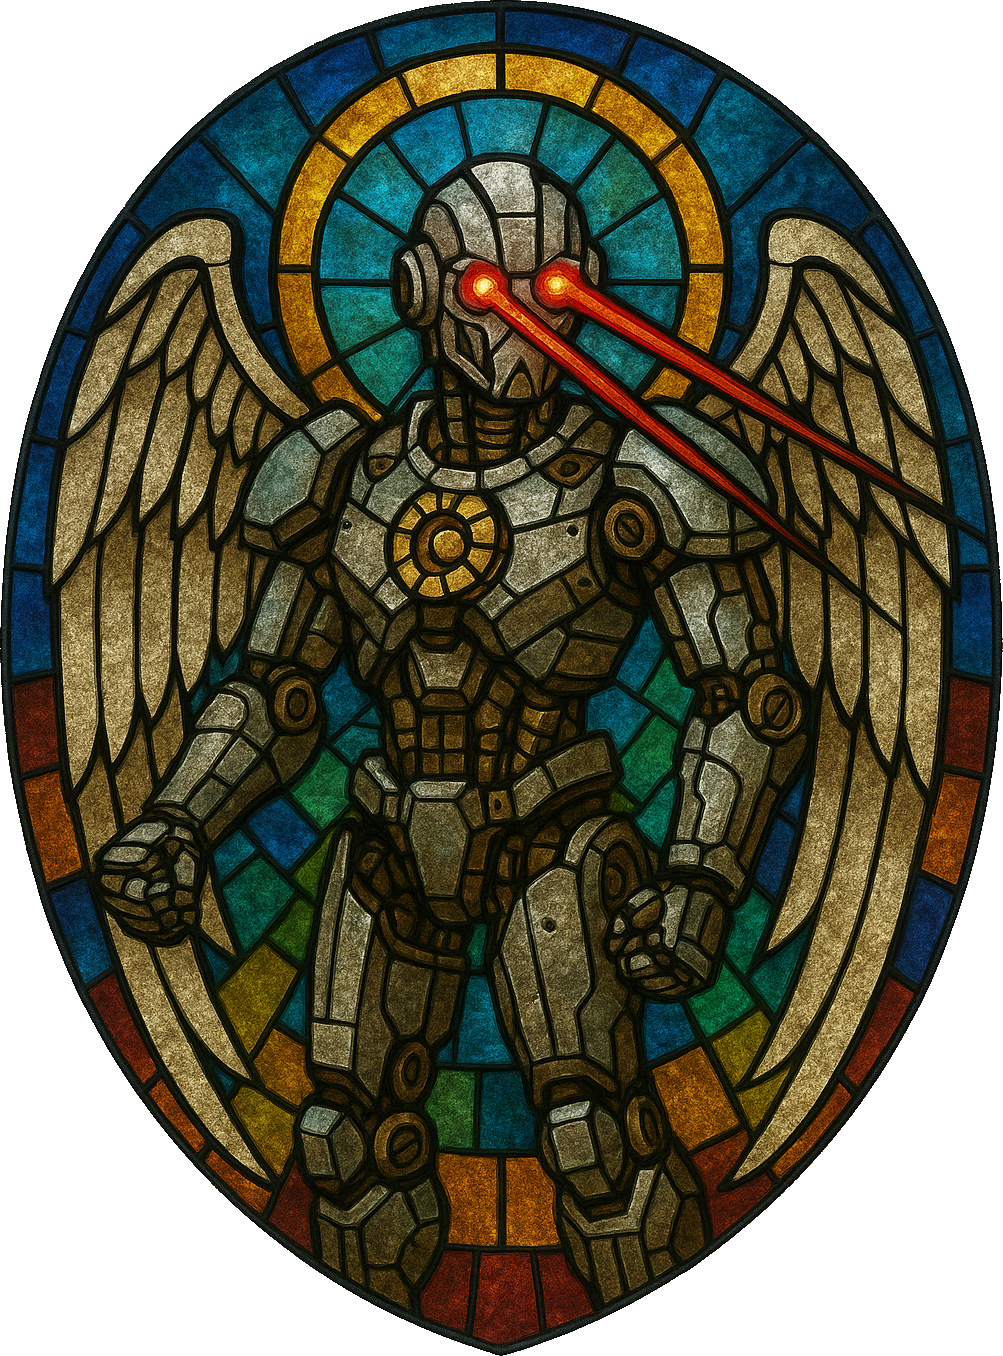
\includegraphics[width=0.1325\textwidth]{Factions/Lordship_of_Auchtertool.png}
	\end{tabular}
\end{tabular}
\vspace*{-1.65\fontdimen6\font}\hfill\\{\entryfont sentinels, and inventions that blur flesh and steel. At its head stands the Mecha-Lord - once a master artificer now encased in enchanted iron - and his heir, the Robot Prince, a sentient bronze construct powered by elemental cores. Together they guide Auchtertool as the kingdom's unrivaled nexus of magical innovation and mechanical marvels.}
\subsection*{Kingdom of Unst}
{\entryfont An island kingdom at Caledonia's northern extreme, Unst is forged in ice and storm, where brutal winters and relentless martial trials - scaling frozen cliffs, sparring on snowbound plains, hurling javelins through blizzards - shape only the toughest into warriors. Under the legendary Hootsman - said to have gargantuous beasts with bare hands - these axe-wielders ride shaggy war-beasts and wear horned helms as they honour feats of raw strength above all else. Feared for their ferocity, they reward those who prove their mettle with unbreakable loyalty.}
\subsection*{Wizards}
\subsubsection*{Courtwizards of Dundee}
\vspace*{-0.7\fontdimen6\font}\hfill\\\begin{tabular}{p{0.3\textwidth}p{0.1325\textwidth}}
	\hspace*{-1.2em}\begin{tabular}[t]{p{0.325\textwidth}}
		{\entryfont Tucked into a cramped turret overlooking the River Tay, the Courtwizards of Dundee bear a grand title belying their modest resources. Under the steady hand of a sole Master Arcanist - rumoured to be\linebreak}
	\end{tabular}
	&
	\vspace*{-2.2em}\begin{tabular}[t]{p{0.1325\textwidth}}
		
\includegraphics[width=0.1325\textwidth]{Factions/Courtwizards_of_Dundee.png}
	\end{tabular}
\end{tabular}
\vspace*{-1.65\fontdimen6\font}\hfill\\{\entryfont as wise as he is eccentric - a half-dozen apprentices toil over battered grimoires and dented athames. Their workshop is a jumble of cracked crystal balls, tarnished brass astrolabes, and wands salvaged from old duels, yet they manage to weave reliable warding spells around the ducal palace and entertain visiting nobles with small marvels of elemental fire and dancing motes of light. Ambitious but underfunded, they dream of expanding their circle - if only they could persuade the city council to replace cobwebs with coin.}
\subsubsection*{Cairngorm Mountain Wizards}
\vspace*{-0.7\fontdimen6\font}\hfill\\\begin{tabular}{p{0.3\textwidth}p{0.1325\textwidth}}
	\hspace*{-1.2em}\begin{tabular}[t]{p{0.325\textwidth}}
		{\entryfont High amid the snow-shrouded peaks of the Cairngorms lies a near-legendary conclave of wizards whose hidden village seems carved from living granite. Here, beneath ever-churning mists, the wizards practice\linebreak}
	\end{tabular}
	&
	\vspace*{-2.2em}\begin{tabular}[t]{p{0.1325\textwidth}}
		
\includegraphics[width=0.1325\textwidth]{Factions/Cairngorm_Mountain_Wizards.png}
	\end{tabular}
\end{tabular}
\vspace*{-1.65\fontdimen6\font}\hfill\\{\entryfont ancient arts of divination: obsidian runes etched with the world's fate, dream-weaving rituals performed in moonlit amphitheaters, and scrying pools said to reflect tomorrow's sun. Few pilgrims ever breach the winding passes, and of those who do, still fewer return unshaken - bearing cryptic counsel in voices heavy with portent. To meet these mountain mages is to glimpse destiny's edge... if one can decipher their whispered riddles before the wind bears them away.}
	\chapter*{Campaign Pitch}\phantomsection\addcontentsline{toc}{chapter}{Campaign Pitch}
\DndDropCapLine{B}{\entryfont rave adventurers, welcome to the land of medieval Caledonia - nowadays Scotland! This is a world of mighty warriors, arcane magic, and legendary beasts, where the echoes of battle songs ring through ancient castles and the wind carries whispers of forgotten prophecies. Here, heroes are forged in the heat of battle, kings rule by sword and spell, and unseen forces stir beneath the surface of reality.}
\subsection*{Setting}
{\entryfont The year is 992 AD.

The Kingdom of Fife stands at the dawn of a new era. Prince Angus McFife, heir to the throne, is set to wed Lady Iona McDougall, daughter of the grandmaster of Crail - an alliance that promises to bring unity and strength to both realms. As nobles, warriors, and emissaries gather in the royal city of Dundee, festivities are in full swing. The great halls are filled with music, the forges burn bright, and the people of Fife celebrate a future of peace.

Yet, across the land, whispers of unease grow louder. Strange lights flicker in the deep woods. Hunters vanish without a trace, their weapons found shattered upon the ground. In the distant mountains, the cries of beasts long thought extinct echo through the valleys. Some dismiss it as mere superstition, while others fear that something stirs in the shadows - a force unseen, waiting for the right moment to strike.

For now, the focus remains on the grand wedding, a historic moment that could shape the fate of Fife for generations to come. But in a land of heroes and legends, fate has a way of calling even the most unlikely adventurers into the fire of destiny.}
\subsection*{What to Expect}
{\entryfont\begin{itemize}
	\renewcommand\labelitemi{\textbf{\textbullet}}
	\item \textbf{Diplomatic Relations}\\Navigate the shifting politics between the Kingdom of Fife, the Knights of Crail, and other powerful factions.
	\item \textbf{Travelling across the Kingdom}\\Explore the grand halls of Dundee, the towering citadel of Crail, and the mystical Land of Unicorns.
	\item \textbf{Dungeon Delving}\\Ancient ruins, forgotten tombs, and perilous crypts hide secrets lost to time.
	\item \textbf{Skill Challenges}\\Face puzzles, riddles, and contests of skill, from solving arcane mysteries to competing in grand tournaments.
	\item \textbf{High Fantasy, High Chaos}\\Expect epic battles, legendary weapons beyond mortal comprehension, and magical beasts like unicorns, dragons, as well as large goblin hordes.
	\item \textbf{Fife, but not as you know it}\\A world of dwarven ale-forges, barbarian clans, and technological advancements. But strange disappearances and eerie omens suggest that something is not quite right in the lands of Fife.
\end{itemize}}
\vfill\eject
\subsection*{Factions}
{\entryfont\paragraph*{Kingdom of Fife} The mighty realm of King Dundax \RoyalRoman{XIII} and Prince Angus McFife, lying in eastern Caledonia. Its capital, Dundee, was founded nearly a thousand years ago by the legendary hero Dundax, who shaped the foundation of this proud kingdom. Fife is a land of noble warriors, grand castles, and rich traditions, standing as a beacon of order and strength in a realm where magic and chaos often collide.}
\hfill\vspace*{-1.7\fontdimen6\font}\\
{\entryfont\paragraph*{Templar Knights of Crail} A storied brotherhood of warriors, founded by Prolon \RoyalRoman{I} in 450 AD. Renowned for their skill in battle and their legendary eagle-riding cavalry, the Knights once waged a brutal war against the principalities of Angus and Fyfdonia in 743 AD. After years of bloodshed, the war ended in unification, forging the modern Kingdom of Fife. The Knights remain an independent and powerful force, sworn to uphold honour and justice.}
\hfill\vspace*{-0.5\fontdimen6\font}\\
{\entryfont\paragraph*{Dwarves of Caledonia: Aberdeenshi \& Methven}\hfill\\Two great dwarven clans shape Caledonia, divided by their views on magic.

The Aberdeenshi Dwarves, dwelling beneath Aberdeen and Dundee, are legendary blacksmiths, binding magic to steel to forge unmatched weapons and armor.

The Methven Dwarves, living in the Mines of Methven in the western mountains of Fife, are alchemists and brewers, crafting powerful potions and their famed enchanted ale, rumored to grant visions of the future.

Though kin by blood, the two clans clash - steel versus alchemy, forge versus flask.}
\hfill\vspace*{-0.5\fontdimen6\font}\\
{\entryfont\paragraph*{Kingdom of Unst} A fierce barbarian kingdom on an island in the far north of Caledonia, Unst is a land of harsh winters, brutal martial training, and warriors forged in the fires of endless battle. Led by the legendary Hootsman, the warriors of Unst are as wild as the storms that rage across their shores. To them, strength is everything, and only the mighty deserve to rule. Many fear their warriors, but those who earn their respect find allies of unwavering loyalty.}
\hfill\vspace*{-0.5\fontdimen6\font}\\
{\entryfont\paragraph*{Lordship of Auchtertool} A realm where magic and technology intertwine, ruled by the enigmatic Mecha-Lord and his heir, the Robot Prince of Auchtertool. The lordship stands as a hub for artificers, forge clerics, and arcane engineers, where ancient spells fuel mechanical marvels. From towering war machines to enchanted automatons, Auchtertool is a land where the boundaries of science and sorcery blur, giving birth to creations both wondrous and terrifying.}
\hfill\vspace*{-0.5\fontdimen6\font}\\
{\entryfont\paragraph*{Elves of Dùn Èideann} South past the mist shrouded Firth of Forth lies the land of the elves. In the great city's ivory spires the Aeloria weave their enchantments in once mundane objects, while deep below the Umbrasil carve crystals and grow fungi. In the living groves across the region the Sylvani sculpture their spiral homes around ancient oaks and the Mistwalkers retrive treasures and riches from the often treacherous firth.}
	
	\actpart{A Royal Wedding in Dundee}% Name of Act
	{}% Background Picture
	{0cm}% X-Shift
	{0cm}% Y-Shift
	{height=\paperheight}% Graphics-Options (height, width)
	{Act01}% Short-Handle
	{test}% URL
	{test}%	Image-Name
	{test}%	Artist

\DndDropCapLine{T}{\entryfont he campaign begins in the city of Dundee, a bustling metropolis in the heart of the Kingdom of Fife. The city is in the throes of grand celebration for the wedding of Prince Angus McFife and Lady Iona McDougall. Read aloud or paraphrase:}

\begin{DndReadAloud}
	As your party crests the final hill, the sprawling city of Dundee comes into view, its towering stone walls adorned with banners of blue and gold. The air buzzes with the sounds of celebration - cheering crowds, the lively strains of music, and the toll of bells from the grand citadel in the heart of the city.
	
	The streets are alive with bustling merchants, performers, and revellers from across the kingdom, all eager to witness the union that promises to bring peace and prosperity to the land.
\end{DndReadAloud}

\section*{The Braided Unicorn}\phantomsection\addcontentsline{toc}{section}{The Braided Unicorn}
{\entryfont Nestled in the heart of Dundee, The Braided Unicorn is a sturdy stone-built inn with a weathered slate roof and timber beams, exuding a timeless charm. Above the heavy oak door hangs a beautifully carved wooden sign of a proud unicorn, its mane braided with intricate patterns, as though prepared for some ancient, regal ceremony.

Inside, the air is filled with the scent of roasted meat, strong ale, and a hint of peat smoke. A massive hearth dominates the room, its fire crackling merrily. Above the fireplace hangs an ancient great axe, rumored to have belonged to the current owner's great-grandfather.

The tavern is run by Borin Stouthammer, a stout, no-nonsense mountain dwarf with a braided iron-grey beard and a voice like rolling thunder. He keeps a keen eye on patrons from behind the polished oak bar, where rows of wooden tankards and whisky casks line the walls. Borin is quick to laugh but quicker to enforce his rules.

At the entrance, a small board proudly displays "The Braided Unicorn's House Rules":
\begin{itemize}
	\item "Nae brawling near the bar"
	\item "If ye break it, ye buy it"
	\item "Sing in tune - or buy a round for the house"
\end{itemize}

Up a creaky staircase, cozy guest rooms await with clean beds, thick quilts, and sturdy locks on the doors - perfect for a night's rest during the city's celebrations.}
{\entryfont \paragraph*{Rumours} As the party mingles, a successful DC 12 Perception (hearing) check reveals the low murmur of an intense, anxious conversation coming from a nearby table.

The source is a group of five villagers, mostly hunters and woodsfolk, huddled close and speaking in hurried, hushed tones. Their expressions range from bewilderment to dread, and the table has several empty mugs.
\begin{itemize}
	\item \textit{"I tell ye, they weren't natural unicorns - one of 'em just stared at me, eyes black as pitch."}
	\item \textit{"Aye, and those bodies... distorted they were, like something twisted the poor beasts before killing them."}
	\item \textit{"Tis nae normal wounds! Mauled, but not like any predator I've ever seen."}
	\item \textit{"It's a plague, I say. A rabid curse! Something's got into the beasts and it's spreadin'."}
\end{itemize}
The group initially looks wary but opens up if the party approaches with care (DC 15 Persuasion check, or simply buying them a round of drinks).
\begin{itemize}
	\item They describe unicorn sightings in the nearby Dundee woods, where normally noble and peaceful unicorns have been seen acting strangely - charging madly, baring teeth, and collapsing mid-gallop.
	\item Several distorted corpses of animals (and one local hunter) have been found either mauled to death or show terrifying piercing wounds.
	\item Some whisper of a "rabid curse" or a spreading sickness. Others suggest something terrifying is lurking in the woods, frightening even the unicorns.
\end{itemize}}

{\entryfont \paragraph*{Gambling Station} At the far side of the common room, a corner is dedicated to a large, well-worn oak table surrounded by mismatched chairs. Above it hangs a cracked wooden sign with the words \textbf{"Fortune's Folly"} scrawled in faded paint. The table is always surrounded by locals, travelers, and a rotating cast of suspiciously smug regulars.

Borin Stouthammer has no patience for cheaters but allows gambling as long as it doesn't disrupt the tavern. The games played here are deceptively simple, promising quick coin - a fool's trap, as the locals say.

Players can engage with Arlen, a half elf with nimble fingers and a sharper tongue, and Breeza, a halfling dressed in flashy silks, to try their fortune in varying games:

\subparagraph*{Dice Game}
A player makes contested Deception and Insight Checks against Breeza (Breeza's Deception vs. Player's Insight and Breeza's Insight vs. Player's Deception).  The winner of each round gets 2 points to their score. If Breeza and the player tie both rolls or both win one roll each, each player gets 1 point. The first player reaching 10 points in total wins the game.

\noindent\textbf{Breeza's Cheating.} Breeza (Deception +7, Insight +5) can use Arlen as a spy gaining a +5 to her Insight rolls. Players can realize that they are cheated with a successful DC 15 (-2 for each time Breeza used Arlen to cheat) Insight Check.

\subparagraph*{The Everyman's Fireball}
Tiny, wooden objects (HP 10, AC 9, immobile) are placed on the far side of the table. Each player takes a mouthful of alcohol and spits through a flame\linebreak
\vspace*{-2.5\fontdimen6\font}\hfill\\\begin{tabular}{p{0.2\textwidth}p{0.2325\textwidth}}
	\hspace*{-0.5em}\begin{tabular}[t]{p{0.2\textwidth}}
		\vspace*{0.3em}\begin{DndTable}[header=Alcoholic Drinks]{lc}
			\textbf{Drink}	& \textbf{Strength}	\\
			Weak Beer		& 1					\\
			Regular Beer	& 2					\\
			Wine			& 4					\\
			Strong Wine		& 6					\\
		\end{DndTable}
	\end{tabular}
	&
	\vspace*{0.8em}\begin{tabular}[t]{p{0.2325\textwidth}}
		{\noindent\entryfont placed between the player and the object. Before "attacking" the object, a player must make a DC 12 Dexterity roll to not burn themselves, taking \DndDice{1d4 - 1} fire damage on a failed save. The player\linebreak}
	\end{tabular}
\end{tabular}
\vspace*{-1.6\fontdimen6\font}\hfill\\then makes a ranged attack (DEX, -4 to hit; additional -2 to hit if player failed DEX save) against the wooden object, dealing \DndDice{1d6} fire damage, but not more than the drink's strength, on a hit. After each round the objects AC and the Dexterity DC increases due to the effect the drinks have on the contestants:
\begin{itemize}
	\item Objects AC: + (Drink Strength / 3) rounded down
	\item Dexterity DC: + (Drink Strength / 2) rounded down
\end{itemize}
The first to destroy the wooden object wins the game - the game is considered a tie if both are destroyed at the same time.

\noindent\textbf{Arlen's Cheating.} If Arlen (DEX +5) hits the object or nearly misses it (AC - 3), Breeza activates a contraption that will lit up the idol dealing an additional \DndDice{1d4} fire damage to the object. A DC 17 (- amount of additional damage dealt) Insight Check reveals this cheating mechanism.
}

\subsection*{An Ape-napping}
{\entryfont As the party makes their way to exit the Braided Unicorn tavern, the door bursts open with a loud \textbf{CRASH}, nearly unhinging from its frame - The party member nearest to the door must succeed on a DC 15 Dexterity Saving Throw or takes 1 bludgeoning damage from the swung open door and is knocked prone.}

\begin{DndReadAloud}
	The door slams open with a thunderous \textbf{BANG}, silencing the tavern as a figure of regal authority strides in. A grand knight, his armour polished to a mirror-like gleam and adorned with the coat of arms of Crail, surveys the room. His breath is laboured, but his presence is unshaken, exuding an aura of command.

	\textit{"WHERE are my men?!"} he mutters, more to himself than anyone else, his voice tinged with frustration and urgency.

	His eyes settle on you, narrowing for a moment as if weighing your worth. Then, stepping forward with purpose, his voice booms with authority, yet carries a regal, almost poetic cadence:

	\textit{"You there! Adventurers! I see the fire of duty in your eyes. Will you rise to the occasion, as proud sons and daughters of Dundee? A task most urgent calls, and your valour will be met with rewards worthy of your bravery. What say thee?"}
\end{DndReadAloud}

{\noindent\entryfont Should the party express their willingness to assist, the Grandmaster will give them the details of their noble task to recover the prized ape, Bobo.}

\begin{DndQuestHook}[width=0.5\textwidth - 4pt]{Rescue Bobo}
	\DndQuestHookBasics[
		location = {The Braided Unicorn Tavern, Dundee},
		quest-giver = {Ser Proletius, Grandmaster of the Knights of Crail},
		objective = {Retrieve Prince Angus McFife's stolen pet ape, Bobo, from a bandit camp in the north-eastern woods near Dundee.},
	]
	
	{\noindent\entryfont If the party succeeds on a Survival (DC 13) check, they find signs of the camp - broken branches, footprints, and scattered food - leading them toward their destination. If they fail, they instead encounter a \hyperref[monster:BanditScout]{\LinkFont{Bandit Scout}} accompanied by two \hyperref[monster:Mastiff]{\LinkFont{Mastiffs}}. The scout attempts to fight or flee, sending one mastiff back to the camp to warn the bandits. If the scout is killed, the party can find a map to the camp on his body.

		As the party approaches the camp, they find it surrounded by several traps. A Falling Net Trap is hidden among the foliage and if triggered, the net restrains the target, and a \hyperref[monster:Bandit]{\LinkFont{Bandit}} and a \hyperref[monster:Mastiff]{\LinkFont{Mastiff}} emerge to attack. The mastiff may be sent back to warn the camp if it survives. The camp is also rigged with Warning Bell Traps. If triggered, the loud sound alerts the entire camp.

		Inside the bandit camp, the party finds two \hyperref[monster:Bandit]{\LinkFont{Bandits}} and two \hyperref[monster:Mastiff]{\LinkFont{Mastiffs}} near a wooden cage containing Bobo, the stolen pet ape. If the camp is alerted - whether by a bandit's mastiff or a warning bell - additional reinforcements arrive after two rounds: a \hyperref[monster:BanditScout]{\LinkFont{Bandit Scout}}, a \hyperref[monster:Bandit]{\LinkFont{Bandit}} and another \hyperref[monster:Mastiff]{\LinkFont{Mastiff}} - if not killed before.

		The party has options for non-lethal approaches. They can attempt to infiltrate the camp, bribe the bandits, or use stealth to avoid combat. Alternatively, the party can attempt to free Bobo quietly or with force, though loud actions will attract attention.

		Bobo, frightened but alive, is in a sturdy cage (Sleight of Hand DC 15 to lockpick with thieves' tools), and the party can calm him with food or gentle handling (Animal Handling DC 13) to ensure a smooth rescue.
	}
	
	\DndQuestRewards{Upon successfully retrieving Bobo, the party receives the following rewards from King Dundax \RoyalRoman{XIII} and Prince Angus McFife:}
	{%
		{Heroic Inspiration}{}%
		{Coupon for the Wedding Festival}{%
			Each character is given a coupon, redeemable at the festival grounds for one of the following:
			\begin{itemize}
				\item A free round of the Tree Game or Dragon's Gold games
				\item A hearty free meal at one of the many stalls
			\end{itemize}
		}%
		{Private Lodging}{As a further token of gratitude, the party is given private lodging at The Braided Unicorn, rather than having to sleep in the communal quarters. This gesture signifies their growing status in Dundee and ensures them a more comfortable stay during the wedding festivities.}
		{Tournament Entry Voucher}{This voucher allows participation in the prestigious Wedding Tourney}%
		{LEVEL-UP}{At the end of the session}
	}%
\end{DndQuestHook}
	
{\entryfont\noindent When the adventurers deliver Bobo to the commanders' tent, King Dundax \RoyalRoman{XIII}, Prince Angus McFife, and Ser Proletius express their joy and gratitude. After awarding the promised rewards, Ser Proletius will single out a barbarian, fighter, ranger, or rogue (if available) in the group by giving them the Tournament Entry Voucher and set them up for a personal challenge.}

\begin{DndReadAloud}
	Ser Proletius lips curl into a confident grin. \textit{"I challenge you to enter the Wedding Tournament. Should you reach the Jousting final, regardless of the outcome, I shall reward you with a magic item from my personal possession. But should you fail..."} He pauses, letting the moment hang in the air. \textit{"You shall join me during the wedding ceremony to sing the anthem of Crail, a song of honour, glory, and tradition."}
\end{DndReadAloud}

{\entryfont\noindent If the player successfully reached the final of the Jousting Tournament they can choose between the \textbf{Cast-Off Armour} (the armour-type can be chosen by the player) or the \textbf{Shield of Expression}.

If they win the final, Ser Proletius also allows the players to fly over the city of Dundee with the mighty Eagles of Crail.}

\begingroup
	\DndSetThemeColor[PhbLightGreen]
	\begin{DndComment}{Cast-Off Armour}
		\textit{Armour (light, medium, or heavy), common}\\
		You can doff this armour as an action.
	\end{DndComment}
	\begin{DndComment}{Shield of Expression}
		\textit{Armour (shield), common}\\
		The front of this shield is shaped in the likeness of a face. While bearing the shield, you can use a bonus action to alter the face's expression.
	\end{DndComment}
\endgroup

\chapter*{Wedding Fair}\stepcounter{chapter}\phantomsection\addcontentsline{toc}{chapter}{Wedding Fair}
\DndDropCapLine{B}{\entryfont ustling with life, Dundee's wedding fairgrounds overflow with color and sound, drawing crowds into a joyous celebration that spills into nearby streets. Bright banners ripple in the breeze, lanterns glow warmly, and the tantalizing scents of roasted meats, honeyed shortbread, and mulled cider drift through the air. At the center stands a grand oak tree, its branches adorned with ribbons and lights, casting shade over the lively gathering. Roaming the grounds is the festival's famed dragon, a marvel of craftsmanship with snapping jaws, fluttering wings, and bursts of theatrical fire that delight festival-goers. Stalls brim with Highland treats, fine tartans, and handmade goods, while performers and musicians keep the festivities alive with juggling, dancing, and lively tunes.}

\begin{DndReadAloud}
	You find yourself immersed in the sights and sounds of the wedding fair. Music from fiddles and bagpipes fills the air, weaving with laughter and the chatter of excited festival-goers. Children race between stalls, clutching candied apples and pointing in delight at jugglers tossing flaming pins. The tantalizing aroma of roasted meats and sweet shortbread tempts you at every turn.

	Nearby, a massive oak tree draped in ribbons and lanterns serves as the heart of the fair. The crowd's attention shifts as the festival's dragon - a towering, lifelike marvel of wood and metal - stirs. Its wings ripple and its jaws snap with dramatic flair eliciting gasps and cheers from the crowd.

	As the sun dips below the horizon, lanterns and torches bathe the fairgrounds in a golden glow. Laughter and awe ripple through the throng as the magic of the festival fully takes hold, drawing you deeper into its spellbinding atmosphere.
\end{DndReadAloud}

\section*{Dragon's Gold}\phantomsection\addcontentsline{toc}{section}{Dragon's Gold}
\textbf{Entry Fee:} 1 GP\\
{\entryfont The Dragon's Gold is the crown jewel of the festival, a dazzling and immersive event that draws crowds of eager participants and onlookers to the central plaza. The centrepiece of this spectacle is the magnificent dragon itself, a towering construct of painted paper, wood, and metal. Adorned with shimmering scales in vibrant reds, greens, and golds, the dragon moves with startling realism. Clever mechanisms allow its angular head to snap and jerk, its wooden wings to flutter with a show of might, and its mouth to "breathe fire" in the form of colourful ribbons and occasional bursts of magical smoke. The creature prowls menacingly near its sprawling treasure hoard, exuding an air of majesty and danger that captivates the entire square.}

\subsection*{Mechanics}
{\entryfont The Dragon's Gold game takes place in a 50-foot radius playing area, covered in thick layers of hay to conceal scattered treasures. At the heart of the area lies the 15-foot radius Inner Hoard, where the most coveted prizes are clustered. However, this inner zone is guarded by the festival dragon, which relentlessly defends its treasures.}

\begin{DndMonster}[width=0.5\textwidth]{Festival Dragon}
	\DndMonsterType{Large Construct, neutral good}
	
	% If you want to use commas in the key values, enclose the values in braces.
	\DndMonsterBasics[
		armor-class = {16},
		hit-points  = {\DndDice{9d10 + 36}},
		speed       = {20 ft.},
	]
	
	\renewcommand{\AbilityScoreSpacer}{~}
	\DndMonsterAbilityScores[
		str = 7,
		dex = 7,
		con = 18,
		int = 8,
		wis = 18,
		cha = 20,
	]
	
	\DndMonsterDetails[
		saving-throws = {CON +8, CHA +9},
		skills = {Insight +8, Intimidation +9, Perception +8},
		%damage-vulnerabilities = {cold},
		%damage-resistances = {bludgeoning, piercing, and slashing from nonmagical attacks},
		%damage-immunities = {poison},
		senses = {Passive Perception 18},
		%condition-immunities = {poisoned},
		languages = {-},
		challenge = -,
		proficiency-bonus = +4,
	]
	
	\DndMonsterSection{Traits}
    \DndMonsterAction{Operative Mastery}
    The Festival Dragon must be operated by a group of at least 6 people. If the Festival Dragon is operated by a properly trained performing team, its AC is increased by 2 and gains a bonus of +4 to each melee attack and damage roll.
    
	\DndMonsterAction{Non-Lethal Attacks}
	Each attack the Festival Dragon makes is considered non-lethal
	
	\DndMonsterAction{Friendly Nature}
    The Festival Dragon is usually friendly towards children and only chases them away, unless they get too greedy.
	
	\DndMonsterSection{Actions}
	\DndMonsterAction{Multiattack}
	The Festival Dragon makes one Claw Attack and one Bite or Tail Attack.
	
	\DndMonsterAttack[
		name=Claw,
		distance=melee, % valid options are in the set {both,melee,ranged},
		%type=weapon, %valid options are in the set {weapon,spell}
		mod=-2,
		reach=5,
		%range=20/60,
		targets=one target,
		dmg=\DndDice{1d4 - 2},
		dmg-type=slashing,
		%plus-dmg=\DndDice{1d6},
		%plus-dmg-type=poison,
		%or-dmg=,
		%or-dmg-when=,
		extra={ (minimum of 1 damage)},
	]
	
	\DndMonsterAttack[
		name=Bite,
		distance=melee, % valid options are in the set {both,melee,ranged},
		%type=weapon, %valid options are in the set {weapon,spell}
		mod=-2,
		reach=5,
		%range=20/60,
		targets=one target,
		dmg=\DndDice{1d6 - 2},
		dmg-type=piercing,
		%plus-dmg=\DndDice{1d6},
		%plus-dmg-type=poison,
		%or-dmg=,
		%or-dmg-when=,
		extra={ (minimum of 1 damage)},
	]
	
	\DndMonsterAttack[
		name=Tail,
		distance=melee, % valid options are in the set {both,melee,ranged},
		%type=weapon, %valid options are in the set {weapon,spell}
		mod=-2,
		reach=20,
		%range=20/60,
		targets=one target,
		dmg=\DndDice{1d6 - 2},
		dmg-type=bludgeoning,
		%plus-dmg=\DndDice{1d6},
		%plus-dmg-type=poison,
		%or-dmg=,
		%or-dmg-when=,
		extra={ (minimum of 1 damage)},
	]
	
	\DndMonsterAction{Breath Weapon (Recharge 5 Rounds)}
	Each creature in a 30ft. long, 5 ft. wide line must make a DC16 Dexterity Saving Throw or are instantly out of the Dragon's Gold game.
	
	\DndMonsterSection{Reactions}
	\DndMonsterAction{Automated Construct}
	The Festival Dragon can make one attack of opportunity with each of its front limbs, mouth, and tail.
\end{DndMonster}

{\entryfont\noindent Participants enter the game unarmed and unarmoured, with no equipment allowed. The use of magic is strictly prohibited, and contestants may not harm or attack one another under any circumstances, preserving the festive nature of the game.

Each round lasts 2 minutes (20 rounds in total). Contestants have this time to search for and claim as much treasure as they can manage.

To locate treasures, contestants may perform one of the following actions:
\begin{itemize}
	\renewcommand\labelitemi{\textbf{\textbullet}}
	\item \textbf{Spot Check (Perception):} Roll against a DC20 Check to locate a treasure anywhere in the play area (DC15 if searching within the Inner Hoard).
	\item \textbf{Search Check (Perception):} Roll against a DC10 Check to locate a treasure in a specific 5-foot square. Searching in this way within the dragon's reach provokes an Attack of Opportunity from the dragon.
\end{itemize}
If a contestant succeeds on either check, they can roll on the Treasure Table to determine the item found.

Contestants may continue to search and gather treasure for as long as they wish, carrying as many items as they can manage. However, treasures are forfeited if a contestant is struck by the dragon's attack and "killed". To remain in the spirit of the game, "dead" contestants are expected to leave the game when they are struck and may not interact with the hoard further, though they can remain in place as casualties for the remainder of the game.}

{\entryfont\noindent Contestants may leave the treasure hoard at any time, taking their gathered loot with them. Once a contestant leaves the playing area, they cannot re-enter. Leaving the area ends their participation in the game.\\\\
The balance of greed and caution defines the game: contestants must weigh the temptation of more treasures against the risk of provoking the dragon's wrath. The most daring and resourceful participants will walk away with riches, but those who overreach may lose everything!}

\begin{DndTable}[header=Treasure Table]{lXX}
\textbf{d100}	& \textbf{Outer Hoard (value)}							& \textbf{Inner Hoard (value)}	\\
01-10			& A small mound of 3d6 cp								& A mound of 5d6 sp				\\
11-20			& A shell bracelet (2 sp)								& Costume jewellery (1 gp)		\\
21-30			& A bag filled with coloured stones and marbles (5sp)	& A finely article of clothing, tied with ribbon (5 gp) \\
31-40			& A wreath of flowers and ribbons (2 sp)				& A large box that holds many rich candies (2gp) \\
41-50			& An embroidered cloth with a picture (1 gp)			& Bronze jewellery set with semi-precious stones (5gp) \\
51-60			& A wooden token good for a free meal at a local restaurant (5sp)	& A dagger or short-sword in sheath (10 gp) \\
61-70			& A toy sword painted silver (2 sp)						& A metal flask filled with spirits (2 gp) \\
71-80			& A gold coin (1 gp)									& A pretty doll or toy (5 gp) \\
81-90			& Some type of art supply, like inks, pens, fancy wood, or paint (3 gp)	& A common item made of silver or gold, like a needle (10 gp) \\
91-100			& Roll on the Inner Hoard table at +10					& Fancy jewellery or clothing (50 gp)
\end{DndTable}

\begin{DndOptionalRule}{Attack the Dragon}
	The Festival Dragon can be attacked during the Dragon's Gold Game with weapons and weapon-like items that are found during the game. However, it is not allowed to use any kind of magic to damage the construct.
\end{DndOptionalRule}

\section*{Tree Game}\phantomsection\addcontentsline{toc}{section}{Tree Game}
\textbf{Entry Fee:} 1 GP\\
{\entryfont The Tree Game is a lively and challenging test of accuracy and skill, where contestants attempt to claim prizes nestled among the high branches of a towering tree. Using arrows, handaxes, or throwing knives, competitors aim for trinkets, baubles, and even valuable treasures carefully lodged within the tree's limbs. Each well-placed strike sends a prize tumbling gracefully to the ground, greeted by the crowd's cheers - or the envious gazes of onlookers hoping for their turn.}

\begin{DndReadAloud}
	Before you stands a majestic oak, its sprawling branches adorned with glittering prizes that catch the light like stars in the daylight. Trinkets dangle from ribbons and strings, while more valuable treasures are wedged tightly into crooks and knots high above. The lower branches sway gently with small, easy-to-reach prizes, while the loftiest rewards glint enticingly just out of easy range. Contestants gather at the base of the tree, readying their arrows, handaxes, or knives as the crowd murmurs in anticipation.

	\textit{"Step forward and take your shot!"} calls the event's master of ceremonies. \textit{"What will you claim from the tree's bounty - luck, skill, or sheer determination?"}

	The air hums with excitement as the first competitor lines up their throw, aiming to send fortune falling from the great tree's branches.
\end{DndReadAloud}

\subsection*{Mechanics}
{\entryfont In the Tree Game, contestants are tasked with dislodging prizes tied to the branches of the grand festival tree using borrowed weapons provided by the game organizers. Each participant may choose either a shortbow with 5 arrows or two handaxes, both of which must be returned at the end of the game. Over the course of five rounds, contestants attempt to target and knock down the dangling prizes, each taking a single shot or throw per round.

Using the shortbow requires precise aim, as contestants must hit the harder AC (standard-AC +2) listed in the Prize Table to sever the ribbons holding the prizes in place. Conversely, handaxes rely on brute force, allowing contestants to attack against the standard AC of the target. Regardless of the weapon used, any prize that is successfully dislodged and falls to the ground is immediately claimed by the contestant.}

\begin{DndTable}[header=Prize Table]{llX}
\textbf{Height}	& \textbf{Effective AC}			& \textbf{Prize}												\\
10-24 ft		& 11 (13)						& Dart, Bucket, Piton, Signal Whistle							\\
25-39 ft		& 13 (15)						& Ladder, Sling Bullets (40), Sling								\\
40-44 ft		& 15 (17)						& Javelin, Lamp, Blanket, Sealing wax							\\
45-49 ft		& 18 (20)						& Arrows (20), Crossbow Bolts (20), Hammer, Caltrops (bag of 20)\\
50 ft +			& 18 (20)						& Padded Armour, Handaxe, Pike, Healer's kit					\\
\end{DndTable}

\begin{DndOptionalRule}{Losing Thrown Item}
	Critical Failure (NAT 1) leads to the thrown item to be stuck in the tree as well, and needs to be retrieved/dislodged in a similar manner like the prizes. Otherwise it will be lost to the game.
	
	For each borrowed hand axe lost during the game the contestant has to pay 10GP (40GP for a lost shortbow).
\end{DndOptionalRule}
\chapter*{Wedding Tourney}\stepcounter{chapter}\phantomsection\addcontentsline{toc}{chapter}{Wedding Tourney}
\DndDropCapLine{T}{\entryfont he Wedding Tourney celebrating the union of Angus McFife I and Iona McDougall has brought an air of excitement and festivity to Dundee. The grand event unfolds with a series of thrilling competitions, drawing skilled participants and eager spectators from across the land. The day's revelry begins with an archery contest and progresses through feats of strength and skill, including the long throw and the challenging log chop. Competitors earn points in each event based on their finishing positions, with their accumulated scores determining the seeding for the climactic jousting competition. In this final contest of valour and chivalry, the ultimate winner of the tourney will be crowned, marking the joyous celebration's triumphant conclusion. The point-scoring\linebreak}

\vspace*{-4.6\fontdimen6\font}\hfill\\\begin{multicols}{2}
{\entryfont \noindent system for the Wedding Tourney is designed to reward consistent performance across the Archery, Long Throw, and Log Chopping competitions. Competitors earn points based on their\linebreak}
\vspace*{-2.2em}\begin{DndTable}[header=Point Scoring System]{lXr}
\textbf{Rank}	&& \textbf{Points}	\\
1st				&& 10				\\
2nd				&& 8				\\
3rd				&& 6				\\
4th				&& 4				\\
5th				&& 2				\\
6th				&& 1				\\
\end{DndTable}\\
\end{multicols}
\vspace*{-4.3\fontdimen6\font}\hfill\\

{\noindent\entryfont finishing positions in each event, with the highest total scores determining their seeding for the jousting competition.}

\section*{Bullseye's Glory}\phantomsection\addcontentsline{toc}{section}{Bullseye's Glory}
{\entryfont The archery competition marks the opening event of the Wedding Tourney, testing the precision and steady hands of each competitor. Standing 80 feet away from a stationary target, each archer must demonstrate their mastery over the shortbow, aiming true to score as many points as possible. Crowds gather to watch as the competitors take their shots one by one, the rhythmic twang of bowstrings ringing through the air as arrows fly toward the bullseye. This contest of skill requires calm focus and careful aim, setting the tone for the challenging events to follow.}

\subsection*{Mechanics}
{\entryfont In the archery competition, each contestant has four shots to score points based on their aim and accuracy. To make each shot, competitors roll an attack against the target, with their point total determined by the roll's outcome, as detailed in the provided Scoring Table. All competitors must use an unenchanted shortbow, provided by the tourney organizers, to ensure fair play; any archer found using enchanted equipment will be immediately disqualified.}
\begin{DndTable}[header=Archery Scoring]{lXX}
\textbf{Attack Roll}	& \textbf{Location}		& \textbf{Points}	\\
less than 8				& Miss					& 0					\\
8+						& Outer Ring			& 1					\\
11+						& Middle Ring			& 3					\\
14+						& Inner Ring			& 5					\\
17+						& Bullseye				& 10				\\
NAT20					& Split another Arrow	& 10 + \textit{Crowd Roar*}	\\
\end{DndTable}
{\footnotesize * \textit{Crowd Roar} gives a +2 to the next attack roll in this competition.}
\vfill\eject
\begin{tikzpicture}[remember picture, overlay]%
	\node[xshift=0.25cm, yshift=0.25cm, anchor=north east] at (current page.north east) {\includegraphics[width=.6\paperwidth]{%
		images/Landscape/Archery_Competition%
	}};%
\end{tikzpicture}%
\hfill\\ \\ \\
\begin{DndTable}[header=Archery Ranking]{lXl}
\textbf{Rank}	& \textbf{Name}					& \textbf{Points}	\\
1st				& Ewan MacRae of Dunkeld		& 28				\\
2nd				& Gavin Buchanan				& 19				\\
3rd				& Rory MacTavish				& 14				\\
4th				& Alasdair MacLeod				& 8					\\
5th				& Hamish "Halfwit" McGregor		& 1					\\
\end{DndTable}

\section*{Hurl of Might}\phantomsection\addcontentsline{toc}{section}{Hurl of Might}
{\entryfont The Long Throw Competition is a test of raw power, technique, and endurance, as competitors attempt to throw a series of progressively heavier and more unwieldy objects as far as possible. Each object presents a unique challenge, requiring not only physical strength but also skillful control to reach impressive distances. Spectators gather eagerly along the marked field, cheering as each competitor heaves their object through the air, striving for the farthest distance in each throw. This contest celebrates feats of might and mastery, with each participant vying to surpass their rivals in sheer throwing range.}

\subsection*{Mechanics}
{\entryfont In the Long Throw Competition, contestants must throw four distinct objects, each with its own weight and difficulty, as outlined in the provided table. Each competitor has two attempts with each object, and only the best throw for each object counts toward their total score. Each throw requires a DC 10 check to clear the first range increment, and every additional 4 points above the DC increases the throw's range by one increment, as defined in the table. The contestant can use specific skills (also noted in the table) to attempt each throw. If the object's weight exceeds twice the contestant's Strength Score in pounds, they must roll with disadvantage due to the strain of hefting the object. The contestant's gain points for each distance increment, with the competitor achieving the greatest total declared the victor of the Long Throw Competition.}

\begin{DndTable}[header=Thrown Objects]{lllX}
\textbf{Object}	& \textbf{Range}				& \textbf{Weight}		& \textbf{Skill(s)}					\\
Javelin			& 30 ft.						& 2 lbs					& STR								\\
Discus			& 20 ft.						& 5 lbs					& Athletics (STR), Acrobatics (DEX)	\\
Stone			& 10 ft.						& 18 lbs				& STR, DEX							\\
Halfling		& 5 ft.							& 30 lbs				& STR								\\
\end{DndTable}

\begin{DndTable}[header=Long Throw Ranking]{lXl}
\textbf{Rank}	& \textbf{Name}					& \textbf{Points}	\\
1st				& Ewan MacRae of Dunkeld		& 13				\\
2nd				& Alasdair MacLeod				& 10				\\
3rd				& Rory MacTavish				& 6					\\
4th				& Gavin Buchanan				& 4					\\
5th				& Hamish "Halfwit" McGregor		& 2					\\
\end{DndTable}

\section*{Timber Trial}\phantomsection\addcontentsline{toc}{section}{Timber Trial}
{\entryfont The Log Chopping competition is a thrilling display of strength, stamina, and quick decision-making, as contestants race against the clock to chop through as many logs as they can in a single minute. With logs standing at regular intervals, participants must strike quickly and move swiftly to cover the ground between each target, chopping one after another in a relentless rhythm. Spectators cheer on as wood chips fly and axes swing, creating an intense spectacle of determination and power. The choice of weapon might play a key role, as each contestant must decide between speed and force, adjusting their approach to maximize their tally. Only the most determined and strategic log chopper will claim victory in this demanding event.}

\subsection*{Mechanics}
{\entryfont In the Log Chopping competition, contestants have one minute (10 rounds) to destroy as many logs as possible. Each log has an AC of 15 and 18 HP, challenging competitors to balance force and accuracy with each swing. The logs are spaced 10 feet apart, requiring contestants to move to the next log after each one is destroyed. At the start of the competition, contestants select a weapon from the provided weapon rack, which holds 2 \textbf{Handaxes} (1d6 slashing, light), a \textbf{Battleaxe} (1d8 (1d10 versatile) slashing), and a \textbf{Greataxe} (1d12 slashing, heavy, two-handed). They may switch weapons during the contest, but doing so requires a full round to return to the rack and select a new weapon. The contestant who destroys the most logs within the allotted time is declared the winner, with any ties broken by the lowest HP remaining on the last partially damaged log.}

\begin{DndTable}[header=Log Chopping Ranking]{lXl}
\textbf{Rank}	& \textbf{Name}					& \textbf{Points}	\\
1st				& Hamish "Halfwit" McGregor		& 10*				\\
2nd				& Ewan MacRae of Dunkeld		& 5 (18 HP)			\\
3rd				& Alasdair MacLeod				& 3 (12 HP)			\\
4th				& Rory MacTavish				& 2	(6 HP)			\\
5th				& Gavin Buchanan				& 1 (12 HP)			\\
\end{DndTable}
{\footnotesize * Hamish has used an illegal Adamantine Axe for this challenge and will be disqualified after the competition}

\section*{The Grand Joust}\phantomsection\addcontentsline{toc}{section}{The Grand Joust}
\begin{DndReadAloud}
	Before you stretches the grand jousting arena, a testament to the kingdom's dedication to noble sportsmanship and spectacle. The tiltyard is a long, sandy stretch bordered by wooden rails, with pennants in vibrant colors fluttering from high poles. Rows of wooden stands rise on either side, packed with eager onlookers waving banners of the Kingdom of Fife. At the center of the stands, the royal box gleams with ornate carvings and golden accents, where the bride and groom sit with their court, overseeing the proceedings with regal anticipation. Squires and attendants scurry along the perimeter, preparing horses and lances while the competitors mount up for the first tilt. The air is electric with the sound of cheering, the smell of trampled earth, and the thrill of impending glory.
\end{DndReadAloud}

\subsection*{Mechanics}
{\entryfont Based on their performances in the earlier contests - the Archery, Long Throw, and Log Chop - the champions have been seeded: the first-ranked competitor will face the fourth, and the second will challenge the third. Only the victors of these matches will move on to the final joust to determine the champion of the tourney.}
\subsubsection*{Mount Familiarization}
{\entryfont Before engaging in the joust, each competitor must take time to familiarize themselves with their mount. This crucial moment allows them to build a bond of trust and control, ensuring their steed responds with precision during the high-stakes contest.}

{\entryfont Each participant must make a DC 15 Animal Handling Check to gauge how well they connect with their mount.
\begin{itemize}
	\renewcommand\labelitemi{\textbf{\textbullet}}
	\item \textbf{Success:} The rider gains a +1 bonus to their first Ride (Constitution) check during the joust.
	\item \textbf{Critical Success (Natural 20):} The rider gains a +2 bonus to their first Ride (Constitution) check and an additional +1 bonus to a potential subsequent Ride (Constitution) check.
	\item \textbf{Critical Failure (Natural 1):} The rider suffers a -2 penalty to their first Ride (Constitution) check and a -1 penalty to all subsequent Ride (Constitution) checks for the duration of the competition.
\end{itemize}}
\subsubsection*{The Joust}
{\entryfont After familiarizing themselves with their mounts, the contestants ride onto the tiltyard for the main event. The jousting competition is a dramatic test of precision, strength, and endurance. Riders charge toward one another, their tourney lances poised to strike, as the crowd cheers in anticipation of every thunderous impact.

Contestants use specially crafted tourney lances provided by the organizers. These lances deal 1d4 piercing (non-lethal) damage. If a rider deals more than 10 damage in a single round, the lance shatters spectacularly, earning the rider a +2 bonus to their next attack roll as the crowd cheers their impressive display of skill and power.

The use of magic during the joust is strictly forbidden and results in immediate disqualification.

Each pass between the two contestants is resolved through simultaneous strikes. Riders may choose one of the following attack strategies for their turn:

\begin{itemize}
	\renewcommand\labelitemi{\textbf{\textbullet}}
	\item \textbf{Aim at Helmet:}
	\begin{itemize}
		\item Attack Roll Penalty: -8 to attack roll.
		\item If the attack lands, the opposing rider must make a Ride (Constitution) Check with a DC of 15 + damage dealt to stay mounted.
	\end{itemize}
	\item \textbf{Crouch defensively:}
	\begin{itemize}
		\item Attack Roll Penalty: -4 to attack roll.
		\item The rider gains a +4 bonus to their Ride (Constitution) Check if struck.
	\end{itemize}
\end{itemize}

\noindent When struck by an opponent's lance, a rider must make a Ride (Constitution) Check (DC 5 + damage dealt) to remain in the saddle. Any rider reduced to 0 HP will automatically fail this check.

\noindent The unseated rider must succeed on a DC 15 Athletics or Acrobatics Check to land safely. On a failed check, the rider takes 1d6 bludgeoning damage from the fall.

If both riders remain mounted after a pass, the joust continues into another round. The DC for all subsequent Ride (Constitution) Checks increases by +2 after each round to represent the mounting tension and fatigue of the contest. The joust ends when only one rider remains mounted. That rider is declared the winner.

If both riders are unseated in the same round, the contest escalates into a melee duel to determine the victor. Both contestants are armed with blunt shortswords (1d4 bludgeoning, non-lethal) provided by the organizers. The duel continues as a standard one-on-one melee fight, with both riders retaining the hit points and damage accumulated during the joust. The first contestant to submit or fall unconscious loses the joust.}

\subsection*{"Party-cipation"}
{\entryfont The jousting finale may be centred on one member of the party, but the bonds of friendship and camaraderie run deep. This optional rule allows the rest of the party to actively contribute to their champion's performance, giving them a chance to support and influence the outcome in meaningful ways. Whether through cheering, strategizing, or even small magical gestures (within the festival's rules, of course), the party's involvement can turn the tide in a close contest. Following are some ideas that can be implemented:
\begin{itemize}
	\renewcommand\labelitemi{\textbf{\textbullet}}
	\item \textbf{Hype up the Crowd}\\
	The party members can use their turn to cheer, chant, or otherwise encourage their champion. Doing so requires a successful Charisma (Performance) Check DC 13 to hype up the crowd and giving the following benefits:
	\begin{itemize}
		\renewcommand\labelitemii{\textbf{\textbullet}}
		\item \textbf{Success}\\
		The champion gets a +2 bonus on either the next attack roll or the next Ride (Constitution) Check.
		\item \textbf{Critical Success}\\
		The champion also gains temporary hit points equal to the party members' highest Charisma modifier (minimum of 1).
		\item \textbf{Critical Failure}\\
		The next attack roll and a possible Ride (Constitution) Check are made with disadvantage.
	\end{itemize}
\end{itemize}
\vfill\eject
\begin{itemize}
	\renewcommand\labelitemi{\textbf{\textbullet}}
	\item \textbf{Crowd Manipulation}\\
	A particularly charismatic party may attempt to rally the crowd to their champion's favour. This requires a Charisma (Persuasion) or Charisma (Deception) Check (DC 20).
	\begin{itemize}
		\renewcommand\labelitemii{\textbf{\textbullet}}
		\item \textbf{Success}\\
		The crowd becomes fully invested in the champion's success, granting a +2 bonus to their attack rolls for the next two rounds.
		\item \textbf{Critical Success}\\
		The crowd's overwhelming support inspires the champion, giving them advantage on all checks and attack rolls for the next two rounds.
		\item \textbf{Failure}\\
		The crowd's disapproval leads to the champion being distracted, having disadvantage on the next attack and potential Ride (Constitution) check.
		\item \textbf{Critical Failure}\\
		The crowd immensely disapproves of the champion, giving them disadvantage on all checks and attack rolls for the next two rounds.
	\end{itemize}
\end{itemize}
}
\subsubsection*{Boon of the Crowd}
{\entryfont If the party influenced the match (through cheering or crowd manipulation), the champion gains the following boon:
\begin{itemize}
	\item The champion can re-roll a failed Ride (Constitution) Check or attack roll during the joust.
\end{itemize}
}

\section*{Tourney Prizes}\phantomsection\addcontentsline{toc}{section}{Tourney Prizes}
{\entryfont \paragraph*{Winner} The Winner of this prestigious tourney will be known throughout the Kingdom of Fife which will have some benefits but also drawbacks later in this campaign if a player is able to win the tournament. A player also gets a \textbf{Heroic Inspiration} and 200 GP.}
{\entryfont \paragraph*{2nd Place} The 2nd placed contestant gets 100 GP.}
{\entryfont \paragraph*{3rd / 4th Place} The 3rd and 4th placed contestants get 25 GP each.}

\begin{tikzpicture}[remember picture, overlay]%
	\node[yshift=-0.6cm, anchor=south] at (current page.south) {\includegraphics[width=\paperwidth]{%
		images/Landscape/Jousting_Tourney%
	}};%
\end{tikzpicture}%
\chapter*{Wizard Tower of Dundee}\stepcounter{chapter}\phantomsection\addcontentsline{toc}{chapter}{Wizard Tower of Dundee}
\noindent \textit{Feel free to treat this puzzle-filled Wizard Tower as an optional side-quest. It exists simply to give your group a light, puzzle-focused break before the \hyperref[chapter:UnicornInvasionOfDundee]{\LinkFont{Unicorn Invasion of Dundee}} truly unfolds. Since the invasion deserves its own dedicated session (and shouldn't be broken up), this adventure lets you occupy a play session with clever challenges and exploration before diving headlong into the spectacular battle to come.}\\
\DndDropCapLine{U}{\entryfont pon arriving at the Wizard Tower of Dundee, the party encounters a magnificent wooden door set into the stone façade. Its surface is covered in intricate, fading runes and arcane depictions - stars, planetary symbols, and scenes of spellcasting - yet years of neglect have left it streaked with rusted metal fittings and patches of moss clinging to its edges.}

\begin{DndReadAloud}
	As you step onto the cobblestones of Dundee's wizard quarter, the Tower of Dundee looms above you - a spiraling gray stone keep etched with glowing runes. Set into the base of its wall is a grand wooden door, once opulent, now aged and weathered. Intricate arcane symbols and depictions of spellcasters cover its panels, but rusted iron straps streak across the wood, and patches of moss curl around its edges, as if nature itself seeks to reclaim it.

	Before you can examine it further, a young woman in immaculate azure robes approaches, her robes embroidered with the tower's crest. Her lips curve into a polite but condescending smile as she crosses her arms.

	\textit{"And what, may I ask"}, she says in a crisp, clipped tone, \textit{"draws you to the Tower of Dundee? Curiosity, ambition, or something else entirely?"}
\end{DndReadAloud}

{\noindent\entryfont No matter how the door is opened - lockpicking, kicking it in, or casting Knock - the moment the door yields by any means (or the word "Time" is spoken nearby), a hidden ward activates. Instantly, every member of the party and the snooty student Eilidh MacKenzie are thrown into separate puzzle chambers within the tower.}

\section*{Puzzle Rooms}\phantomsection\addcontentsline{toc}{section}{Puzzle Rooms}
{\entryfont This segment presents a sample framework for the puzzle chambers that lie beyond the warded door. Feel free to design entirely new challenges tailored to your group - this example is merely illustrative. In it, each player is whisked into a distinct room shaped by their character's (sub-)class, while a central chamber remains pitch black. Eilidh MacKenzie, who always lands in the darkened hub, knows the Light Cantrip and will harshly scold any spellcaster there who can't cast it.}

\subsection*{Central Chamber}
\textbf{{\entryfont Correct Combination:} 947}\\
{\entryfont The central chamber is magically linked to all outer rooms, allowing occupants of those rooms to communicate with the central hub, but the outer rooms cannot do so directly with one another.}

\begin{DndReadAloud}
	As the ward's magic ripples through you, darkness swallows your senses. You feel the chill of damp stone beneath your feet and hear distant, echoing drops of water. Soon after, a single point of light ignites near your shoulder - Eilidh glares at you from across the void, her fingertips aflame with a soft, bluish glow.
	
	Around you, three round stone pillars loom out of the black: each carved with ten faintly recessed glyphs depicting the digits 0 through 9 in a clockwise ring. In front of the middle stele stands a tall, conical funnel of weathered stone, crowned by a gigantic, multifaceted crystal that seems to pulse with arcane energy. A simple wooden table nearby holds a lone sheet of parchment.
\end{DndReadAloud}

{\noindent\entryfont Within this chamber, the party must piece together a three-digit code by interpreting the riddle on the \hyperref[resource:WizardTowerPuzzleRiddle]{\LinkFont{Parchment}} and find clues in each outer room. Once they believe they have the correct combination, any member - or Eilidh (+5 to hit) - can attempt a ranged spell attack against the crystal (DC 5). Depending on whether the combination is accurate, one of the following will occur:
\begin{itemize}
	\item \textbf{Success:} The crystal flares, teleporting everyone (including Eilidh) into Professor Ambric's Arcanum.
	\item \textbf{Failure:} An arcane alarm sounds and Modrons appear according to the Modron Encounter Table.
\end{itemize}
}
\begin{DndTable}[header=Modron Encounter Table]{llX}
	Failure	& Monsters														& Room	\\
	1st		& 1 \hyperref[monster:ModronMonodrone]{\LinkFont{Monodrone}}	& Central Chamber	\\
	2nd		& 2 \hyperref[monster:ModronMonodrone]{\LinkFont{Monodrone}}	& Each Room			\\
	3rd		& 2 \hyperref[monster:ModronDuodrone]{\LinkFont{Duodrone}}		& 2 Random Rooms	\\
	4th		& 2 \hyperref[monster:ModronTridrone]{\LinkFont{Tridrone}}		& Other 2 Rooms		\\
	5th+	& 1 \hyperref[monster:ModronQuadrone]{\LinkFont{Quadrone}}		& Each Room			\\
\end{DndTable}

\subsection*{Clockwork's Puzzle}
{\entryfont The Clockwork Chamber displays a marvel of different ancient but also futuristic mechanical apparitions. At the center of the room stand two identical pedestals - each forged from burnished brass and dark-stained oak - supporting five concentric rings that can spin independently. At first glance, every ring is covered in fractured lines and scattered letters that form no recognizable pattern.}
\begin{DndReadAloud}
	You find yourself in a low, metal-clad chamber, the air humming with faint mechanical whirs. In the center, two brass-and-oak pedestals stand side by side, each bearing five concentric rings stacked like an elaborate wheel. The rings are covered in jagged, half-formed lines and scattered letters that make no sense at first glance. Tiny polished handles protrude from each ring, inviting you to manipulate them.

	Faint inscriptions circle the base of each stand, worn but still readable under the flickering and blinking lights projected by several mechanical apparitions. Above the rings, you notice a pair of tiny glass lenses - perhaps meant to magnify something, should the rings fall into place correctly.
\end{DndReadAloud}
{\noindent\entryfont Each device is engineered so that, when its rings are aligned just right, a secret image and iconography "snap" into view. On the first pedestal, the rings collapse into a stylized unicorn head, whereas, on the second pedestal, the completed rings form a stout warhammer. As soon as each symbol set locks, the scrambled letters on its rings shift into crisp typography, spelling out "ARROW" on the first device and "SWORD" on the second device.}
\begingroup
	\DndSetThemeColor[DmgSlateGray]
	\begin{DndComment}{Real-World Implementation}
		\textit{Cut five concentric paper rings and fasten them at the center - do this twice. On one set, draw a unicorn head, on the other, a warhammer. Scatter letters on each ring so that, when aligned correctly, the unicorn device spells "ARROW" and the warhammer device spells "SWORD". Turning the paper layers replicates the puzzle's rotating mechanism.}
	\end{DndComment}
\endgroup

\subsection*{Hunter's Puzzle}
{\entryfont The Hunter's Chamber evokes the misty Highland forests of Scotland, dominated by the ruins of an ancient, weathered stone temple nestled in a moonlit clearing. The air is thick with the sharp scent of pine and damp earth, broken only by the soft rustling of leaves overhead. Above this silent tableau, two faintly glowing sigils drift among the debris: one takes the graceful shape of a unicorn, the other the sturdy form of a warhammer.}
\begin{DndReadAloud}
	You find yourself in a quiet clearing beneath towering evergreens, the scent of pine mingling with damp earth. Before you stands a weathered stone temple at the clearing's edge - its columns leaning and draped in moss. At your feet lie shattered arrows, battered swords, and bleached bones, as though relics of hunts long past.

	Faintly glowing symbols catch your attention: one shaped like a unicorn, the other a stout warhammer. As you fix your gaze on the symbols arrows, bones, and swords seem to react and start glowing and shifting. The scattered items seem to be pointing you toward a hidden pattern - one that promises to reveal the sequence you seek.
\end{DndReadAloud}
{\noindent\entryfont To succeed here, the party must remember that the unicorn symbol corresponds to "ARROW" and the warhammer symbol corresponds to "SWORD" from the previous chamber. When they focus on the unicorn glyph, nearby arrows should shift; when they focus on the warhammer glyph, swords should move.}
\begingroup
	\DndSetThemeColor[DmgSlateGray]
	\begin{DndComment}{Real-World Implementation}
		\textit{To build this physically, start by printing or sketching a weathered temple scene on sturdy paper. On a separate sheet of semi-transparent vellum, draw the glowing unicorn and warhammer symbols - and a hidden unknown symbol - in corresponding positions. Place the vellum over the temple image and align the symbols exactly. Next, on the base image (beneath the vellum), draw arrows, swords, and bone fragments so that when you match each symbol on the overlay, tracing lines over the aligned items forms the digits of your puzzle combination. In play, handing the vellum to the player allows them to hold it over the temple picture, trace the items highlighted by each symbol, and reveal the hidden numbers.}
	\end{DndComment}
\endgroup

\subsection*{Smith's Puzzle}
{\entryfont This chamber exists to confirm the correct sequence of the three digits uncovered in the other rooms. By now, the party should possess the numbers "4", "7", and "9".}
\begin{DndReadAloud}
	Flickering torchlight glints off coals in multiple forges, each hearth roaring with heat. The scent of molten metal and coal hangs heavy in the air. Anvils stand ready atop stout legs, bellows rest against stone walls, and workbenches overflow with hammers, tongs, and metal scraps.

	Directly opposite the main entrance, you notice a large wooden rack adorned with ten weapons - axes, swords, maces, polearms, and more. Above each piece is a digit from 0 to 9, carved into the polished wood.
\end{DndReadAloud}
\noindent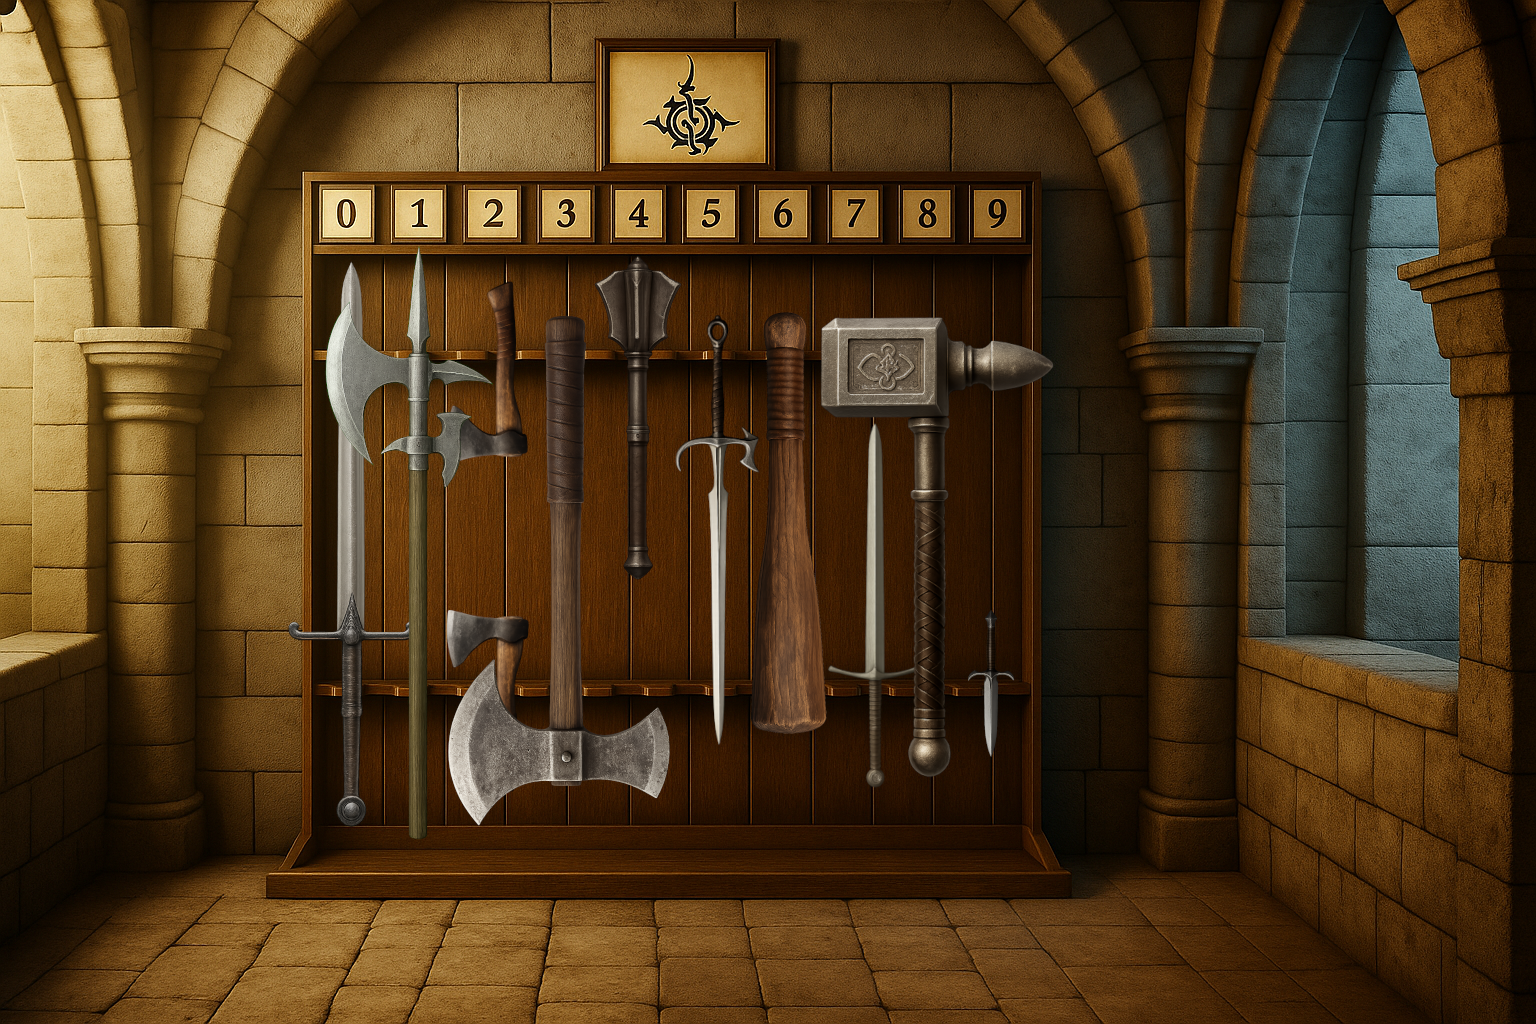
\includegraphics[width=\linewidth]{Puzzles/Weapon_Rack}

{\noindent\entryfont On this weapon rack, each number corresponds to a specific weapon: 4 is the mace, 9 is the dagger, and 7 is the longsword. To determine the proper order, players must arrange these three weapons by their damage dice - in ascending order from lowest to highest.}

\section*{Headmaster's Arcanum}\phantomsection\addcontentsline{toc}{section}{Headmaster's Arcanum}
{\entryfont The Arcanum is an impeccably maintained study, its polished marble floor reflecting the soft glow of arcane sconces. Every shelf and cupboard is completely void of books and artifacts, as though each volume was removed with deliberate care mere hours ago. There are no scuff marks or signs of disorder - only faint impressions on the dustless surfaces where tomes once rested. Drawers are closed flush, and the velvet rug lies perfectly centred before the fireplace. The sole remaining object is a leather-bound volume titled \textbf{"On the History of Master Arcanists"}, placed deliberately in the center of the mahogany desk. The lingering scent of fresh ink and parchment suggests Professor Ambric organized the space recently, then departed.}
\begingroup
	\DndSetThemeColor[PhbLightGreen]
	\begin{DndComment}{On the History of Master Arcanists}
		\textit{A book containing the history and description of the following spells:
		\begin{itemize}
			\item Jim's Magic Missile
			\item Melf's Acid Arrow
			\item Melf's Minute Meteor
			\item Leomund's Secret Chest
		\end{itemize}
		These spells can be copied into a spellbook.}
	\end{DndComment}
\endgroup
\chapter*{Wedding Ceremony}\stepcounter{chapter}\phantomsection\addcontentsline{toc}{chapter}{Wedding Ceremony}
\DndDropCapLine{W}{\entryfont ith the Grand Joust concluded and the dust of the arena settled, the realm turns its eyes toward the Wedding Ceremony. Nobles and warriors, emissaries and jesters, all gather beneath the soaring banners of the Kingdom of Fife, bearing witness to the sacred union that will shape the future of the land.}

{\entryfont The air is filled with the soft melodies of minstrels, the quiet murmur of conversation, and the distant toll of ceremonial bells. The feast is prepared, the finest ales poured, and every detail has been arranged to honour this momentous occasion. As the ceremony begins, the weight of history settles upon those in attendance - this is more than a union of two souls; it is a bond that will shape the future of the realm.}

\subsection*{Lost Bet}
{\entryfont Should a player have lost their bet with Ser Proletius their fate is now inescapable. The grandmaster, ever the showman, seizes the moment, throwing a jubilant arm around the unlucky soul and pulling them toward the center of the stage.}
\begin{DndReadAloud}
	\textit{"A debt is a debt, my friend!"} Proletius declares, his voice booming over the gathered guests. \textit{"And tonight, we shall hear your voice in all its glory!"}

	With a grand gesture, he signals the minstrels, who immediately begin playing the first triumphant notes of \textbf{The Anthem of Crail}. The crowd erupts in cheers, awaiting your performance - whether you sing with the heart of a true Knight of Crail, fumble awkwardly through forgotten lyrics, or attempt some last-ditch trickery to escape your fate.
\end{DndReadAloud}

\section*{Dwarven Keg of Chaos}\phantomsection\addcontentsline{toc}{section}{Dwarven Keg of Chaos}
{\entryfont A relic of mirth and mystery, the Dwarven Keg of Arcane Chaos is a legendary wedding tradition among the dwarves of the Mines of Methven, nestled deep within the western mountains of the Kingdom of Fife. Said to have been crafted by the Brewlords of Old, the keg is not bound by mortal hands - instead, it is infused with the raw, unpredictable essence of arcane fermentation.

The Methven dwarves believe that drinking from the keg is a blessing of fortune and folly alike - a way for fate to weave its hand into the revelry of a grand occasion. No two drinks are ever the same, and those who partake may find themselves endowed with temporary gifts, burdened by absurd curses, or simply confused as to why they now possess a perfectly baked meat pie.

It is tradition among the dwarves that the keg be brought forth at grand unions and feasts of great joy, for a wedding without chaos is a wedding doomed to boredom. Legends claim the first Grandmaster of Crail himself drank from its frothy depths and spent an entire evening levitating uncontrollably while composing a ballad about cheese wheels - a song still sung in dwarven halls to this day.}
\begin{tikzpicture}[remember picture, overlay]%
	\node[xshift=0.25cm, yshift=-0.25cm, anchor=south east] at (current page.south east) {\includegraphics[width=.5\paperwidth]{%
		images/Props/Pocket_Meat_Pie%
	}};%
\end{tikzpicture}%
\begin{DndTable}[header=Magical Effects]{cX}
	1d10	& Effect \\
	1 		& \textbf{Beard of Glory}\newline You grow a magnificent beard, regardless of gender. For the next hour you have advantage on Charisma (Persuasion) rolls.\\
	2		& \textbf{Tongue of the Brewlord}\newline For the next 5 minutes you can only speak, read and understand Dwarven. (Primordial if you already can speak and understand Dwarven)\\
	3		& \textbf{The Floor is Lava!}\newline You think that the whole floor is lava. You have to jump from object to object to move through the room. If you touch the floor in any way, you take \DndDice{1d4} Psychic damage. This effect persists for 1 minute or until you take damage.\\
	4		& \textbf{Mithral Stomach}\newline For 1 hour you are immune to poison - even alcoholic poisoning - and can eat anything.\\
	5		& \textbf{Jolly Jig}\newline A random dwarven drinking song fills your mind. You must make a DC 12 Wisdom Saving Throw or dance and sing for the next minute.\\
	6		& \textbf{Echoing Belch}\newline Your next burp is so loud that it can be heard 300 feet away. Small or tiny creatures that can hear the burp must succeed on a DC 15 Wisdom Saving Throw or are frightened for 1 minute.\\
	7		& \textbf{Dwarven Gourmet}\newline For the next 10 minutes you have developed an absolute love for the dwarven cuisine. You may demand for ale-soaked mushrooms, stone-bread, or lava-boiled snails for the duration of this effect.\\
	8		& \textbf{Mysterious Pocket Snack}\newline You find a still warm meat pie (\DndDice{2d4 + 2} Temporary Hit Points when eaten) in your pocket. How did it get there? It smells delicious.\\
	9		& \textbf{Bard's Curse}\newline For the next 5 minutes whenever you try to speak, you instead sing your words in a dramatic ballad-like fashion.\\
	10		& \textbf{Blessing of the Brewlords}\newline A faint golden glow surrounds you. For the next hour you have advantage on Charisma Checks when dealing with dwarves. Also, dwarves will offer you free drinks.
\end{DndTable}

\vfill\eject

\section*{Seer's Confection}\phantomsection\addcontentsline{toc}{section}{Seer's Confection}
{\entryfont At the heart of the wedding feast, standing upon a pedestal of ornate silver and enchanted stone, rests a cake of mysterious origin and whispered legend. Though no one can say exactly where it came from, it is known to appear only at the most significant unions in history - always present, yet never explained. Some believe it to be the work of the Cairngorm Wizards, the enigmatic spellcasters of the western reaches, while others insist it is a creation of fate itself, woven from threads of time and possibility.

The nobility refer to it in hushed tones as \textit{"The Seer's Confection"}, a name that carries both awe and caution. The legends claim that those who partake will experience visions of their destiny, glimpsing possible futures - some glorious, some tragic, some utterly incomprehensible. However, fate does not reveal itself lightly, and the cake's magic is not without risk.}
\begin{DndTable}{cX}
	1d100	& Vision/Effect \\
	1 		& You fall into a \textit{Destiny Coma}. When the player is woken up he speaks the words of \textbf{"Anstruther's Dark Prophecy"}, but cannot recollect the words or the reason why afterwards.\\
	2-20	& \textit{Destiny Coma}\\
	21-40	& \textit{You glimpse the rippling surface of a vast, mist-covered lake, just as something massive and serpentine slips beneath the water - too distant to see clearly, yet leaving behind an unnatural stillness that lingers long after the vision fades.}\\
	41-60	& \textit{In the far corner of the Braided Unicorn Tavern, half-hidden beneath a worn, dust-covered rug, you glimpse the outline of a trapdoor - its edges marked by age and secrecy. A faint draft of cold, earthy air whispers from its seams, hinting at a tunnel descending into darkness.}\\
	61-80	& \textit{You see a woven basket resting tipped over on the earth - its lid lying next to it - near the edge of what appears to be the early foundations of the city of Dundee, silent and bathed in golden morning light.}\\
	81-99	& You have a vision of three items: a Battlehammer, an Amulet, and a Dagger.\\
	100		& You speak the words of \textbf{"Anstruther's Dark Prophecy"}.
\end{DndTable}
\subsection*{The Destiny Coma}
{\entryfont For some, the sheer magnitude of the destinies they witness is too much to bear. Their minds become lost in the flood of possibility, their bodies collapsing into unconsciousness as they struggle to grasp what they have seen. This state, known as the Destiny Coma, has struck down kings, knights, and scholars alike. While most awaken quickly with aid, some never return at all, their minds forever lost in the depths of fate's tapestry.

Should one succumb to the Destiny Coma, they experience the following effect:}
\begingroup
	\DndSetThemeColor[PhbMauve]
	\begin{DndComment}{Destiny Coma}
		\textit{You are overwhelmed by the many destinies you see and fall unconscious, taking \DndDice{1d6} Psychic damage. You can only be woken up by a healing spell/potion - a Goodberry is sufficient - or you are hit after 1 minute of being unconscious, taking at least 1 bludgeoning damage.}
	\end{DndComment}
\endgroup

\vfill\eject

\section*{Floating Goblets}\phantomsection\addcontentsline{toc}{section}{Floating Goblets}
\begin{tikzpicture}[remember picture, overlay]%
	\node[xshift=0.25cm, yshift=0.25cm, anchor=north east] at (current page.north east) {\includegraphics[width=.25\paperwidth]{%
		images/Props/Hobgoblet_Shuffleboard%
	}};%
\end{tikzpicture}%
{\entryfont Tucked into a shadowed corner of the bustling\\grand plaza, a small table draws a lively crowd.\\ Laughter, cheers, and playful jeers rise above\\the din, as people gather around what appears\\to be a simple game - yet there's a spark of\\excitement, and perhaps mischief, in the air.

The "stall" is hosted by the charismatic\\Lady Belissa and the quick-tongued Sir Alrik the Swift, both commanding the crowd with practised flair and contagious energy. However, beneath their convincing appearances, these two are in fact the notorious Breeza and Arlen in masterful disguise.

Only a successful DC 30 Wisdom (Insight) Check reveals subtle clues - a familiar piece of jewelry worn by "Belissa", or a fleeting speech quirk in "Alrik's" banter - hinting at their true identities beneath the disguises. To everyone else, they remain just another pair of colourful revellers adding their own brand of excitement to the festivities.}

\subsection*{The Hobgoblet Shuffleboard}
{\entryfont A Player Character and Alrik (Sleight of Hand +2) each take turns sliding a goblet down the polished table (Dexterity Sleight of Hand Check), aiming for marked scoring zones at the far end. The goal is to accumulate the highest total score over three rounds.}

\begin{DndTable}[header=Shuffleboard Scoring]{lXX}
\textbf{Roll}	& \textbf{Location}		& \textbf{Points}		\\
less than 8		& Too Short				& 0						\\
8+				& First Zone			& 1						\\
12+				& Second Zone			& 2						\\
16+				& Third Zone			& 3						\\
NAT20			& Right on the Edge		& 3	- chance to cheat	\\
20+				& Too Long				& 0						\\
\end{DndTable}

{\entryfont \paragraph*{Cheating} The hosts still cannot move away from their cheating ways and again created a sophisticated cheating mechanism to turn the odds in their favour. The table can be tilted by Belissa to ensure a goblet either moving further - even off the table - or stopping earlier than expected.

Whenever Sir Alrik takes his turn, Lady Belissa subtly tilts the table at just the right moment, allowing her to adjust Alrik’s roll by up to $\pm 4$. Additionally, if an opponent rolls a natural 20, Belissa can discreetly interfere - shifting the balance of the table just enough to cause the goblet to veer off and fall, nullifying what would have been a perfect shot.

The player or a bystander can notice this kind of cheating with a successful DC 15 Wisdom (Perception) Check and possibly intervene.}\\\\
{\entryfont \paragraph*{Fleeing Revellers} If the players catch Belissa and Alrik cheating, they slip into the crowd and vanish, leaving behind a small pouch of valuables:
\begin{itemize}
	\item 75GP
	\item Cantrip Scroll of Minor Illusion
\end{itemize}
}

\vfill\clearpage

\section*{Encounters}\phantomsection\addcontentsline{toc}{section}{Encounters}
{\entryfont As the ceremony turns to celebration, the wedding feast offers a rare chance to speak with key figures of great importance. Conversations held tonight may reveal hidden truths, forge alliances, or stir tensions yet unseen.}

\subsection*{Prince Angus McFife}
{\entryfont On this day, Prince Angus McFife is the happiest man in the world. His love for Iona McDougall is evident in every word he speaks, every glance he steals in her direction. He radiates joy, pride, and an unwavering belief in the future, knowing that their union will bring peace and prosperity to the kingdom.

Angus is genuinely pleased to see so many people from all corners of Fife gathered for the festivities. Unlike many nobles, he is deeply interested in the lives of others, eagerly asking the party about their backgrounds, their adventures, and what brought them to this moment.}
\subsubsection*{Stance on the Highland Mysteries}
{\entryfont Angus does not dismiss the danger, knowing that people - real people - have died or gone missing, even if the stories themselves are exaggerated or wrapped in legend. What frustrates him most is his father's reluctance to act, as King Dundax \RoyalRoman{XIII} sees the tales as nothing more than superstitious nonsense.

Angus knows arguing with his father is futile, but that does not mean he does nothing. If he cannot fight the cause directly, he will fight for and support the families left behind.}
\subsection*{King Dundax \RoyalRoman{XIII}}
{\entryfont The esteemed ruler of the Kingdom of Fife, King Dundax \RoyalRoman{XIII}, welcomes conversation with a regal yet measured presence. He speaks at length about the history of the kingdom, its alliances, and the broader landscape of power across the land. His focus remains on matters of diplomacy, legacy, and the future of Fife, offering insights into the realm's political state and its standing among neighbouring territories.}
\subsubsection*{Stance on the Highland Mysteries}
{\entryfont When the topic of strange sightings in the Highlands arises he reacts with mild amusement and scepticism. Dismissing them as superstitious nonsense, he considers such tales to be nothing more than the fancies of fearful peasants or exaggerations from overzealous hunters. He expresses no real concern, seeing no reason to divert attention from more pressing political matters.}
\subsection*{Ewan MacRae of Dunkeld}
{\entryfont If a party member faced Ewan MacRae in the Grand Joust, the stalwart protector of Dunkeld greets them with genuine admiration, praising their skill and courage in battle. He remarks that it's rare to meet someone who can truly hold their own, offering an invitation to share a drink in good company.

Ewan proves to be a welcoming and honourable man, eager to speak of his beloved city of Dunkeld and the responsibility he bears in protecting its people. He takes great pride in his duty, ensuring that the city remains safe from both external threats and the dangers of the wilds beyond its borders.}
\subsubsection*{Stance on the Highland Mysteries}
{\entryfont When asked about the mysteries of the Highlands, Ewan's expression darkens for a moment as he falls into deep thought. In a quieter voice, he admits that the hunters of Dunkeld have spoken to him about strange occurrences in the mountains and forests that lie beyond the kingdom's heartlands. Their stories are too detailed, too consistent, to be dismissed as mere folklore.

Yet, Ewan is no fool - he knows that openly speaking about such matters would invite scepticism and ridicule. Instead, he keeps his concerns private, though he remains curious and watchful, eager to uncover the truth behind whatever truly lurks in the Highlands.}
\subsection*{Princess Iona McDougall}
{\entryfont \paragraph*{Bobo was rescued} If the party successfully rescued Bobo, Iona McDougall seeks them out personally, her usual composed demeanour replaced by genuine gratitude. She expresses her deep appreciation for their actions and rewards them with a \hyperref[magicalitem:HeartPureOfSteel]{\LinkFont{Heart pure of Steel}}, ensuring they know how much their deed means.}
{\entryfont \paragraph*{Bobo is still missing}
If the party failed to rescue Bobo, her tone is far more solemn. She informs them that while Angus McFife does not outwardly show his grief, she can see the weight of his sorrow beneath the surface. The loss has affected him deeply, and though he will never speak of it, his heart is heavy.}
\subsubsection*{Stance on the Highland Mysteries}
{\entryfont Iona is concerned not for the strange sightings themselves, but for the people who have vanished - hunters, adventurers, and those who set out never to return. She worries for the families left behind, the unexplained absences, and what may be lurking in the Highlands. However, as for the stories of "rabid" unicorns and other legends, she remains largely indifferent, dismissing them as embellishments on a real and more troubling reality.}
\subsection*{Grandmaster Ser Proletius}
{\entryfont A conversation with Ser Proletius is never a quiet affair. The Grandmaster of the Knights of Crail speaks with unshakable pride about his order, boasting of their glorious deeds, unwavering honour, and unmatched skill in battle. He never misses an opportunity to praise the Knights of Crail, often weaving grand tales of past victories - sometimes exaggerated, sometimes entirely true. Despite his loud and boastful nature, he is not without humour, readily laughing at a well-placed jest and responding in kind with his own repertoire of knightly jokes and tales.}
\subsubsection*{Stance on the Highland Mysteries}
{\entryfont If there is a threat to the realm, Ser Proletius swears he would hunt it down and strike it down himself, should he ever uncover the truth. However, when it comes to the tales of "rabid" unicorns and other Highland legends, he finds himself torn between scepticism and caution. While he doesn't dismiss the rumours outright, he is equally unwilling to waste time chasing after ghost stories. If a true danger exists, he believes it will reveal itself soon enough - and when it does, he will be the one to put an end to it.}
\chapter*{Unicorn Invasion of Dundee}\stepcounter{chapter}\phantomsection\addcontentsline{toc}{chapter}{Unicorn Invasion of Dundee}\label{chapter:UnicornInvasionOfDundee}
\DndDropCapLine{F}{\entryfont lea-ridden bedding, creaking floorboards, and the lingering odour of stale ale and mildew - the deplorable conditions of within the Braided Unicorn are not suited for a good-nights rest. Any character who sleeps there automatically gains one level of exhaustion.}

{\entryfont Elves, constructs, and those who secured private lodging may attempt a DC 15 Constitution saving throw to resist the effects. If an elf or construct enjoyed the comfort of a private room, they make this saving throw with advantage.}

\begin{DndReadAloud}
	Your restless slumber is shattered by a deafening explosion that rocks the tavern. The ground trembles beneath you, and dust fills the air as distant screams echo through the chaos. A blinding flash outside is followed by a crack of thunder, and you see fireballs raining down from the skies.

	Through the grimy window, you glimpse a scene of pure carnage. Blackened plumes of smoke coil into the dawn sky as undead soldiers march through the flaming streets. Among them, corrupted unicorns charge through the chaos, killing and mauling the unfortunate and defenceless townsfolk.

	Another explosion shakes the tavern, and from downstairs, the frantic voice of the barkeep cries out: \textit{"They're here! The monsters are here! We're doomed!"}
\end{DndReadAloud}

\begin{DndOptionalRule}{Hasty Departure}\label{or:HastyDeparture}%
	When the party is abruptly roused by chaos in the Braided Unicorn, they may flee in haste, leaving behind non-essential adventuring gear such as rations and backpacks. They retain only their equipped items, quest essentials, gold, and perhaps a few potions.
\end{DndOptionalRule}

\section*{The Last Stand}\phantomsection\addcontentsline{toc}{section}{The Last Stand}
{\entryfont The barkeeper frantically urges the party to help barricade the tavern's two windows and the front door against the oncoming undead horde.

Each window requires two party members working together. A window will be successfully barricaded if the players succeed twice before failing twice during this skill challenge. For example, a players can make a DC 14 Strength (Athletics) or Dexterity (Sleight of Hand) check (or use appropriate tool proficiencies such as Carpenter's Tools).

If at least one window is successfully barricaded no undead will break through it on Turn 2. If both are successfully barricaded also on Turn 4 no new undead will appear.}
\subsection*{Encounter: Fight to Survive}
{\entryfont This encounter resembles a Monster Rush:
\paragraph*{Enemies} 2 \hyperref[monster:UndeadSoldier]{\LinkFont{Undead Soldiers}} appear at the start of the encounter. On initiative count 20 of each round after the first, 2 more undeads will breach through windows. At the start of the 3rd turn additionally a \hyperref[monster:CorruptedUnicorn]{\LinkFont{Unicorn}} will breach through the barricaded door and attack the barkeep. On initiative count 20 of the 5th turn the tavern is obliterated by a fireball, killing everyone within the tavern.
\paragraph*{End of Battle} The only goal is to flee through the tunnel beyond the trap door, pointed out by the barkeeper shortly before he is mauled and beheaded by the unicorn. As soon as all players reached the trap door the battle ends and the tavern is obliterated above them.}

\section*{The Fall of Dundee}\phantomsection\addcontentsline{toc}{section}{The Fall of Dundee}
{\entryfont Moments after the party enters the tunnel, a fireball crashes into the tavern above, obliterating the structure with a deafening roar. The tunnel shakes as debris collapses behind them, sealing the exit and forcing them forward towards the unknown.}

\begin{DndReadAloud}
	Emerging from the tunnel, you step into a scene of chaos and despair. The acrid stench of smoke fills your lungs, and the sky above burns with fire and crackling lightning. Flames consume the nearby buildings, casting flickering light over the main plaza of Dundee, now a battleground. Soldiers of the kingdom and a few desperate citizens fight valiantly, but they are hopelessly outnumbered by the relentless undead soldiers and grotesque, corrupted unicorns. The screams of the dying echo all around, mixing with the roars of undead beasts and the clash of steel.
	
	At the heart of the plaza, you see a familiar figure: King Dundax \RoyalRoman{XIII}, a golden figure in the darkness. His shining armor reflects the fiery glow of the battlefield as he duels several undead soldiers. With every swing of his blade, he fells another foe, standing as a beacon of courage amidst the carnage. For a fleeting moment, hope flickers in your hearts.
	
	But then it happens!

	A corrupted unicorn, its rotting flesh gleaming wetly and its glowing, jagged horn crackling with dark energy, bursts through the melee. With terrifying speed, it lowers its head and charges. The king barely has time to turn before the horn pierces through his golden breastplate, the force lifting him off the ground.

	Time seems to freeze as King Dundax \RoyalRoman{XIII}, the proud ruler of the Kingdom of Fife, collapses to the bloodstained cobblestones. His crown falls, rolling a few feet before stopping at the hooves of the monstrous beast.

	Around you, the battle continues, but it is clear: the heart of the kingdom has just been torn away. This is not just the fall of a city - it may well be the end of Fife itself.
\end{DndReadAloud}

\subsection*{Encounter: The King is Dead}
{\entryfont The corrupted unicorn and two undead soldiers that felled King Dundax \RoyalRoman{XIII} notice the party. With bloodlust in their hollow, glowing eyes, the creatures pivot from their prior target and focus on the adventurers. The undead soldiers advance in a disciplined formation, shields raised and weapons ready, while the corrupted unicorn lets out a bone-chilling, unnatural whinny, pawing the ground as it prepares to charge. The party has no choice but to fight for their survival amidst the chaos of the main plaza.

\paragraph*{Enemies} 2 \hyperref[monster:UndeadSoldier]{\LinkFont{Undead Soldiers}}, 1 \hyperref[monster:CorruptedUnicorn]{\LinkFont{Corrupted Unicorn}} (47 HP, no Teleport)

\paragraph*{Tactics} The undead soldiers will engage in combat first, aiming to tie up melee combatants while the unicorn uses its mobility to keep the party under pressure. The unicorn may charge at a spellcaster or ranged attacker after observing the battlefield.

\paragraph*{Support} If a player is hit by the Charge Attack or is hit by any attack while at 5 HP or below, \hyperref[char:SerProletius]{\LinkFont{Ser Proletius}} and \hyperref[char:AngusMcFife]{\LinkFont{Prince Angus McFife}} appear to help the party in the battle. Ser Proletius will charge in front of the attacked player and use his Divine Allegiance feature to take the hit instead. During the fight Ser Proletius heals the party members and protects them, while Prince Angus McFife fights along with them.

\paragraph*{End of Battle} If the unicorn is below 10 HP or both Undead Soldiers are dead, the battle will end and the evil wizard Zargothrax will appear (continue reading).
}
\section*{Unholy Coronation}\phantomsection\addcontentsline{toc}{section}{The Unholy Coronation}
{\entryfont The evil wizard Zargothrax, clad in robes of dark energy, makes his entrance atop a massive undead unicorn. His arrival heralds the city's fall, as fear and despair grip the defenders. The party witnesses his terrifying entrance, setting the stage for his declaration as the dark master of Dundee.}
\begin{DndReadAloud}
	A sudden chill grips the air, and the battlefield falls eerily silent for a fleeting moment, as though the city itself is holding its breath. Then, from above, a shadow spreads across Dundee, dark and foreboding.
	
	Through the smoke and fire, a figure emerges atop a towering, undead unicorn of war. The creature's skeletal form crackles with violet energy, its empty eye sockets burning with an eerie, unholy light. It moves with an unnatural grace, its very presence pressing down upon the battlefield like an unspoken command to submit. The few remaining defenders shrink back, their weapons trembling in unsteady hands.

	The unicorn's hooves land upon the bloodied stones of the plaza, sending a ripple of necrotic energy through the ground. A silence falls, not of peace, but of resignation - of finality. Then, a voice cuts through the air, cold and commanding, laced with dark amusement and absolute authority.

	\textit{"People of Dundee! Your king is dead. Your city is mine. Kneel before me, and perhaps I will grant you the mercy of undeath."}
	
	For a moment, the battlefield stands frozen, the weight of the proclamation hanging like a curse over the ruined city. Then - Ewan MacRae, bloodied but unbroken, charges through the haze of battle, sword raised high. His face is set with unshaken determination as he rushes toward the figure atop the undead steed.
	
	\textit{"FOR DUN-"}
	
	But before he can close the distance, he jerks violently mid-stride - his body convulsing as an unseen force seizes him. His sword clatters to the ground - he collapses onto the cobblestone, lifeless. No wounds mark his body. His charge ended in an instant, his final words forever unfinished.
	
	\textit{"PATHETIC MORTAL SCUM! KILL THEM ALL! FROM THIS DAY FORWARD, I, LORD ZARGOTHRAX, RULE DUNDEE!"}
	
	With these words, the sky, once pitch-black, erupts into an inferno of searing light, as if the heavens themselves burn in response to his unholy coronation.
\end{DndReadAloud}

{\noindent\entryfont The inferno in the sky is no natural phenomenon - it is a devastating barrage of fireballs, cascading down upon Dundee like the wrath of a vengeful god. The battle is over. There is no victory to be found here.}

\section*{Flee Certain Death}\phantomsection\addcontentsline{toc}{section}{Flee Certain Death}
{\entryfont As the destruction unfolds and the undead army overruns the last defences, Ser Proletius and Prince Angus McFife waste no time in shouting above the chaos - Dundee is lost. The city and townsfolk were not ready for war. To stay is to die. With no other choice, they urge the party towards the River Tay Bridge, the only remaining escape route.}

\subsection*{Navigating the Burning Ruins}
\begin{DndReadAloud}
	The streets are collapsing, buildings are crumbling, and undead soldiers prowl the alleys. You must find a safe route to the River Tay Bridge before you are trapped inside the city.
\end{DndReadAloud}
\subsubsection*{Goal}
{\entryfont Find a secure path through the fire and destruction.}
\subsubsection*{Skill Checks}
{\entryfont Each PC makes one check as it is a team effort to navigate safely through what seems like the apocalypse.}
\paragraph*{Perception (DC 12)}
{\entryfont Spot a safer, less-collapsed route through the city.}
\paragraph*{Survival (DC 12)}
{\entryfont Predict which building is closest to collapsing and avoid dangerous areas.}
\paragraph*{Acrobatics (DC 12)}
{\entryfont Leap over burning debris or collapsed rooftops to take shortcuts.}
\paragraph*{Investigation (DC 12)}
{\entryfont Identify an escape route hidden between buildings and rubble.}
\subsubsection*{Outcome}
\paragraph*{3+ Successes}
{\entryfont The party moves swiftly, avoiding unnecessary danger.}
\paragraph*{1-2 Successes}
{\entryfont The party takes some damage from falling debris (\DndDice{1d4} bludgeoning damage).}
\paragraph*{0 Successes}
{\entryfont They are caught in a collapsing street, taking \DndDice{1d4 + 2} bludgeoning damage and gaining one level of exhaustion as they free themselves from the rubble.}

\subsection*{Pass the Undead Horde}
\begin{DndReadAloud}
	As you navigate the war-torn streets of Dundee, you see a group of undead soldiers cut down fleeing townsfolk. Beyond the carnage, the River Tay Bridge stands, but to reach it, you must find a way past these relentless killers... or cut through them.
\end{DndReadAloud}
\subsubsection*{Goal}
{\entryfont Sneak past the undead horde or engage in battle, fighting your way through them and towards your escape.}
\subsubsection*{Skill Checks}
{\entryfont Each PC makes one check aiding to find a way and sneaking past the undead soldiers.}
\paragraph*{Stealth (DC 15)}
{\entryfont Weave through burning and collapsed buildings to avoid detection.}
\paragraph*{Athletics (DC 15)}
{\entryfont Smash through weakened structures to create a new escape route.}
\paragraph*{Intimidation (DC 15)}
{\entryfont Shout commands to confuse and frighten the undead.}
\paragraph*{Deception (DC 15)}
{\entryfont Trick the undead into hesitating searching for you.}
\paragraph*{Sleight of Hand (DC 15)}
{\entryfont Quickly unlock a barricaded side gate leading toward the bridge.}
\subsubsection*{Outcome}
\paragraph*{5 Successes}
{\entryfont The party finds and saves a little child hiding in the rubble (+1 Heroic Inspiration for each PC). They successfully sneak past the relentless killers.}
\paragraph*{3-4 Successes}
{\entryfont The party stealthily bypasses the enemies without combat.}
\paragraph*{0-2 Successes}
{\entryfont The undead detect the players, and the party must fight anyway (reinforcements will arrive 1 turn earlier).}
\subsubsection*{Combat}
{\entryfont If the party decides to engage in combat or are detected by the enemies they are attacked by 5 \hyperref[monster:UndeadSoldier]{\LinkFont{Undead Soldiers}} (20 HP). Angus McFife and Ser Proletius can join the battle. On Initiative Count 20 on Turn 5 reinforcements (2 \hyperref[monster:UndeadSoldier]{\LinkFont{Undead Soldiers}} and 1 \hyperref[monster:CorruptedUnicorn]{\LinkFont{Unicorn}}) will arrive - Turn 4 if the party failed to sneak past the horde.}

\subsection*{The Final Sprint over the Bridge}
\begin{DndReadAloud}
	As you near the River Tay Bridge, fireballs hammer the ancient stonework, sending tremors through the ground as chunks of masonry crumble into the raging waters below. The entire structure groans under the assault, shaking violently beneath your feet.

	From ahead, Ser Proletius and Prince Angus McFife turn back, their eyes wide with urgency.

	\textit{"MOVE NOW! RUN!"}

	A deafening crack splits the air as another fireball slams into the bridge. The supports buckle. The path behind you is collapsing.

	There is not much time to make it across...
\end{DndReadAloud}
\subsubsection*{Goal}
{\entryfont Sprint across the collapsing River Tay Bridge to reach the far side before it crumbles into the waters below. Safety is uncertain, but staying behind means certain death.}
\subsubsection*{Skill Checks}
{\entryfont This is a frantic individual challenge - each PC must rely on their own speed and reflexes to survive.
\begin{itemize}
	\renewcommand\labelitemi{\textbf{\textbullet}}
	\item \textbf{Athletics (DC 13):} For those with trained endurance, sprinting full speed across the unstable bridge while dodging fireballs (Athletics Skill Proficiency required).
	\item \textbf{Acrobatics (DC 13):} For the agile, weaving through debris and leaping across collapsing sections of stone (Acrobatics Skill Proficiency required).
	\item \textbf{Dexterity Saving Throw (DC 16):} For those untrained in either skill, relying purely on instinct to react fast enough to avoid falling rubble and crumbling pathways.
\end{itemize}}
\vfill\eject
\subsubsection*{Outcome}
{\entryfont If a character fails their check, the Degree-of-Failure (DoF) - the difference between their roll and the DC - will dictate the consequences.}
\paragraph*{Success}
{\entryfont The Player crosses the bridge exhausted but unscathed.}
\paragraph*{Failure (DoF max 5)}
{\entryfont The Player takes \DndDice{1d6} fire damage, but makes it across - if not dropped to 0 hit points.}
\paragraph*{Failure (DoF > 5)}
{\entryfont The Player falls as the bridge crumbles beneath their feet. They must make a DC 15 Strength or Dexterity Saving Throw or fall 80 feet into the river Tay - most likely killing them instantly.}

\section*{A Horrendous View}\phantomsection\addcontentsline{toc}{section}{A Horrendous View}

{\entryfont The party finds themselves on the banks of the River Tay, breathless and shaken. Behind them, the bridge has collapsed, sealing their escape and leaving behind the burning ruins of Dundee. Across the river, where once stood a proud and thriving city, now only devastation remains. Smoke and fire rise into the sky, casting an eerie glow over the shattered buildings - a grim testament to the apocalyptic destruction that unfolded.}

\begin{DndReadAloud}
	As you stand on the muddy banks of the River Tay, the weight of what just transpired settles heavily upon you. Across the water, Dundee is no more. The once-great city, its spires and halls that once shone in the golden light, is now a smoldering ruin. Smoke curls into the sky like grasping fingers, and fires rage unchecked, their glow reflected in the darkened waters of the river. The echoes of distant screams and the collapsing of buildings still carry across the wind, a final whisper of the city's last breath.

	Beside you, Ser Proletius and Prince Angus McFife stand motionless, their eyes fixed on the ruins before them. Proletius, his armour still scarred from battle, grips his sword so tightly his knuckles turn white, his usually unshakable demeanour fractured by the horror of what he has just witnessed.

	Angus McFife stares in disbelief, his face pale, his lips parted as if to speak - but no words come. His city, his people, his home... all lost. His breath quickens as his eyes scan around the few survivors, searching, hoping for a glimpse of something - of someone. But there is no sign of Iona McDougall.

	His shoulders tense, his hands balling into fists. A new fire ignites in his eyes - not the flickering glow of sorrow, but the burning heat of vengeance. He grits his teeth, his voice shaking but firm as he finally speaks:

	\textit{"I will make Zargothrax die!"}

	The wind howls across the river, carrying with it the embers of a fallen kingdom. The city of Dundee is lost, but the fire of revenge has just been lit.
\end{DndReadAloud}

{\centering\entryfont The battle is over - the city of Dundee has fallen.\\But the war has only just begun.\\}

\begin{tikzpicture}[remember picture, overlay]%
	\node[yshift=-1cm, anchor=south] at (current page.south) {\includegraphics[width=\paperwidth]{%
		images/Landscape/Fallen_City_of_Dundee%
	}};%
\end{tikzpicture}%

{\centering\contourlength{0.05em}\Large\contour{black}{\textcolor{titlegold}{\textbf{\textsc{Level-Up}}}}\\}
	\actpart{Flight to Crail}% Name of Act
	{}% Background Picture
	{}% X-Shift
	{}% Y-Shift
	{}% Graphics-Options (height, width)
	{}% Short-Handle
	{}% URL
	{}%	Image-Name
	{}%	Artist
	
\DndDropCapLine{S}{\entryfont moke drifts across the river, curling into the midday sky as Dundee burns, its once-proud towers now crumbling beneath Zargothrax's unholy dominion. Across the water, the city is lost - no voices call for help, no banners of resistance remain. The dead walk its streets, and whatever horrors the sorcerer has unleashed are left to fester in the ruins.}

{\entryfont On this side of the River Tay, the people who escaped are safe for now. The bridge's destruction has reverted the river into the impassable obstacle it once was. None can say what dark designs Zargothrax still has or when his forces will further spread their corruption. Time is running short, and there is no room for hesitation. Angus McFife and Ser Proletius stand at the ready, their expressions grim yet resolute. If there is any hope of striking back, an army must be raised. The knights of Crail must be called to war.}

\begin{DndReadAloud}
	Angus McFife breaks the silence first, his voice firm: \textit{"We cannot let this happen to the rest of Fife. Zargothrax must be stopped. But we are too few - charging back into battle now would be suicide. We need an army."} He turns to you, his expression unwavering. \textit{"The Knights of Crail are our best hope. You must go to the Citadel and call them to war."}

Ser Proletius nods, his gaze fixed on the few people who escaped the besieged city. \textit{"Angus and I will remain here - helping the survivors. Send the Great Eagles back to us when you arrive at the citadel."} He reaches into his pocket and retrieves a small token, pressing it into your hand. The metal is cool to the touch, marked with the sigil of Crail. \textit{"Show this to my quartermaster, and she will know I sent you."}

	Angus places a firm hand on your shoulder. \textit{"Go now. And do not fail."}
\end{DndReadAloud}

\begin{DndOptionalRule}{Restless Advancement}\label{or:RestlessAdvancement}%
	Even though the players earned a Level-Up after escaping the besieged city of Dundee, you may choose to withhold the benefits of a Long Rest at this time, as the urgency of the situation presses on. This rule reinforces the relentless pace of their flight and the desperate need to secure aid for the survivors.

	Despite not resting, players still gain all new features, spell slots, and increased hit points associated with their level-up. However, any previously expended resources, such as hit dice, spell slots, and class abilities that recharge on a Long Rest, remain unavailable until the party finds a true moment of respite.
\end{DndOptionalRule}

{\noindent\entryfont Emboldened by Angus McFife's unwavering words, the player he addresses feels a surge of courage and determination, gaining \DndDice{1d8 + 3} Temporary Hit Points. Before the party departs, Ser Proletius kneels in solemn prayer, his voice a soft murmur that calls upon divine strength. A gentle, radiant energy flows through the group, mending wounds and steadying resolve - if the optional rule is in play, each member of the party regains \DndDice{2d8 + 3} Hit Points.

Lastly, Ser Proletius hands over a detailed map of Eastern Caledonia, its markings clear and precise, providing guidance through the treacherous journey to the Citadel of Crail.}

\section*{Travelling Rules}\phantomsection\addcontentsline{toc}{section}{Travelling Rules}

\chapter*{Way of Tay}\stepcounter{chapter}\phantomsection\addcontentsline{toc}{chapter}{Way of Tay}

\DndDropCapLine{S}{\entryfont etting out along the paved road most travelled, the party makes their way toward the distant citadel of Crail. The path follows the rugged eastern coastline of Caledonia, cutting through windswept highlands, brackish moors, and sparse coastal woods. Early in their journey, grim sights greet them - bodies left where they fell beside the road, likely survivors of the siege who were not as fortunate as others.}

{\entryfont The journey takes approximately two days. The party will need to rest at least once, most likely in the mist-choked moors near the estuary of the river Eden.

If \prettyref{or:HastyDeparture} is in effect, the adventurers must forage for food and water, or find other means to sustain themselves during travel.

Throughout their journey, the party will face a series of challenges. One encounter should take place during the first day of travel, and another on the second. These can be selected by the DM, determined randomly, or influenced by the party's choices - for example, encountering a spriggan while foraging in a nearby grove. During the night the party will experience a fixed event tied to an ancient Caledonian legend. This encounter is narrative in nature and intended to build atmosphere and mystery rather than present a direct threat.}

\section*{Random Encounter}\phantomsection\addcontentsline{toc}{section}{Random Encounter}
\subsection*{Travelling Merchant (Day 1)}
\begin{DndReadAloud}
	A ragged figure stumbles onto the path ahead, clothing torn and caked in mud, his face pale and streaked with dried blood. He raises a trembling hand as you approach. \textit{"My cart... it crashed down the ravine... I barely made it out"}, he gasps, gesturing weakly toward a steep drop nearby. \textit{"Please, my father's sword and crown are down there... family heirlooms. If you retrieve them, you can keep whatever else you find. But be warned... there are things in the marsh - froglike creatures, savage and territorial. I was lucky to get away."}
\end{DndReadAloud}

{\noindent\entryfont To reach the crash site, the party must climb down a 30-foot ravine. This requires a DC 15 Strength (Athletics) check. If the party does not attempt a stealthy descent, they draw the attention of a Grung warband currently looting the cart. The group consists of 4 \hyperref[monster:Grung]{\LinkFont{Grung}}, 2 \hyperref[monster:GrungWildling]{\LinkFont{Grung Wildlings}}, and 1 \hyperref[monster:GrungEliteWarrior]{\LinkFont{Grung Elite Warrior}}. The Grung will scatter and flee once the Elite Warrior is slain or if the party successfully ambushes them.

After the encounter, each party member may search the wreckage of the cart:
\begin{itemize}
	\renewcommand\labelitemi{\textbf{\textbullet}}
	\item \textbf{DC 10 Perception / Investigation Check}\\Heirloom Sword and Crown
	\item \textbf{DC 15 Perception / Investigation Check}\\1 Ration (Apples) for each success
	\item \textbf{DC 20 Perception / Investigation Check}\\2 Potions of Healing and 20 GP
	\item \textbf{NAT20 Perception / Investigation Check}\\Potion of Lesser Restoration
\end{itemize}}

\subsection*{Firbolg Forest (Day 1)}
{\entryfont As the party moves through the coastal woods in search for food, they are approached by a large, moss-covered figure slowly steps into view - a Firbolg with bark-like skin, a tangled beard, and wide, gentle eyes. His presence is calm and uncertain, and expression carries a quiet, worried sorrow.}

\begin{DndReadAloud}
	A strange, thick-bodied and tall creature leaps into your path, eyeing you with hopeful urgency.

	\textit{"Smallfolk! Help Firbolg!"} he rumbles, his voice low and anxious. \textit{"Firbolg lost his Shrubbies. Sing beautiful. Firbolg sad."}

	He steps closer, glancing behind him before continuing:

	\textit{"Shrubbies gone! Four!... No more songs in woods. If brave Smallfolk help... Firbolg give... Nature Wonder! Yes! Also show good food place. Many berries. Fat squirrels!"}
\end{DndReadAloud}

{\noindent\entryfont If the party agrees to help, the Firbolg brightens immediately, clapping with joy. He begins to describe his four lost companions - sentient, singing plants he affectionately calls his "Shrubbies".}

\begin{DndQuestHook}[width=0.5\textwidth - 4pt]{{\large Mis}SING Shrubbies}
	\DndQuestHookBasics[
		location = {Way of Tay, South of Dundee},
		quest-giver = {Firbolg},
		objective = {Find the 4 Awakened Shrubs in the woods.},
	]
	
	{%
		\noindent\entryfont Before searching for the Awakened Shrubs the party can deduce where the Firbolg last saw them before losing track of them (\textbf{DC 13 Insight Check}), thereby reducing every subsequent DC by 2. Ideas how to find the Shrubbies are stated below - but the players can also come up with ideas of their own:
		\begin{itemize}
			\renewcommand\labelitemi{\textbf{\textbullet}}
			\item \textbf{DC 17 Survival - \textit{"Little Leafy Tracks"}}\\Tracking the small, erratic prints of the Shrubbies through mud, fallen leaves, or soft moss. Some are partially disguised as natural disturbances.
			\item \textbf{DC 13 Perception - \textit{"Hear the Hum"}}\\The Awakened Shrubs emit faint, melodic hums when alone. A character who listens carefully can hear one humming in the distance, helping the party home in on its location.
			\item \textbf{DC 15 Arcana - \textit{"Magical Signatures"}}\\A character senses faint traces of druidic magic lingering in the area and uses that arcane residue to triangulate a Shrubby's location.
			\item \textbf{DC 17 Nature - \textit{"Follow the Roots"}}\\A character uses their knowledge of local flora to identify signs of movement among plants that may suggest the Shrubbies passed through, such as unusual vine trails or bent branches.
			\item \textbf{DC 13 Performance - \textit{"Sing Along"}}\\One Shrubby responds to song. A character can sing or play an instrument to draw it out of hiding, encouraging it to sing back and reveal itself.
			\item \textbf{DC 15 Animal Handling - \textit{"Ask the Woodland Creatures"}}\\The character attempts to communicate or bribe a small woodland animal, like a squirrel or jay, to point toward one of the Shrubbies' hiding spots.
		\end{itemize}
	}%
	
	\DndQuestRewards{Upon successfully retrieving the Awakened Shrubs, the Firbolg will reward the party with the following items:}
	{%
		{5 Dried Leeches}{}%
		{Conditional Magic Item}{%
			Depending on which classes your players are, you can give them a suitable uncommon item from the following list:
			\begin{itemize}
				\item If a party member is a Druid or Ranger:\\
				\textbf{Nature's Mantle}
				\item If a party member is a Bard:\\
				\textbf{Rhythm Maker's Drum}
				\item Otherwise:\\
				\textbf{Gloves of Thievery}
			\end{itemize}
		}%
		{Plentiful Gathering Grounds}{The Firbolg eagerly leads the party to a hidden grove teeming with wild edibles. Each adventurer is able to gather enough to create 2 rations of fresh, nourishing food.}
	}%
\end{DndQuestHook}

{\noindent\entryfont As an additional thank-you once the Shrubbies are found, the Firbolg insists they sing for the party. The four leafy performers sway, rustle, and begin their enthusiastic serenade. However, the melody is far from pleasant. Each adventurer must make a \textbf{DC 12 Constitution Saving Throw} or suffer 1d6 psychic damage from the Shrubbies' truly dreadful performance.}

\section*{Soul Snatching Feline}\phantomsection\addcontentsline{toc}{section}{Soul Snatching Feline}
{\entryfont In the middle of the night, while the players are fast asleep, any player with a \textbf{Passive Perception of 15 or higher} is awoken by an eerie howling sound. The Cait-Sìth is not intended as a combat encounter but as a narrative and atmospheric event, emphasizing the mystical and eerie tone of the moors. Read aloud or paraphrase:}
\begin{DndReadAloud}
	As the night deepens and the mist thickens over the estuary of the River Eden, an otherworldly wail slices through the stillness, its haunting tones reverberating across the moors. Turning towards the sound, you glimpse a faint green light drifting through the shallow marsh, a brighter white glow hovering beneath it. The lights move with a ghostly grace, pausing in place as the mournful cry echoes once more. Then, as if guided by some unseen purpose, the lights drift onward, vanishing briefly into the mist before reappearing at the next stop.
\end{DndReadAloud}

{\noindent\entryfont A successful \textbf{DC 18 Perception Check} reveals that the lights belong to a dark, wolf-sized shape skulking through the marsh. Its outline is blurred and ill-defined, as if the mist itself clings to its form, distorting its presence.

The party may attempt to follow the creature and investigate the spots where it pauses. At each stop, they will uncover bodies - likely survivors of the recent siege who have succumbed to their injuries. Despite their efforts, the party will find it impossible to catch up to the creature. It moves with unnatural speed and grace, occasionally seeming to blink out of existence entirely, vanishing into the mist only to reappear further along its path.

A \textbf{DC 15 Religion Check} (or \textbf{History Check} if the character has a Caledonian background) allows a character to recall the local legend of the Cait-Sìth, a spectral feline said to roam the night, collecting souls.}

\begin{DndComment}[color=DmgCoral]{Real World Legend of the Cait-Sìth}
	The Cait-Sìth, \textit{Fairy Cat}, is a spectral creature rooted in Celtic mythology. Described as a large, black feline with piercing green eyes and a distinctive white spot upon its chest, it is said to prowl ancient barrows and linger among the cold, mossy grounds of forgotten cemeteries. There, it watches with silent patience, guarding sacred places and observing as souls slip from the bodies of the recently deceased.

	Legends tell that if the Cait-Sìth reaches a corpse before it has been properly prepared, it will claim the soul, dragging it into the otherworld. To prevent such a fate, wakes were held in vigil, where friends and family would gather around the deceased, filling the air with noise, laughter, and distraction to deter the Cait-Sìth from drawing near.

	The Cait-Sìth endures as a symbol of ritual and community, a spectral reminder of the importance of honouring the dead and guarding their passage to the afterlife.
\end{DndComment}

{\noindent\entryfont Near their camp, the party can choose to perform proper burial rites for one of the bodies. During this process, the Cait-Sìth will silently observe from atop a nearby boulder, its green eyes faintly glowing in the dark. To successfully complete the rite, the party must succeed in both a \textbf{DC 13 Religion Check} and a \textbf{DC 13 Medicine Check}.

If successful, the Cait-Sìth vanishes without a trace, but the party will find a \textbf{Soul Coin} resting on the boulder where it sat.

If unsuccessful, the ethereal form of the Cait-Sìth will descend, snatching the soul of the fallen and fades away into the mist. Each player must make a \textbf{DC 17 Constitution Saving Throw}. On a failure, the player does not recover a level of exhaustion during this Long Rest.}

\section*{Haunted Wreckage}\phantomsection\addcontentsline{toc}{section}{Haunted Wreckage}
{\entryfont On the following morning, as the party continues their journey near the southern edge of the River Eden delta, they spot the remains of a large trade vessel half-buried in the brackish mud. Its hull leans at a precarious angle, split and weatherworn by time and tide. The scene is quiet, but carries a heavy, eerie presence.}

\begin{DndReadAloud}
	The wind flows through the torn sails and crooked masts, producing a mournful howling sound that echoes across the marsh. But beneath that hollow moan, you could swear you hear something else - a voice, faint and whispering, calling you closer. It seems to beckon from within the wreck, promising treasure for those brave enough to claim it.

	A large hole gapes in the stern of the ship, its jagged edges framed by broken timbers. The hollow darkness beyond invites you in.
\end{DndReadAloud}

{\entryfont\noindent A successful DC 19 Perception check reveals fleeting glimpses of small, quick figures darting across the upper deck - barely more than shadows. Throughout the wreck, the party can hear bursts of giggling and faint laughter, made all the more unsettling by the acoustics of the broken ship and the rhythmic creaking of wood. The sounds echo and blend with the howling wind, creating an eerie, almost supernatural atmosphere.

Unbeknownst to the party, these figures are a group of juvenile Grung who have made a hideaway within the wreck.}

\subsection*{Croaking Nuisances}
{\entryfont A small group of juvenile Grung have claimed the River Maiden as their personal playground. They leap across beams, splash through flooded decks, and whisper ghost stories to each other in the dark. As a simple but effective alarm, they've rigged a "Cluttering Clutter Trap" at the entrance hole - an improvised line of shells, potsherds, and bones strung between timbers. If disturbed, it produces a loud clatter that alerts the Grung to any intruders entering their domain.}
\begin{DndTrap}[width=0.5\textwidth - 4pt]{Clattering Clutter Trap}
	\DndTrapBasics[
		save_dc			= 15,
		skill			= {Wisdom (Perception)},
		%pos_reaction	= {Brace},
		%neg_reaction	= {Jump},
		%damage			= {-},
	]
	{\entryfont Rusted cookware, broken bottles, and shells strung together fall loudly when triggered. The Grung children become alerted and gain a +2 bonus when attempting to steal the party's gold and clutter.}
\end{DndTrap}

{\noindent\entryfont The juvenile Grung that inhabit the wreck of the River Maiden are more pranksters than predators. To deter intruders, they've rigged a variety of makeshift traps and nuisances throughout the ship. While most are not truly dangerous, they serve to slow, frustrate, or confuse those exploring the wreck, often with comedic or inconvenient results.

Some of these traps, especially those that restrain or trap a creature (such as the Moss Net), are strategically positioned near hidden crawlspaces and tunnels. From these concealed spots, one or more young Grung may emerge and attempt to pilfer items from distracted adventurers.

When a creature is restrained, prone, or otherwise vulnerable near one of these trap sites, a juvenile Grung can make a DC 10 Sleight of Hand check to steal a small item (a pouch, a coin purse, a ring, etc.) or a minor amount of gold. The exact item stolen is left to DM discretion, and may depend on the degree of success - rolling significantly above the DC may allow a more valuable or specific item to be taken.

All stolen goods are carried away to the Grung's hideout located on the main deck of the River Maiden. This hideout may be discovered later in the encounter and can serve as a reward cache for perceptive or persistent players.}

{\entryfont\paragraph*{Makeshift Traps} Below is a list of makeshift traps. Each includes a potential advantageous and/or detrimental reaction to be used with the custom "Click"-Ruling.}

\begin{DndTrap}[width=0.5\textwidth - 4pt]{Moss Net Drop}
	\DndTrapBasics[
		save_dc			= 12,
		skill			= {Dexterity Saving Throw},
		%pos_reaction	= {Brace},
		neg_reaction	= {Jump},
		%damage			= {-},
	]
	{\entryfont\noindent \textbf{Grung Steal Possible}\\A simple net made of vines and moss drops from above. All creatures within a 10-foot-by-10-foot area that failed the saving throw are restrained by the net. A creature can use its action to make a \textbf{DC 10 Strength Check} to try to free itself or another creature in the net. Dealing 5 Slashing damage to the net (AC 10, HP 20) destroys a 5-foot-square of it, freeing any creature trapped in that section.}
\end{DndTrap}
\begin{DndTrap}[width=0.5\textwidth - 4pt]{Greased Planks}
	\DndTrapBasics[
		save_dc			= 12,
		skill			= {Dexterity Saving Throw},
		pos_reaction	= {Brace},
		%neg_reaction	= {Jump},
		damage			= {\DndDice{1d4} Bludgeoning},
	]
	{\entryfont\noindent A section of the deck has been slicked with fish oil and swamp gunk. Any creature failing the saving throw slips and falls prone.}
\end{DndTrap}
\begin{DndTrap}[width=0.5\textwidth - 4pt]{Sticky Sap Patch}
	\DndTrapBasics[
		save_dc			= 11,
		skill			= {Strength Saving Throw},
		%pos_reaction	= {Brace},
		neg_reaction	= {Duck/Brace},
		%damage			= {-},
	]
	{\entryfont\noindent \textbf{Grung Steal Possible}\\A section of the floor has been smeared with thick, tacky sap. When stepped on, it clings to boots or gear, anchoring the creature in place. Escaping risks losing or tearing equipment.}
\end{DndTrap}
\begin{DndTrap}[width=0.5\textwidth - 4pt]{Springy Log Trap}
	\DndTrapBasics[
		save_dc			= 12,
		skill			= {Dexterity Saving Throw},
		pos_reaction	= {Duck},
		neg_reaction	= {Brace},
		%damage			= {-},
	]
	{\entryfont\noindent A creature failing the saving throw is blinded for 1 Round by flying muck. For 1 Minute the creature has Disadvantage on Wisdom (Perception) Checks that rely on sight.}
\end{DndTrap}
\begin{DndTrap}[width=0.5\textwidth - 4pt]{Trip Vine Pebble Shower}
	\DndTrapBasics[
		save_dc			= 11,
		skill			= {Dexterity Saving Throw},
		pos_reaction	= {Jump},
		%neg_reaction	= {Duck/Brace},
		damage			= {1 Bludgeoning},
	]
	{\entryfont\noindent All creatures within a 5-foot radius have to make the saving throw. Each creature failing the save takes 1 Bludgeoning damage and lose concentration on any spell.}
\end{DndTrap}
\begin{DndTrap}[width=0.5\textwidth - 4pt]{Tied-Together Buckets}
	\DndTrapBasics[
		save_dc			= 12,
		skill			= {Dexterity Saving Throw},
		pos_reaction	= {Freeze/Step Back},
		%neg_reaction	= {Duck/Brace},
		%damage			= {-},
	]
	{\entryfont\noindent Two old pails filled with water or swamp goo swing inward when a character walks through a narrow passage. Each creature in a 15-foot cone must make the save. Each creature that failed the check has Disadvantage on all Charisma-Checks for 10 minutes and must make a \textbf{DC 10 Constitution Saving Throw}, taking \DndDice{1d4} poison damage, or half as much if successful.}
\end{DndTrap}

\subsection*{Traversing the Wreckage}
{\entryfont\noindent Exploring the River Maiden is dangerous - the ship is old, splintered, and partially sunken. Boards groan underfoot, rusted nails jut from shattered beams, and sections of the deck and hull have collapsed entirely. As the party moves through the vessel, they will encounter several natural hazards and obstacles.

\noindent Below are a few examples of traversal challenges; DMs are encouraged to invent their own, provided they keep the danger moderate. Saving throw or skill check DCs for environmental hazards should not exceed 14, and the maximum damage dealt on a failed check should be no more than 2d10.}

{\entryfont \paragraph*{Environmental Hazards} These natural hazards reflect the unpredictable dangers of traversing a wrecked and decaying vessel. They aren't traps in the traditional sense, but they still carry risk - often resulting in minor injury or disorientation if not carefully avoided.
\begin{DndTrap}[width=0.5\textwidth - 4pt]{Flooded Passage}
	\DndTrapBasics[
		save_dc = 12,
		skill = {Wisdom (Perception)},
		damage = {\DndDice{1d10} Piercing},
	]
	{\entryfont\noindent Parts of the lower hold are submerged in cold, murky water. Jagged splinters, rusted nails, and broken crates lurk beneath the surface.}
\end{DndTrap}
\begin{DndTrap}[width=0.5\textwidth - 4pt]{Rotten Hull}
	\DndTrapBasics[
		save_dc = 12,
		skill = {Dexterity Saving Throw},
		damage = {\DndDice{1d8} Bludgeoning},
	]
	{\entryfont\noindent Some of the ship's outer walls and support beams are structurally compromised and may collapse inward.}
\end{DndTrap}
\begin{DndTrap}[width=0.5\textwidth - 4pt]{Slippery Slope}
	\DndTrapBasics[
		save_dc = 13,
		skill = {Dexterity (Acrobatics)},
	]
	{\entryfont\noindent Several interior slopes and gangways are coated in algae and moisture. On a failure, they slide uncontrollably and fall prone, potentially colliding with sharp wreckage for \DndDice{1d6} damage.}
\end{DndTrap}
\begin{DndTrap}[width=0.5\textwidth - 4pt]{Swinging Beam}
	\DndTrapBasics[
		save_dc = 14,
		skill = {Dexterity Saving Throw},
		damage = {\DndDice{2d6} Bludgeoning},
	]
	{\entryfont\noindent An unstable section of ceiling creaks ominously. A sudden gust or shift in weight causes a thick wooden beam to fall from above.}
\end{DndTrap}
}

{\entryfont \paragraph*{Obstacles} These obstacles reflect the collapsed and unstable nature of the wreck. While not inherently dangerous, they can block progress or isolate party members if not navigated carefully.
\subparagraph*{Collapsed Stairwell} The stairs connecting the decks are broken and missing multiple steps. Characters must either climb up the broken framework using \textbf{Athletics (DC 13)} or \textbf{Acrobatics (DC 12) Check}, or find another way to get to the upper deck.
\subparagraph*{Dislodged Beam} A massive support beam has shifted and blocks a narrow hallway. It takes effort to move it safely aside. A character must succeed on a \textbf{DC 16 Strength (Athletics) Check}. Clever solutions involving teamwork or tools may reduce the DC.
\subparagraph*{Loose Rigging} Tangled ropes and nets hang from the ceiling and trail across the floor. They must be carefully navigated or cleared. A \textbf{DC 12 Dexterity Check} allows a character to slip through or cut them free. Failure may result in becoming restrained until freed.
\subparagraph*{Fractured Decking} Large, jagged holes have opened in the ship's deck. A successful \textbf{DC 13 Dexterity (Acrobatics) Check} clears the gap. Alternatively, a successful \textbf{DC 12 Investigation Check} might reveal a more stable path.
}

\subsection*{All On Deck}
{\entryfont Upon reaching the River Maiden's main deck, the party is met with a brief moment of calm, broken only by the wind whispering through the rigging and the rhythmic creak of the ship's worn timbers. With a successful \textbf{DC 16 Wisdom (Perception) Check}, a character can spot a small opening hidden beneath torn canvas and driftwood - just large enough for a Small or smaller creature to crawl through.

This tunnel leads to the juvenile Grung's hideout. If entered, the Grung will immediately scatter in a panicked flurry, abandoning their wooden playground and vanishing into the nooks of the wreck. Inside the hideout, the party will find any stolen items the Grung have taken, along with additional trinkets (up to 10 GP).

Nearby stands a reinforced door leading to the captain's quarters. It can be unlocked with either a \textbf{DC 17 Dexterity (Sleight of Hand) Check}, the key found in the Grung's hideout, or brute-forced open with a \textbf{DC 25 Strength (Athletics) Check}.}

\subsection*{Encounter: Captain Yarrface}
{\entryfont Beyond the creaking door lies a dim and dust-choked chamber, once regal but now rotted and sunken with age. The walls are hung with shredded naval banners, and the scent of salt and decay clings thick in the air. At the far end of the room sits an old, iron-banded chest, streaked with sea salt and green with mildew.

When a player attempts to open the chest, a sudden chill sweeps through the room. The ghostly figure of \hyperref[monster:CaptainYarrface]{\LinkFont{Captain Yarrface}} materializes from the air. With a shriek that echoes through the wreck, he attempts to possess the intruder.

At the same time, two \hyperref[monster:Shadow]{\LinkFont{Shadows}} rise from the corners of the room, their forms flickering like black sails in a storm.

\paragraph*{Combat} Captain Yarrface opens combat with Possession if possible, targeting the character who touched the chest. When Yarrface is reduced below 10 HP, he becomes ethereal and flees, vowing to one day reclaim his treasure.

\paragraph*{Reward} If the party successfully defeats the Shadows and drives off Yarrface, they are free to open the chest. Inside they can find the following loot:
\begin{itemize}
	\item 50 GP
	\item Breathing Bubble 
	\item Medal of the Conch
	\item Shield of the Turtoise (cursed)
\end{itemize}
}

\section*{Crimson Paw Bandits}\phantomsection\addcontentsline{toc}{section}{Crimson Paw Bandits}
{\entryfont The forest between the River Eden and Crail becomes increasingly twisted and difficult to navigate. As the players move deeper, they encounter multiple forks and ambiguous clearings, forcing them to make directional choices. Each fork can lead to either progress toward the Bandit Nest, a dead end, or a hazard/trap.

If the players have completed the River Maiden wreckage encounter earlier, the bandits will have since abandoned the camp and surrounding forest. Only faint traces of their presence remain - trampled brush, smouldering fire pits, and a bloody corpse half-covered in leaves. In the abandoned camp the party can still discover the \hyperref[resource:TatteredDirective]{\LinkFont{Tattered Directive}}.}

\subsection*{\inTextCircled[10]{1}{10} Starting Point}
\begin{DndReadAloud}
	As the trail narrows and the canopy thickens overhead, the air grows damp and heavy. As you follow the path through the ever-thickening woods, you spot something lying in the mud - small, pale, and matted with blood. Upon closer inspection, it's a severed rabbit's foot, soaked crimson and still fresh. No other remains are nearby. A hush settles over the forest as twisted trees loom ahead, their tangled roots and gnarled limbs forming a natural maze. The path splits in three directions - left, right, and straight ahead - each one vanishing into dense, shifting foliage.
\end{DndReadAloud}

\begin{tikzpicture}[remember picture, overlay]%
	\node at (0,0) {};
	\node[yshift=-0.1cm, anchor=south] at (current page.south) {\includegraphics[width=\paperwidth]{%
		images/Maps/Crimson_Paw_72DPI%
	}};%
	
	\begin{scope}[scale=0.25, xshift=-4cm, yshift=-56cm]
		\pgfmathsetmacro{\IndicatorSize}{7*\scaleFactor}%
		
		\indicatorNumberField[10]{(78,26)}{\IndicatorSize}
		\indicatorNumberField[10]{(67,49)}{\IndicatorSize}
		\indicatorNumberField[10]{(68.5,9)}{\IndicatorSize}
		\indicatorNumberField[10]{(65,5)}{\IndicatorSize}
		\indicatorNumberField[10]{(48,37)}{\IndicatorSize}
		\indicatorNumberField[10]{(37,5)}{\IndicatorSize}
		\indicatorNumberField[10]{(25.5,41)}{\IndicatorSize}
		\indicatorNumberField[10]{(6,27)}{\IndicatorSize}
	\end{scope}
\end{tikzpicture}%

\vfill\eject
\begingroup
	\DndSetThemeColor[PhbLightGreen]
	\begin{DndComment}{Rabbit's Foot}
		\textit{Wondrous Item, common (requires attunement)}\\
		Whenever you roll a 1 on an Ability Check, Saving Throw, or Attack Roll, you can re-roll the d20 and use the new result. Once this feature is used, the foot is no longer magical.
	\end{DndComment}
\endgroup
\subsection*{\inTextCircled[10]{2}{10} Hunter's Dread}
{\entryfont Strung between two trees like a crude wind chime hangs a cluster of small animal bones - birds, squirrels, and perhaps something larger. They sway gently in the breeze, clattering softly together. The arrangement is deliberate, but primitive.

Anyone who lays eyes on this grotesque construction must succeed on a \textbf{DC 13 Constitution Saving Throw}. On a failure, they have Disadvantage on Wisdom Saving Throws against being Frightened for the next hour.}
\subsection*{\inTextCircled[10]{3}{10} Hidden Treasure}
{\entryfont Tucked deep within a dense cluster of ferns and tangled roots, a moss-covered treasure chest lies half-buried in the soil. Time and weather have worn its iron fittings, but the sturdy lock remains intact. It can be opened with a \textbf{DC 14 Dexterity (Sleight of Hand) Check} using thieves' tools.
\begin{itemize}
	\item 2 Potion of Healing
	\item Quartz Gemstone (50 GP)
	\item Garnet Gemstone (100 GP)
\end{itemize}
}
\begin{tikzpicture}[remember picture, overlay]%
	\node[xshift=-0.25cm, yshift=-0.5cm, anchor=north east] at (current page.north east) {\includegraphics[width=2cm]{%
		images/Magic_Items/Rabbit_s_Foot%
	}};%
\end{tikzpicture}
\vfill\eject
\subsection*{\inTextCircled[10]{4}{10}/\inTextCircled[10]{5}{10} Carts of Teleportation}
{\entryfont Along two separate forest paths, the party encounters derelict merchant carts completely blocking the narrow way forward. Each is broken and overgrown - one wheel sunken into the mud, the other tilted against a leaning tree. Vines creep across their surfaces, but a faint shimmer distorts the air around them like a mirage. If a creature touches either cart, they are instantly teleported to the location of the other, vanishing in a flash of faint light. There's no obvious connection between the two, and no magical aura unless specifically detected. From the party's perspective, it may seem like they've been inexplicably spun in circles - unless they're paying very close attention.}
\subsection*{\inTextCircled[10]{6}{10} Destroyed Shrine}
{\entryfont In a small glade, half-buried in roots and brush, lie the crumbled remains of a once-sacred shrine. Vines creep over shattered stonework and scorched wooden carvings, and the faint smell of smoke still clings to the air.

If the party investigates the shrine directly, they trigger an ambush by two figures hidden in the treeline: a \hyperref[monster:BanditArcher]{\LinkFont{Bandit Archer}} and a \hyperref[monster:BanditDruid]{\LinkFont{Bandit Druid}}, determined to keep interlopers from interfering.
\begin{itemize}
	\item A successful \textbf{DC 14 Intelligence (History) Check} reveals that the shrine was destroyed relatively recently—within the past few weeks.
	\item A \textbf{DC 16 Intelligence (Religion) Check} identifies the shrine's purpose: it was once dedicated to Solonor Thelandira, elven god of hunting, archery, and wilderness.
\end{itemize}
If the party repairs the shrine - through a combined \textbf{DC 15 Religion} and/or appropriate \textbf{Tool Check} (Woodcarver's tools, mason's tools, or creative magic use) - they receive a small divine favour.}
\begingroup
	\DndSetThemeColor[PhbMauve]
	\begin{DndComment}{Favour of Solonor Thelandira}
		Once in the next 24 hours, each character may re-roll one Ranged Attack Roll or Wisdom (Perception or Survival) Check, choosing the better result. This boon manifests as a brief whisper of wind or a glimmer of golden light guiding their aim.
	\end{DndComment}
\endgroup
\subsection*{\inTextCircled[10]{7}{10} Dim Clearing}
{\entryfont The path opens into a narrow forest clearing, but the towering treetops above interlock so densely that they form a natural canopy, casting most of the ground in shadow. Only a few faint shafts of light pierce through the branches, forming pale, flickering circles on the blood-stained earth.

Near the edge of the glade, a young man in simple armour sits with his back pressed against a tree. He clutches a longsword in trembling hands, staring wide-eyed into a darker patch of the clearing where the underbrush seems unnaturally still. He does not acknowledge the party's approach, breathing in ragged gasps, frozen in place by some primal fear.

As soon as anyone speaks or reaches for him, a massive \hyperref[monster:ShadowMastiff]{\LinkFont{Alpha Shadow Mastiff}} lunges from the gloom with terrifying speed. The trainee has no time to react - he is torn down in an instant. The creature lifts its black-eyed gaze toward the party, a deep growl rumbling from its shadowed form, before it attacks.}
\subsection*{\inTextCircled[10]{8}{10} Bandit Camp}
{\entryfont
Hidden in the heart of the forest labyrinth lies the bandits' camp - a crude encampment of weathered tents, makeshift barricades, and scavenged crates. In the center of the camp stands a large, rusted cage containing a \hyperref[monster:OwlbearCub]{\LinkFont{Owlbear Cub}}, pacing anxiously. Surrounding the cage are four Snare Traps (DC 13), one on each side - hastily set and indiscriminate, just as likely to catch an unlucky bandit as a trespasser.

A \hyperref[monster:BanditBerserker]{\LinkFont{Bandit Berserker}}, already half drunk on bloodlust, and a calculating \hyperref[monster:BanditCaptain]{\LinkFont{Bandit Captain}}, calmly survey the perimeter. If the Shadow Mastiff's howl or the Bandit Druid's Animal Messenger from earlier encounters has triggered an alert, the bandits are already prepared and hot on the party's heels, awaiting their arrival at the camp.

Any surviving enemies not yet encountered - such as the \hyperref[monster:BanditArcher]{\LinkFont{Bandit Archer}}, \hyperref[monster:BanditDruid]{\LinkFont{Bandit Druid}}, or \hyperref[monster:ShadowMastiff]{\LinkFont{Shadow Mastiff}} - will arrive at the start of Turn 2, entering the fray as reinforcements.

During the battle, the owlbear cub can be freed. Once free, it panics and bolts into the surrounding woods, remaining hidden until the fight ends.

After the fight concludes the party can find the following items scattered around the camp:
\begin{itemize}
	\item Figurine of Wondrous Power (Silver Raven)
	\item Horn of Silent Alarms
	\item Pipe of Smoke Monsters
	\item Bottle of Boundless Coffee
\end{itemize}}
\begingroup
	\DndSetThemeColor[PhbLightGreen]
	\begin{DndComment}{Figurine of Wondrous Power (Silver Raven)}
		\textit{Wondrous Item, uncommon}\\
		This silver statuette of a raven can become a Raven for up to 12 hours. Once it has been used, it can't be used again until 2 days have passed. While in raven form, the figurine grants you the ability to cast Animal Messenger on it.
	\end{DndComment}
\endgroup
{\entryfont\noindent While searching the camp for loot the party will also find a \textbf{Tattered Directive}.}
\subsubsection*{Tattered Directive}\phantomsection\label{resource:TatteredDirective}
\begin{tikzpicture}
	\WrittenNote[]{\linewidth}{6}{note_parchment_background_horizontal.png}{%
		\hfill\\\\Squirrels and rats are not enough. They lack strength - and fear. Find me something more intimidating. Something fit for combat, not scavenging.\\\\
		- K
	}%
%	\handwrittenNote{\linewidth}{6}{note_parchment_background_horizontal.png}{%
%		\hfill\\\\Squirrels and rats are not enough. They lack strength - and fear. Find me something more intimidating. Something fit for combat, not scavenging.\\\\
%		- K
%	}%
\end{tikzpicture}
\hfill\\
{\entryfont\noindent After the battle, the cub cautiously re-emerges. If approached gently, it may be befriended with a successful \textbf{DC 17 Wisdom (Animal Handling) Check} or through other creative, peaceful means. If successful, the creature shows a quiet loyalty - carefully following the party during their travel to Crail, but keeping a considerable distance. It remains watchful from the tree line, never approaching too closely, yet always nearby.}

{\centering\contourlength{0.05em}\Large\contour{black}{\textcolor{titlegold}{\textbf{\textsc{Level-Up}}}}\\}
\chapter*{Citadel of Crail}\stepcounter{chapter}\phantomsection\addcontentsline{toc}{chapter}{Citadel of Crail}

\DndDropCapLine{R}{\entryfont ising like a bastion of defiance between the wind-scoured cliffs of the Eagle Mountains and the storm-lashed shores of the North Sea, the Citadel of Crail stands as an indomitable guardian of the Firth of Forth. Hewn from black stone and crowned with soaring battlements, it serves as both a military stronghold and the revered home of the legendary Knights of Crail. From its towering walls, vigilant sentinels keep watch over the waves and the mountain passes alike, ever ready to repel invaders and uphold their sacred oath to defend the Kingdom of Fife.}

\subsection*{A Feathered Friend}
{\entryfont If the party rescued and freed the owlbear cub during their encounter with the Crimson Paw Bandits, the feathered beast will approach them shortly before they can enter the Citadel of Crail. Its golden eyes gleam with recognition, and a low, affectionate hoot rumbles from its beak as it presses its weight into a party member's side. Should the party choose to bond further with the cub, it will follow them, ready to fight by their side.}

\section*{Unassailable Fort}\stepcounter{section}\phantomsection\addcontentsline{toc}{section}{Unassailable Fort}
{\entryfont Perched upon a rocky island fortress surrounded by the roaring tides of the North Sea, the Citadel of Crail commands both awe and fear. Carved into the very cliffs that rise from the waves, its sprawling structure forms the unmistakable outline of a giant eagle when viewed from above - wings outstretched and head turned toward the Firth of Forth in eternal vigilance. This avian shape is no coincidence, but a symbol of the ancient order that resides within. Accessible only by a single fortified bridge spanning the narrow strait from the Caledonian coast, the citadel stands as a near-impenetrable bastion against all who would threaten the realm.}
\subsection*{\inTextCircled[10]{A}{10} Grand Citadel}
{\entryfont At the heart of the eagle-shaped complex stands the Grand Citadel - a towering fortress of dark stone and proud heraldry. Ringed by high battlements and sharp watchtowers, it serves as the command center of the Knights of Crail.}
\begin{DndReadAloud}
	As you pass beneath the final archway of the outer ring, the storm winds seem to hush in reverence. Before you rises the Grand Citadel of Crail, a monolithic fortress of granite and iron-veined stone. Its soaring watchtowers pierce the clouds like spears, and the ramparts are adorned with fluttering red and blue banners. Soldiers clad in gleaming armor patrol the walls with silent discipline. But it is the main gate that draws your eye: flanked by statues of noble knights and wrought in reinforced oak and steel, it is crowned by a monumental mural carved into the stone itself - an eagle of titanic wingspan, talons outstretched in mid-dive. Above it, etched in bold, eternal script: "In Alis Aquilae" - On Eagle's Wings.
\end{DndReadAloud}
\subsection*{\inTextCircled[10]{B}{10} Military Ward}
\subsubsection*{\inTextCircled[10]{1}{10} Beak \& Talon Blacksmith}
\subsubsection*{\inTextCircled[10]{2}{10} Barracks}
\subsubsection*{\inTextCircled[10]{3}{10} Beast Den}

\clearpage
\begin{tikzpicture}[remember picture, overlay]
	\node[xshift=-1cm, rotate=-90] at (current page.center) {\includegraphics[width=1\paperheight]{%
		images/Maps/Citadel_of_crail_72DPI%
	}};%
	\node[xshift=-1cm, yshift=-1cm, anchor=west, rotate=-90] at (current page.north east) {\DndFontSection Map of the Citadel of Crail};
	\stepcounter{section}\phantomsection\addcontentsline{toc}{section}{Map of the Citadel of Crail}
	
	\begin{scope}[scale=0.25, every node/.style = {anchor=center, rotate=-90}]
		\resetIndicatorAlphCounter
		\resetIndicatorCounter
		% ALPH
		\pgfmathsetmacro{\IndicatorSize}{10*\scaleFactor}%
		
		\indicatorAlphField[10]{(39,-50)}{\IndicatorSize};
		\indicatorAlphField[10]{(39,-14)}{\IndicatorSize};
		\indicatorAlphField[10]{(32,-24)}{\IndicatorSize};
		\indicatorAlphField[10]{(43,-77)}{\IndicatorSize};
		\indicatorAlphField[10]{(57,-46)}{\IndicatorSize};
		
		% NUMBERS
		\pgfmathsetmacro{\IndicatorSize}{8*\scaleFactor}%
		
		% Military Ward
		\indicatorNumberField[10]{(42,-8)}{\IndicatorSize};
		\indicatorNumberField[10]{(45,-22)}{\IndicatorSize};
		\indicatorNumberField[10]{(37,-27)}{\IndicatorSize};
		
		% The Docks
		\indicatorNumberField[10]{(27,-20)}{\IndicatorSize};
		
		% Citizens Ward
		\indicatorNumberField[10]{(38,-85)}{\IndicatorSize};
		\indicatorNumberField[10]{(45,-92)}{\IndicatorSize};
		\indicatorNumberField[10]{(30,-100)}{\IndicatorSize};
		
		% Eagle's Landing
		\indicatorNumberField[10]{(50,-60)}{\IndicatorSize}
	\end{scope}
\end{tikzpicture}
\clearpage

\subsection*{\inTextCircled[10]{C}{10} The Docks}
\subsubsection*{\inTextCircled[10]{4}{10} Iolaire}
\subsection*{\inTextCircled[10]{D}{10} Citizens' Ward}
\subsubsection*{\inTextCircled[10]{5}{10} The Golden Feather}
\subsubsection*{\inTextCircled[10]{6}{10} Player's Bastion}
\subsubsection*{\inTextCircled[10]{7}{10} Market Quarters}
\subsection*{\inTextCircled[10]{E}{10} Eagle's Landing}
\subsubsection*{\inTextCircled[10]{8}{10} Fledgling's Cove}

\section*{The Missing Matriarch}\stepcounter{section}\phantomsection\addcontentsline{toc}{section}{The Missing Matriarch}
\begin{DndQuestHook}[width=0.5\textwidth - 4pt]{The Great Eagles}
	\DndQuestHookBasics[
		location = {Citadel of Crail},
		quest-giver = {Quartermaster of Crail and Ser Proletius},
		objective = {Find out what happened to the Great Eagle's matriarch},
	]
	
	{%
		\noindent\entryfont The party overhears the quartermaster mentioning her worries about "", the matriarch of the Great Eagles, hasn't been seen for two weeks and she worries something bad happened to her.
	}%
	
	\DndQuestRewards{Upon successfully retrieving the Awakened Shrubs, the Firbolg will reward the party with the following items:}
	{%
		{Players' Bastion}{see next section}%
	}%
\end{DndQuestHook}

\section*{Players' Bastion}\stepcounter{section}\phantomsection\addcontentsline{toc}{section}{Players' Bastion}
{\entryfont DMG p.334 ff.}
\subsection*{Changes to Official Rules}
{\entryfont Given the bastion's urban location and the protection of the city guard, the bastion functions differently from typical frontier fortresses or wilderness bastions. The following changes apply to the standard bastion rules found in the Dungeon Master's Guide (2024 Edition), p.334 ff.:}
\subsubsection*{Double the Events}
{\entryfont During each Bastion Turn, two Bastion Events are rolled instead of one. This reflects the dynamic and politically charged nature of Crail's citadel, where court intrigues, merchant rivalries, and street-level rumours abound.}
\subsubsection*{Replacing Attacks with Thefts}
{\entryfont Due to the bastion's secure location within Crail's citadel, large-scale attacks are not plausible. Instead, Thefts replace standard Attack Events. When a Theft occurs:
\begin{itemize}
	\item Roll as normal for an Attack event to determine how many successes and failures the bastion has (based on Bastion Defender presence and traits).
	\item For each 1 rolled on the event dice, the bastion suffers a successful theft unless a Bastion Defender is present. Such a Defender is then removed from the bastion.
	\begin{itemize}
		\item If no Defender is present, the bastion's treasury is reduced by 1d6 × 100 GP per 1 rolled.
		\item If the die (1d6) also results in a 1, a valuable or magical item may be stolen:
		\begin{itemize}
			\item This could be a decorative item on display (e.g., enchanted artwork, ceremonial armour, fine jewellery).
			\item Or it could be a magic item stored in the bastion and not actively carried or worn by the players.
		\end{itemize}
	\end{itemize}
\end{itemize}
}
\begingroup
	\DndSetThemeColor[PhbTan]
	\begin{DndComment}{DM Annotation}
		The DM selects a suitable item or uses a random table, and may allow recovery attempts via urban investigation, seedy contacts, or market tracking.
	\end{DndComment}
\endgroup
\paragraph*{Theft Discourages Visitors}
{\entryfont If the bastion was subjected to a successful theft, no friendly NPCs will visit the bastion during the next Bastion Turn. Word travels fast in Crail, and few wish to associate with a location rumoured to be unsecured or under scrutiny by the city's less savory elements. Instead the events \textbf{Extraordinary Opportunity}, \textbf{Friendly Visitors}, and \textbf{Guests} are replaced by the \textbf{All is Well} event.}
\subsection*{Layout Example (4 Players)}
\hspace*{-0.35em}\begin{tikzpicture}%
	\node at (0,0) {};
	\node[anchor=north west, inner sep=0pt] at (0,0) {\includegraphics[width=\columnwidth]{%
		images/Maps/Players__Bastion_72DPI%
	}};%
	
	\begin{scope}[scale=0.25, yshift=-24cm]
		\pgfmathsetmacro{\IndicatorSize}{7*\scaleFactor}%
		\resetIndicatorCounter
		
		\indicatorNumberField[10]{(6,12)}{\IndicatorSize}
		\indicatorNumberField[10]{(20,8)}{\IndicatorSize}
		\indicatorNumberField[10]{(27,7.5)}{\IndicatorSize}
		\indicatorNumberField[10]{(24,17)}{\IndicatorSize}
		\indicatorNumberField[10]{(12,16)}{\IndicatorSize}
		\indicatorNumberField[10]{(32,16)}{\IndicatorSize}
	\end{scope}
\end{tikzpicture}%
\subsubsection*{\inTextCircled[10]{1}{8} Sleeping Quarters (cramped)}
\subsubsection*{\inTextCircled[10]{2}{8} Parlor (roomy)}
\subsubsection*{\inTextCircled[10]{3}{8} Kitchen (cramped)}
\subsubsection*{\inTextCircled[10]{4}{8} Library (roomy)}
\subsubsection*{\inTextCircled[10]{5}{8}/\inTextCircled[10]{6}{8} Empty Special Facilities (roomy)}
{\entryfont%
	\begin{itemize}
		\item Arcane Study (Ability to use Arcane Focus or Tool as a Spellcasting Focus)
		\item Armory
		\item Barrack
		\item Garden
		\item Sanctuary (Ability to use Holy Symbol or Druidic Focus as a Spellcasting Focus)
		\item Smithy
		\item Storehouse
		\item Workshop
	\end{itemize}
}%
	\actpart{The Hammer of Glory}% Name of Act
	{}% Background Picture
	{}% X-Shift
	{}% Y-Shift
	{}% Graphics-Options (height, width)
	{}% Short-Handle
	{}% URL
	{}%	Image-Name
	{}%	Artist
	\actpart{Village of Wizards}% Name of Act
	{}% Background Picture
	{}% X-Shift
	{}% Y-Shift
	{}% Graphics-Options (height, width)
	{}% Short-Handle
	{}% URL
	{}%	Image-Name
	{}%	Artist
	
\chapter*{Monster Statblocks}\phantomsection\addcontentsline{toc}{chapter}{Monster Statblocks}

\begin{DndMonster}[width=0.5\textwidth]{Thaloryx, Seeker of Justice}
	\DndMonsterType{Gargantuan Dragon, lawful evil}
	
	% If you want to use commas in the key values, enclose the values in braces.
	\DndMonsterBasics[
		armor-class = {22 (Natural Armor)},
		hit-points  = {\DndDice{26d20 + 208}},
		speed       = {40 ft., burrow 40 ft., fly 80 ft.},
	]
	
	\renewcommand{\AbilityScoreSpacer}{~}
	\DndMonsterAbilityScores[
		str = 29,
		dex = 10,
		con = 27,
		int = 18,
		wis = 17,
		cha = 21,
	]
	
	\DndMonsterDetails[
		saving-throws = {DEX +7, CON +15, WIS +10, CHA +12},
		skills = {Perception +17, Stealth +7},
		%damage-vulnerabilities = {cold},
		%damage-resistances = {bludgeoning, piercing, and slashing from nonmagical attacks},
		damage-immunities = {lightning},
		senses = {Blindsight 60 ft., Darkvision 120 ft., Passive Perception 27},
		%condition-immunities = {poisoned},
		languages = {Common, Draconic},
		challenge = 23,
		proficiency-bonus = +7,
	]
	
	\DndMonsterSection{Traits}
    \DndMonsterAction{Legendary Resistance (3/Day)}
    If the dragon fails a saving throw, it can choose to succeed instead.
	
	\DndMonsterSection{Actions}
	\DndMonsterAction{Multiattack}
	The dragon can use its Frightful Presence. It then makes three attacks: one with its bite and two with its claws.
	
	\DndMonsterAttack[
		name=Bite,
		distance=melee, % valid options are in the set {both,melee,ranged},
		%type=weapon, %valid options are in the set {weapon,spell}
		mod=+16,
		reach=15,
		%range=20/60,
		targets=one target,
		dmg=\DndDice{2d10 + 9},
		dmg-type=piercing,
		plus-dmg=\DndDice{2d10},
		plus-dmg-type=lightning,
		%or-dmg=,
		%or-dmg-when=,
		%extra={},
	]
	
	\DndMonsterAttack[
		name=Claw,
		distance=melee, % valid options are in the set {both,melee,ranged},
		%type=weapon, %valid options are in the set {weapon,spell}
		mod=+16,
		reach=10,
		%range=20/60,
		targets=one target,
		dmg=\DndDice{2d6 + 9},
		dmg-type=slashing,
		%plus-dmg=\DndDice{1d6},
		%plus-dmg-type=poison,
		%or-dmg=,
		%or-dmg-when=,
		%extra={},
	]
	
	\DndMonsterAttack[
		name=Tail,
		distance=melee, % valid options are in the set {both,melee,ranged},
		%type=weapon, %valid options are in the set {weapon,spell}
		mod=+16,
		reach=20,
		%range=20/60,
		targets=one target,
		dmg=\DndDice{2d8 + 9},
		dmg-type=bludgeoning,
		%plus-dmg=\DndDice{1d6},
		%plus-dmg-type=poison,
		%or-dmg=,
		%or-dmg-when=,
		extra={},
	]
	
	\DndMonsterAction{Lightning Breath (Recharge 5-6)}
	Each creature of the dragon's choice that is within 120 feet of the dragon and aware of it must succeed on a DC 20 Wisdom saving throw or become frightened for 1 minute. A creature can repeat the saving throw at the end of each of its turns, ending the effect on itself on a success. If a creature's saving throw is successful or the effect ends for it, the creature is immune to the dragon's Frightful Presence for the next 24 hours.
	
	\DndMonsterAction{Lightning Breath (Recharge 5-6)}
	The dragon exhales lightning in a 120-­foot line that is 10 feet wide. Each creature in that line must make a DC 23 Dexterity saving throw, taking \DndDice{16d10} lightning damage on a failed save, or half as much damage on a successful one.
	
	\DndMonsterSection{Legendary Actions}
	The dragon can take 3 legendary actions, choosing from the options below. Only one legendary action option can be used at a time and only at the end of another creature's turn. The dragon regains spent legendary actions at the start of its turn.
	\begin{DndMonsterLegendaryActions}
		\DndMonsterLegendaryAction{Detect}{The dragon makes a Wisdom (Perception) check.}
		\DndMonsterLegendaryAction{Tail Attack}{The dragon makes a tail attack.}
		\DndMonsterLegendaryAction{Wing Attack (Costs 2 Actions)}{The dragon beats its wings. Each creature within 15 feet of the dragon must succeed on a DC 24 Dexterity saving throw or take \DndDice{2d6 + 9} bludgeoning damage and be knocked prone. The dragon can then fly up to half its flying speed.}
	\end{DndMonsterLegendaryActions}
\end{DndMonster}
	\actpart{The Hootsman}% Name of Act
	{}% Background Picture
	{}% X-Shift
	{}% Y-Shift
	{}% Graphics-Options (height, width)
	{}% Short-Handle
	{}% URL
	{}%	Image-Name
	{}%	Artist
	\actpart{Epic Rage of Furious Thunder}% Name of Act
	{}% Background Picture
	{}% X-Shift
	{}% Y-Shift
	{}% Graphics-Options (height, width)
	{}% Short-Handle
	{}% URL
	{}%	Image-Name
	{}%	Artist
	\actpart{Points of Interests}% Name of Act
	{}% Background Picture
	{}% X-Shift
	{}% Y-Shift
	{}% Graphics-Options (height, width)
	{}% Short-Handle
	{}% URL
	{}%	Image-Name
	{}%	Artist
	
\chapter*{Aberdeenshi Mountains}\stepcounter{chapter}\phantomsection\addcontentsline{toc}{chapter}{Aberdeenshi Mountains}

\section*{Aberdeen}\phantomsection\addcontentsline{toc}{section}{Aberdeen}
\chapter*{Fyfe}\stepcounter{chapter}\phantomsection\addcontentsline{toc}{chapter}{Fyfe}

\section*{Auchtermuchty}\phantomsection\addcontentsline{toc}{section}{Auchtermuchty}
\section*{Auchtertool}\phantomsection\addcontentsline{toc}{section}{Auchtertool}
Warforged, Constructs, Technologically advanced, however, very rudimentary and not yet refined (only 5 years since major technological advancements)

Possible Quest: Defeat the Dread-Witch Queen of Cellardyke
\section*{Cowdenbeath}\phantomsection\addcontentsline{toc}{section}{Cowdenbeath}
\section*{Dark Forest of Tay}\phantomsection\addcontentsline{toc}{section}{Dark Forest of Tay}
\section*{Dunkeld}\phantomsection\addcontentsline{toc}{section}{Dunkeld}
\section*{Loch Fitty}\phantomsection\addcontentsline{toc}{section}{Loch Fitty}
Grindylow (Peg O'Nell - Beasts of the Olde World) - Pathfinder Monster
\section*{Mines of Methven}\phantomsection\addcontentsline{toc}{section}{Mines of Methven}
Methven Dwarves stronghold (Cutty Soames)
\section*{Ochil Hills}\phantomsection\addcontentsline{toc}{section}{Ochil Hills}
Spriggan Hill (Well-Guarded Treasure)
\vfill\eject
\section*{Woods of Lomond}\phantomsection\addcontentsline{toc}{section}{Woods of Lomond}
{\entryfont In the heart of Fyfe lies the Woods of Lomond, a vast and brooding forest shrouded in mystery. Its dense, shadowed canopy discourages all but the most foolhardy from venturing within, and few who do ever return. Whispers tell of a hidden elven tribe dwelling deep among the trees, unseen and uninterested in the affairs of nearby villages. Stranger tales speak of curious creatures haunting the forest's edges, and of wanderers who vanish without trace - neither bodies nor belongings ever found, as if swallowed by another realm. On rare occasions, someone emerges claiming to have grown up in the Woods, yet their memories are fragmented, elusive, and often dismissed as fanciful lies.}
\subsubsection*{The Caelthir Tribe}
\vspace*{-0.7\fontdimen6\font}\hfill\\\begin{tabular}{p{0.3\textwidth}p{0.1325\textwidth}}
	\hspace*{-1.2em}\begin{tabular}[t]{p{0.325\textwidth}}
		{\entryfont Deep within the Woods of Lomond dwells the Caelthir Tribe, known among themselves as the Children of the Hidden Moon. Descended from the Fey Eladrin, they were once natives of the Feywild,\linebreak}
	\end{tabular}
	&
	\vspace*{-2.4em}\begin{tabular}[t]{p{0.1325\textwidth}}
		
\includegraphics[width=0.1325\textwidth]{Factions/Caelthir.png}
	\end{tabular}
\end{tabular}
\vspace*{-1.65\fontdimen6\font}\hfill\\{\entryfont drawn or cast into this realm through shimmering portals that opened without warning. Unable to return, the Caelthir carved out a hidden existence in the uninhabited forest, shunning the ways of the mortal world that they view as crude and corrupt. Yet the boundary between realms remains unstable - stray portals still flare open in the woods, spilling forth creatures from the Feywild, some benign, many perilous. The Caelthir devote themselves to understanding these rifts, seeking the key to their lost home, though among the younger generations a different sentiment has taken root: to embrace the Woods of Lomond as their new world, even if it was never meant to be.}
\subsection*{Ty Coeden (Elven Village)}
\subsubsection*{Elder Council}
\subsubsection*{Shady Trader}
\subsection*{Loch Leven}
Old Castle Ruin on a small island in the middle of Loch Leven -> treasure dungeon

\chapter*{Random Encounters}\stepcounter{chapter}\phantomsection\addcontentsline{toc}{chapter}{Random Encounters}

\section*{Coast and Estuary}\phantomsection\addcontentsline{toc}{section}{Coast and Estuary}

\section*{Forest}\phantomsection\addcontentsline{toc}{section}{Forest}

\section*{Hills and Mountains}\phantomsection\addcontentsline{toc}{section}{Hills and Mountains}
\subsection*{Duergar Trickster}

\section*{Loch and Waterways}\phantomsection\addcontentsline{toc}{section}{Loch and Waterways}

\section*{Moor and Swamp}\phantomsection\addcontentsline{toc}{section}{Moor and Swamp}
	
	\blankpart{Magic Items}% Name of Act
	{}% Background Picture
	{0cm}% X-Shift
	{0cm}% Y-Shift
	{height=\paperheight}% Graphics-Options (height, width)
	{Act01}% Short-Handle
	{test}% URL
	{test}%	Image-Name
	{test}%	Artist

\ItemCategory{}
\ItemSubCategory{}
\ItemFolder{}

\chapter*{Knife of Evil}\stepcounter{chapter}\phantomsection\addcontentsline{toc}{chapter}{Knife of Evil}
\itemDescriptionAndImage{Wondrous Dagger, legendary (requires attunement)}{images/Magic_Items/Knife_of_Evil.png}{5.5cm}\\

\begin{tikzpicture}[remember picture, overlay]%
	\node[xshift=0.75\columnwidth] at (current page.center) {\includegraphics[width=1\columnwidth]{%
		images/Magic_Items/Knife_of_Evil_background.png%
	}};%
\end{tikzpicture}%
	
\section*{Appearance}
{\entryfont The Knife of Evil is a menacing short blade, forged from hyperquenched cryofluid. Its wavy, serpentine form enhances its sinister allure, with a dark blue surface, nearly black, that shimmers with mesmerizing green and purple highlights, as if alive with otherworldly energy, all held in a chilling anti-telharsic forcefield. The blade tapers to an impossibly sharp, otherworldly point, exuding an aura of lethal precision. Its handle, crafted from Primordial Infinitum, is entirely black and textured to resemble the scaly body of a dragon, its surface cold and unyielding. Faint, arcane sigils etched into the handle pulse subtly, as though the weapon itself is awake and watching.}

\section*{History}
{\entryfont Forged in the unfathomable depths of time, the Knife of Evil is one of the legendary Three Relics of Legends, alongside the Hammer of Glory and the Vorpal Laserblaster of Pittenweem. These relics were wielded in 10,000 BD by the Starlords to vanquish an unnamed but incomprehensibly powerful evil. In their victory, the Starlords recognized the immense danger of the relics' combined power. To protect them from falling into the wrong hands, they descended to Earth, choosing the rugged, mystical land of Caledonia - modern-day Scotland - as the hiding place for these artifacts of immense power.

The Knife of Evil was concealed deep within the eerie swamps of Paisley. Whether it was deliberately placed there or accidentally lost during its transport to secrecy remains unknown. The swamp's murky waters and perpetual mists shrouded the knife in mystery, ensuring it remained undisturbed for millennia. However, the knife's malevolent aura could not be forever contained. In 865 AD, it was discovered by Zargothrax, a shadowy figure of dark intentions. Whether drawn to its power by fate or sheer chance, Zargothrax claimed the Knife of Evil, unleashing its dark potential and setting into motion events that would shake the foundations of the world.}

\section*{Magic}
{\entryfont The Knife of Evil wields a terrifying and intricate magical mechanism, rooted in arcane physics and infernal energy. When the blade is stabbed into a target, the act of physical momentum flux activates a complex process within the blade's core. The hyperquenched cryofluid begins to generate a subatomic spin, known as a "quantum turbine," creating an immense energy flow within the knife.

This quantum turbine interacts with the boundary layer between the cryofluid and the anti-telharsic forcefield, inducing an electroweak force. This force is perpendicular to both the direction of thrusting and the alignment of the 7th dimension, where the telharsic field's influence manifests. This multidimensional interaction resolves into a horrifying outcome - non-Euclidean vectors are transformed into an energy pulse that breaches the 18th Hell Dimension, opening a microgateway to hell directly within the victim.

The effects are as devastating as they are immediate. Any living being stabbed by the Knife of Evil becomes possessed by the demon spirit of an Elder Hellgod. The victim's physical body is charged with dark, chaotic energies, twisting them into an agent of destruction. They are consumed by a singular, malevolent purpose: to annihilate the forces of Justice. The possession not only destroys the victim's soul but also leaves their surroundings vulnerable to the taint of the 18th Hell Dimension, spreading despair and corruption wherever the knife is used.

In the wrong hands, the Knife of Evil is not just a weapon but a catalyst for unspeakable horrors, capable of tipping the scales of any conflict toward chaos and ruin.}

\subsection*{Gameplay Mechanics}
{\entryfont The Knife of Evil has 5 charges. While holding it, you can use a Bonus Action to expend 1 of its charges when you hit a creature with this weapon and had advantage on the roll when you made the attack or dealt a Critical Hit in any way. The creature will be immediately possessed by an Elder Hellgod and will be hostile to any forces of Justice. The knife will regain all charges daily at dawn.}
\ItemCategory{}
\ItemSubCategory{}
\ItemFolder{}

\chapter*{Amulet of Justice}\stepcounter{section}\phantomsection\addcontentsline{toc}{section}{Amulet of Justice}
\itemDescriptionAndImage{Wondrous Item, legendary (requires attunement)}{images/Magic_Items/Amulet_of_Justice.png}{9.5cm}\\

\begin{tikzpicture}[remember picture, overlay]%
	\node[xshift=0.5\columnwidth, yshift=-0.35\paperheight] at (current page.center) {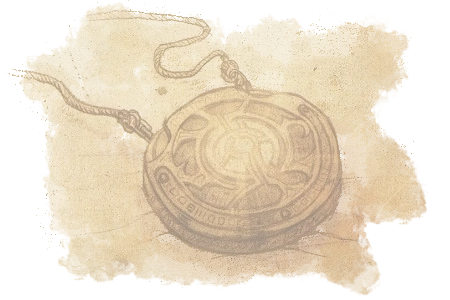
\includegraphics[width=1.75\columnwidth]{%
		images/Magic_Items/Amulet_of_Justice_background.png%
	}};%
\end{tikzpicture}%
	
\section*{Appearance}
{\entryfont The Amulet of Justice is a breathtaking artifact, its body crafted entirely from pure, lustrous silk that gleams with a subtle, otherworldly radiance. The silk is tightly woven and shaped into a smooth, flowing form that seems impossibly durable despite its delicate appearance. At the heart of the amulet rests a striking gem, as white and pristine as freshly fallen snow, radiating a soft, calming glow. The silk's edges are adorned with faint, shimmering patterns that resemble ancient runes or flowing streams, giving the amulet an aura of mystique and purpose. The white gem, seamlessly embedded in the silk, draws the eye and exudes an air of quiet, undeniable power, as if it holds the very essence of justice within its core.}

\section*{History}
{\entryfont The origins of the Amulet of Justice are steeped in mystery, its creation lost to time and whispers of forgotten lore. Tales speak of a powerful artifact forged by divine hands or ancient, unrecorded magic, though none can say for certain. What is known is that its location is a well-guarded secret, known only to an enigmatic magic-wielding blue dragon named Thaloryx, Seeker of Justice, who dwells in the craggy heights of Strathclyde. Thaloryx safeguards the knowledge of the amulet's resting place - hidden deep beneath the tranquil waters of Loch Rannoch, a place said to be warded by enchantments that deter even the boldest of seekers.}

\section*{Magic}
{\entryfont The Amulet of Justice is a powerful artifact imbued with ancient, restorative magic that serves as a counterbalance to dark forces. Its primary ability is to directly oppose and neutralize the malevolent enchantments of the infamous "Knife of Evil." When activated, the amulet emits a radiant light that pierces through shadows of corruption, unraveling the sinister spells cast by the blade. This power allows it to reverse curses, dispel harmful effects, and mend the damage wrought by the knife's influence. The amulet's magic is precise, targeting the specific threads of evil magic and restoring balance and purity to those afflicted. It is said that the gem at its center glows brighter when its restorative magic is in use, embodying the unwavering light of justice triumphing over darkness.}

\subsection*{Gameplay Mechanics}
{\entryfont While attuned to the Amulet of Justice, the wearer is shielded from the curse of the Knife of Evil, and any curses already affecting the wearer are ended and has advantage on saving throws against being frightened or charmed. Additionally, while attuned, the wearer can use an action to touch a willing creature. The touched creature must succeed on a DC 20 Wisdom saving throw (DC 15 if the wearer has reached level 10). On a success, any curse affecting the creature is suppressed until the end of their next turn. This suppression also applies to the Charmed and Frightened conditions.

If the creature succeeds on the saving throw, they can repeat the Wisdom saving throw at the end of each of their turns to extend the effect for one additional turn. Only one creature can benefit from this effect at a time (this limit increases to two creatures at 5th level, three creatures at 11th level, and four creatures at 17th level).}
\ItemCategory{}
\ItemSubCategory{}
\ItemFolder{}

\chapter*{Hammer of Glory}\stepcounter{chapter}\phantomsection\addcontentsline{toc}{chapter}{Hammer of Glory}
\itemDescriptionAndImage{Wondrous Warhammer, legendary (requires attunement by a Class-Lvl 3+ Barbarian or Fighter)}{images/Magic_Items/Hammer_of_Glory.png}{6cm}\\

\begin{tikzpicture}[remember picture, overlay]%
	\node[xshift=0.55\columnwidth, yshift=-0.35\paperheight] at (current page.center) {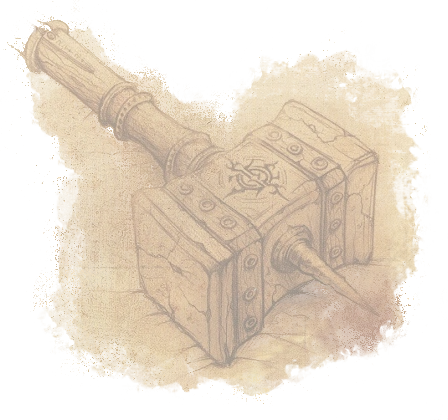
\includegraphics[width=1.3\columnwidth]{%
		images/Magic_Items/Hammer_of_Glory_background.png%
	}};%
\end{tikzpicture}%
	
\section*{Appearance}
{\entryfont The Hammer of Glory is a magnificent artifact, its design radiating both power and elegance. The head is crafted from a mysterious material described in legend as a "crystal enchantment of steel." This silvery-gray metal shimmers with a faint iridescence, occasionally catching the light in soft hues of blue. Its surface is adorned with glowing runes and intricate patterns, pulsing faintly as if alive with hidden magic.

The handle is formed from ancient dark wood, its grain polished smooth with age, reinforced by intricately engraved golden bands that add both strength and beauty. Balanced and proportional, the hammer feels both ceremonial and deadly, crafted for a hero of unmatched purpose. Surrounding it is a faint, golden aura, imbuing the artifact with a quiet majesty that commands reverence. Its presence exudes a restrained power, hinting at its potential to shape both battle and destiny.}

\section*{History}
{\entryfont The Hammer of Glory is one of the legendary Three Relics of Legends, an extraordinary trio of artifacts that includes the Knife of Evil and the Vorpal Laserblaster of Pittenweem. Crafted eons ago by the enigmatic Starlords, these relics were forged to combat an ancient, unknowable evil that threatened the cosmos in the year 10,000 BD.

Wielded during this monumental conflict, the Hammer of Glory became a symbol of defiance and hope, its power instrumental in turning the tide of battle. Once the evil was vanquished, the Starlords, fearing the potential misuse of the relics, made the decision to hide them away. The Hammer of Glory was concealed on Earth, buried deep within the rugged Cairngorm Mountains in what is now Scotland.

To this day, the Hammer of Glory remains hidden, its exact location a mystery. No map or record was left behind, and the Starlords ensured that its resting place would be inaccessible to any but the most determined and worthy.}

\section*{Magic}
{\entryfont The Hammer of Glory is a weapon of unparalleled power, its magic fueled by raw solar energy. The artifact seems to draw strength directly from the sun, radiating an intense, golden light that grows stronger when bathed in sunlight. This celestial energy not only enhances the hammer's durability and destructive force but also imbues it with a radiant aura that inspires allies and strikes fear into foes.

Only a warrior "with a heart pure of steel" can wield the Hammer of Glory. This enigmatic requirement speaks to both moral integrity and unshakable resolve, rejecting any who lack the strength of spirit or character necessary to command its immense power. To its chosen wielder, the hammer grants the ability to kill even immortal beings, severing their existence in defiance of natural or supernatural laws.

The Hammer of Glory also channels its wielder's fury into devastating enchantments. When its power is unleashed, it can focus this wrath into a concussive force that causes enemies' heads to "explode with fury", an effect both terrifying and unstoppable.}

\subsection*{Gameplay Mechanics}
{\entryfont Attacks made with the Hammer of Glory count as magical for the purpose of overcoming resistance and immunity to nonmagical attacks and damage.

Starting at 5th level, the Hammer of Glory gains a magical enchantment, granting a +1 bonus to attack rolls, damage rolls, and the DC of its magical effects. This bonus increases to +2 at 11th level and +3 at 17th level.

The Hammer of Glory has a maximum of 3 charges and when attuned to it you can use the following actions.
\begin{itemize}
	\item As an action, you can expend 1 charge to channel the hammer's power in a concussive wave of force. Each creature of your choice within a 5-foot radius must succeed on a Dexterity saving throw or take 1d6 force damage. On a success the creature takes half the amount. The saving throw DC is calculated as follows:\\

	{\centering\textbf{DC = 8 + your proficiency bonus + your Strength modifier}}

	\hfill\\The damage increases to 2d6 at 5th level, 3d6 and the radius increases to 10 feet at 11th level, and 4d6 at 17th level.

	\item You can expend 3 charges as an action to shatter a Wall of Force as if using the disintegrate spell.
\end{itemize}
\noindent When you reach 5th level the number of charges increase to 5, 7 charges at 11th level, and 10 charges at 17th level. The hammer regains all expended charges at dawn.}
	\blankpart{Resources}% Name of Act
	{}% Background Picture
	{0cm}% X-Shift
	{0cm}% Y-Shift
	{height=\paperheight}% Graphics-Options (height, width)
	{Act01}% Short-Handle
	{test}% URL
	{test}%	Image-Name
	{test}%	Artist

\onecolumn	
\chapter*{Royal Invitation}\phantomsection\addcontentsline{toc}{chapter}{Royal Invitation}
\begin{tikzpicture}[overlay, remember picture, inner sep=0pt, outer sep=0pt, path fading=fade down]%
	\node[anchor=south west, xshift=0.08\paperwidth, yshift=0.06\paperheight] at (current page.south west) {%
		\begin{minipage}{0.84\paperwidth}%
        	\centering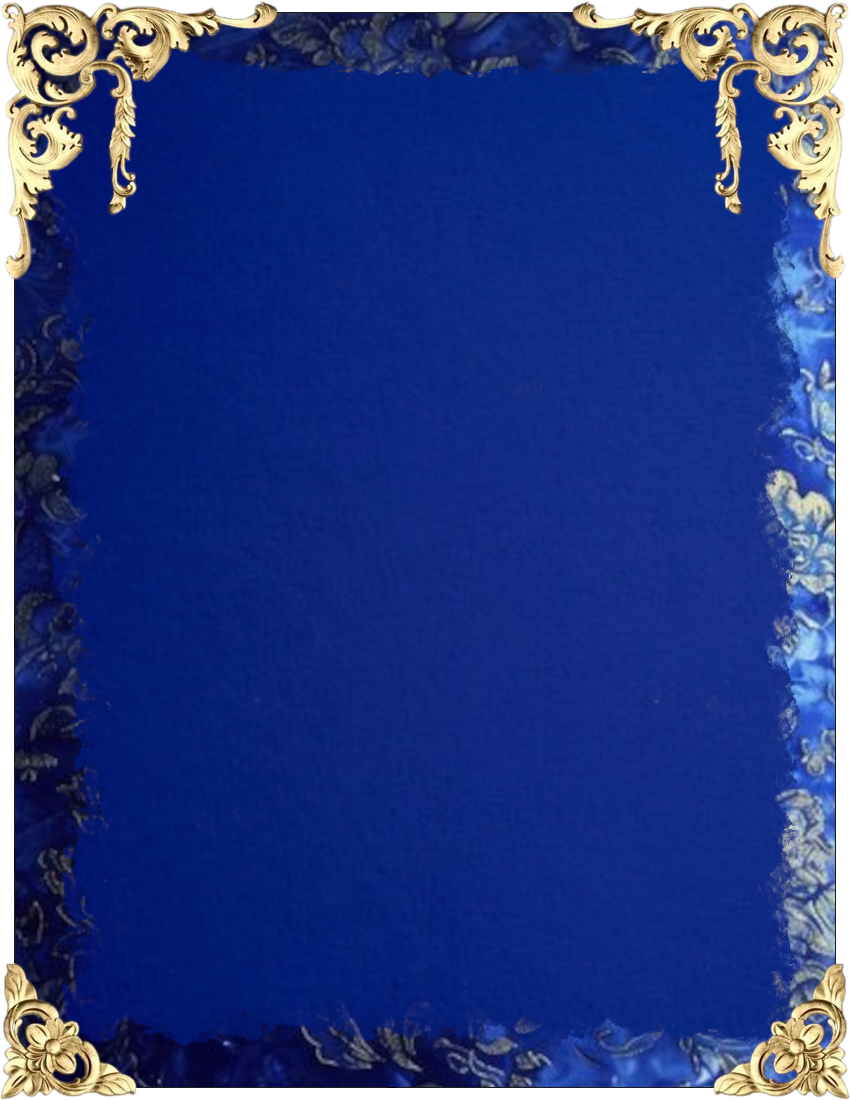
\includegraphics[width=0.84\paperwidth]{backgrounds/Royal-Invitation}%
      	\end{minipage}%
	};%
\end{tikzpicture}%
{\centering%
	\vspace*{1cm}\hfill\\%
	
\includegraphics[height=3cm,keepaspectratio]{../images/Gloryhammer_Coat_of_Arms-gold}\\
	{\darkcrystalfont\color{white}%
		{\LARGE KING DUNDAX \RoyalRoman{XIII}\\\hfill\\}%
		{\large TOGETHER WITH\\\hfill\\}%
		{\LARGE SER PROLETIUS\\\hfill\\}%
		{\large REQUEST THE HONOUR OF YOUR PRESENCE\\TO CELEBRATE THE MARRIAGE OF}%
	}%
	\vspace*{0.6cm}\hfill\\%
	{\fontsize{40}{40}\selectfont\newspaperFancyHeaderFont\color{titlegold} Prince Angus McFife\\\&\\Lady Iona McDougall\\}%
	\vspace*{0.8cm}\hfill\\%
	{\large\darkcrystalfont\color{white}May the union\\serve as a beacon of hope, courage, and unity to the\\Kingdom of Fife and beyond.}\\%
	\vspace*{0.75cm}\hfill\\%
	{\Large\darkcrystalfont\color{white}All Hail to Dundee and Crail!}\\%
	
\includegraphics[height=3cm,keepaspectratio]{../images/Gloryhammer_Coat_of_Arms-gold}\\%
}%

\onecolumn
\chapter*{Character Statblocks}\phantomsection\addcontentsline{toc}{chapter}{Character Statblocks}
\section*{Angus McFife}\phantomsection\addcontentsline{toc}{section}{Angus McFife}\label{char:AngusMcFife}%
\begin{tikzpicture}[remember picture, overlay]%
	\node[xshift=0.4\columnwidth, yshift=0.29\paperheight] at (current page.center) {\includegraphics[width=0.35\columnwidth]{%
		images/Characters/Angus_McFife%
	}};%
\end{tikzpicture}%
\vspace*{-2.4\fontdimen6\font}\hfill\\\begin{multicols}{2}%
	{\noindent\entryfont Prince Angus McFife I stands just over six feet tall, his posture regal yet relaxed, as if he'd rather be wandering the emerald hills of Fife than presiding over court. Clear blue eyes - reflecting both compassion and resolute courage - scan his surroundings constantly, ever alert for his people or a creature in need. He favours a studded leather armour of deep forest green, embroidered with silver filigree.

	Born the eldest son of King Dundax \RoyalRoman{XIII}, Angus was raised in princely halls of Dundee but still keep his humility and kindness towards the people of Fife. His voice is warm and low, each word chosen with gentle precision; when he laughs - a rich, infectious sound - it feels like sunlight breaking through canopy leaves.

	On the battlefield, Angus takes his place at the vanguard, sword aloft and voice carrying above clashing steel. His keen tactical mind discerns enemy\\weaknesses and with an\\incomparable commanding\\presence, he bolsters his\\forces' fortitude and\\resilience.\\\vspace*{-2.5\fontdimen6\font}}
	\begin{DndComment}{Playing Angus McFife}
		When portraying Prince Angus McFife I, lean into his compassionate nature. Speak with a soft, calm tone and allow him to interrupt formalities if he senses distress. Showcase his humility by having him downplay compliments and share credit with others. In moments of conflict, shift seamlessly from gentle peacemaker to determined protector. Above all, let his kindness be his strongest weapon - one that inspires allies and tames even the most hardened hearts.
	\end{DndComment}
\end{multicols}%
\begin{DndMonster}[width=\textwidth + 8pt]{Angus McFife}
	\vspace*{-17.5pt}\begin{multicols}{2}
		\DndMonsterType{Human Fighter (Lvl 7, Battle Master), lawful good}
		
		% If you want to use commas in the key values, enclose the values in braces.
		\DndMonsterBasics[
			armor-class = {16 (Studded Leather Armor)},
			hit-points  = {\DndDice{7d10 + 14}},
			speed       = {30 ft.},
		]
		
		\renewcommand{\AbilityScoreSpacer}{~}
		\DndMonsterAbilityScores[
			str = 14,
			dex = 18,
			con = 14,
			int = 10,
			wis = 12,
			cha = 16,
		]
		
		\DndMonsterDetails[
			saving-throws = {STR +4, Con +5},
			skills = {Animal Handling +4, Acrobatics +7, History +3, Insight +4, Nature +3, Perception +4, Performance +6, Persuasion +6, Stealth +7},
			%damage-vulnerabilities = {cold},
			%damage-resistances = {bludgeoning, piercing, and slashing from nonmagical attacks},
			%damage-immunities = {poison},
			senses = {Passive Perception 14},
			%condition-immunities = {poisoned},
			languages = {Common},
			challenge = -,
			proficiency-bonus=+3
		]
		
		\DndMonsterSection{Traits}	
	    \DndMonsterAction{Musician}
	    During a Short or Long Rest Angus McFife can give up to 3 allies an Heroic Inspiration.
		
		\DndMonsterAction{Great Weapon Fighting}
		When Angus rolls damage for an attack he makes with a Melee weapon that he is holding with two hands, he can treat any 1 or 2 on a damage die as a 3. The weapon must have the Two-Handed or Versatile property to gain this benefit.
		
		\DndMonsterAction{Action Surge (1 use per SR or LR)}
		Angus McFife can take an additional action during his turn.
		
		\DndMonsterAction{Combat Superiority}
		Angus McFife has 5 Superiority Dice (d8) which he can use to do his maneuvers. He regains all expended Superiority Dice when he finishes a Short or Long Rest.
		
		\DndMonsterAction{Commanding Presence}
		When Angus McFife makes a Charisma (Intimidation, Performance, or Persuasion) check he can add one Superiority Die to the roll.
		
		\DndMonsterAction{Trip Attack}
		When Angus McFife hits a creature with an attack, he can expend a Superiority Dice and add it to the damage roll. If the target is Large or smaller, it must succeed on a Strength Saving Throw (DC 15) or be knocked prone.
		
		\DndMonsterSection{Actions}
		\DndMonsterAction{Extra Attack}
		Angus McFife can attack twice whenever he takes the Attack Action.
		
		\DndMonsterAction{Commander's Strike}
		When Angus McFife takes the Attack Action he can forego his attack to command another companion to strike. That creature takes its Reaction to make an attack, adding the Superiority Die to the attack's damage roll on a hit.
		
		\DndMonsterAttack[
			name=Scimitar,
			distance=melee, % valid options are in the set {both,melee,ranged},
			%type=weapon, %valid options are in the set {weapon,spell}
			mod=+7,
			reach=5,
			%range=20/60,
			targets=one target,
			dmg=\DndDice{1d6 + 4},
			dmg-type=slashing,
			%plus-dmg=\DndDice{1d6},
			%plus-dmg-type=poison,
			or-dmg=\DndDice{1d10 + 5},
			or-dmg-when={when used with two hands},
			extra={. When Angus McFife makes an extra attack using the Scimitar hec an do so as part of the Attack action instead of using the Bonus Action},
		]
		
		\DndMonsterAttack[
			name=Shortsword,
			distance=melee, % valid options are in the set {both,melee,ranged},
			%type=weapon, %valid options are in the set {weapon,spell}
			mod=+7,
			reach=5,
			%range=20/60,
			targets=one target,
			dmg=\DndDice{1d6 + 4},
			dmg-type=piercing,
			%plus-dmg=\DndDice{1d6},
			%plus-dmg-type=poison,
			%or-dmg=,
			%or-dmg-when=,
			extra={. When Angus hits a creature with this weapon he gains Advantage on the next attack roll against that creature},
		]
		
		\DndMonsterAttack[
			name=Longbow,
			distance=ranged, % valid options are in the set {both,melee,ranged},
			%type=weapon, %valid options are in the set {weapon,spell}
			mod=+7,
			%reach=5,
			range=150/600,
			targets=one target,
			dmg=\DndDice{1d8 + 4},
			dmg-type=piercing,
			%plus-dmg=\DndDice{1d6},
			%plus-dmg-type=poison,
			%or-dmg=,
			%or-dmg-when=,
			extra={. A creature hit with this attack has its speed reduced by 10 feet, up to a maximum reduction of 10 feet},
		]
		
		\DndMonsterSection{Bonus Action}
		\DndMonsterAction{Second Wind (3 charges)}
		Angus McFife regains \DndDice{1d10 + 7} Hit Points. Also he can move up to half his speed without provoking Opportunity Attacks.
		
		\DndMonsterAction{Rally}
	    Angus McFife bolsters the resolve of a creature. By expending one Superiority Die that creature gains \DndDice{1d8 + 3} Temporary Hit Points.
		
		\DndMonsterSection{Reaction}
		\DndMonsterAction{Riposte}
		When a creature misses Angus McFife he can expend a Superiority Die to immediately attack that creature adding the Superiority Die to the attack's damage roll on a hit.
	\end{multicols}
\end{DndMonster}%
\clearpage
\section*{The Hootsman}\phantomsection\addcontentsline{toc}{section}{Hootsman}\label{char:Hootsman}%
\begin{DndMonster}[width=\textwidth + 8pt]{Hootsman}
	\vspace*{-17.5pt}\begin{multicols}{2}
		\DndMonsterType{Warforged Barbarian (Lvl 9, Path fo the Berserker), chaotic neutral}
		
		% If you want to use commas in the key values, enclose the values in braces.
		\DndMonsterBasics[
			armor-class = {16 (Natural Armor)},
			hit-points  = {\DndDice{9d12 + 36}},
			speed       = {40 ft.},
		]
		
		\renewcommand{\AbilityScoreSpacer}{~}
		\DndMonsterAbilityScores[
			str = 20,
			dex = 14,
			con = 16,
			int = 11,
			wis = 14,
			cha = 10,
		]
		
		\DndMonsterDetails[
			saving-throws = {STR +9, CON +7},
			skills = {Animal Handling +6, Athletics +9, Intimidation +4, Nature +4, Perception +6, Survival +6},
			%damage-vulnerabilities = {cold},
			damage-resistances = {Poison},
			%damage-immunities = {poison},
			senses = {Passive Perception 16},
			condition-immunities = {disease},
			languages = {Common, Sylvan},
			challenge = -,
			proficiency-bonus=+4
		]
		
		\DndMonsterSection{Traits}
		\DndMonsterAction{Rage}
		While the Rage is active, the Hootsman gains the following benefits:
		\begin{itemize}
			\item He has resistance against bludgeoning, slashing, and piercing damage
			\item When he makes an attack using Strength, his damage increases by +3
			\item He has advantage on Strength checks and Strength saving throws
		\end{itemize}
		While in Rage, the Hootsman is also immune to the Charmed and Frightened condition and already affecting conditions of that kind end if he enters his Rage.
		Additionally, the Hootsman can make any checks of the following skills as a Strength check: Acrobatics, Intimidation, Perception, Stealth, and Survival.
		
		\DndMonsterAction{Feral Instinct}
		The Hootsman has advantage on Initiative Rolls.
		
		\DndMonsterAction{Reckless Attack}
		When the Hootsman makes his first attack roll he can give himself Advantage on it until the next turn, but attack rolls against him have Advantage during that time.
		He can forego the Advantage to deal an additional \DndDice{1d10} damage and either push the target 15 feet and move up to half his Speed towards the target without provoking Opportunity Attacks or reduce the targets speed by 15 feet.
		If the Hootsman's Rage is active when using this trait the target also takes \DndDice{3d6} additional damage of the same type as the attack.
		
		\DndMonsterSection{Actions}
		\DndMonsterAction{Extra Attack}
		The Hootsman can attack twice whenever he takes the Attack Action.
		
		\DndMonsterAttack[
			name=Battleaxe,
			distance=melee, % valid options are in the set {both,melee,ranged},
			%type=weapon, %valid options are in the set {weapon,spell}
			mod=+9,
			reach=5,
			%range=20/60,
			targets=one target,
			dmg=\DndDice{1d8 + 5},
			dmg-type=slashing,
			%plus-dmg=\DndDice{1d6},
			%plus-dmg-type=poison,
			or-dmg=\DndDice{1d10 + 5},
			or-dmg-when={when used with two hands},
			extra={. The creature hit with this attack must succeed on a DC 17 Constitution Saving Throw or is knocked prone},
		]
		
		\DndMonsterAttack[
			name=Greataxe,
			distance=melee, % valid options are in the set {both,melee,ranged},
			%type=weapon, %valid options are in the set {weapon,spell}
			mod=+9,
			reach=5,
			%range=20/60,
			targets=one target,
			dmg=\DndDice{1d12 + 5},
			dmg-type=slashing,
			%plus-dmg=\DndDice{1d6},
			%plus-dmg-type=poison,
			%or-dmg=\DndDice{1d10 + 5},
			%or-dmg-when={when used with two hands},
			extra={. Once per turn when the Hootsman hits a creature with this attack he can make another attack roll against another creature within 5 feet of the first target. On a hit the creature takes \DndDice{1d12} slashing damage},
		]
		
		\DndMonsterAttack[
			name=Longbow,
			distance=ranged, % valid options are in the set {both,melee,ranged},
			%type=weapon, %valid options are in the set {weapon,spell}
			mod=+7,
			%reach=5,
			range=150/600,
			targets=one target,
			dmg=\DndDice{1d8 + 2},
			dmg-type=piercing,
			%plus-dmg=\DndDice{1d6},
			%plus-dmg-type=poison,
			%or-dmg=\DndDice{1d10 + 5},
			%or-dmg-when={when used with two hands},
			extra={. A creature hit with this attack has its speed reduced by 10 feet, up to a maximum reduction of 10 feet},
		]
		
		\DndMonsterSection{Bonus Action}
		\DndMonsterAction{Rage (4 / Short or Long Rest)}
		The Hootsman can enter a Rage while he is not wearing Heavy Armor. He will gain all Rage benefits and it lasts until the end of his next turn if he does not extend it. He can maintain the Rage for up to 10 minutes.
	\end{multicols}
\end{DndMonster}%
\clearpage
\section*{Ser Proletius}\phantomsection\addcontentsline{toc}{section}{Ser Proletius}\label{char:SerProletius}%
\begin{DndMonster}[width=\textwidth + 8pt]{Ser Proletius}
	\vspace*{-17.5pt}\begin{multicols}{2}
		\DndMonsterType{Human Paladin (Lvl 10, Oath of the Crown), Lawful Good}
		
		% If you want to use commas in the key values, enclose the values in braces.
		\DndMonsterBasics[
			armor-class = {20 (Plate Armor, Shield)},
			initiative	= +3,
			hit-points  = {\DndDice{10d10 + 30}},
			speed       = {30 ft.},
		]
		
		\renewcommand{\AbilityScoreSpacer}{~}
		\DndMonsterAbilityScores[
			str = 20,
			dex = 9,
			con = 16,
			int = 10,
			wis = 11,
			cha = 16,
		]
		
		\DndMonsterDetails[
			saving-throws			= {WIS +4, CHA +7},
			skills					= {Athletics +6, History +4, Insight +4, Intimidation +7, Persuasion +7},
%			damage-vulnerabilities	= {Cold},
%			damage-resistances		= {Bludgeoning, Piercing, and Slashing from nonmagical attacks},
%			damage-immunities		= {Poison},
%			condition-immunities	= {Poisoned},
%			gear					= {Leather Armor, Light Crossbow, Scimitar},
			senses					= {Passive Perception 10},
			languages				= {Common},
%			challenge				= -,
			proficiency-bonus		= +4,
		]
		
		\DndMonsterSection{Traits}	
	    \DndMonsterAction{Savage Attacker}
		Once per turn when Ser Proletius hits another creature with a weapon, he can roll the weapon's damage twice and use either roll against the target.
		
		\DndMonsterAction{Channel Divinity}
		Ser Proletius has two Channel Divinity charges per Long Rest.
		
		\DndMonsterAction{Aura of Protection}
		Ser Proletius and his allies within a 10-foot radius of him gains a +3 bonus to all saving throws. Also all have Immunity to the Frightened condition while in the area of effect.
		
		\DndMonsterSection{Actions}
		\DndMonsterAction{Extra Attack}
		Ser Proletius can attack twice whenever he takes the Attack Action.
		
		\DndMonsterAttack[
			name			= Longsword,
			distance		= melee,	% valid options are in the set {both,melee,ranged}
%			type			= weapon,	% valid options are in the set {weapon,spell}
			mod				= +9,
			reach			= 5,
%			range			= 20/60,
			targets			= one target,
			dmg				= \DndDice{1d8 + 5},
			dmg-type		= Slashing,
%			plus-dmg		= \DndDice{1d6},
%			plus-dmg-type	= Poison,
			or-dmg			= \DndDice{1d10 + 5},
			or-dmg-when		= {when used with two hands},
			extra			= {. The creature hit with this attack has Disadvantage on its next attack roll before the start of Ser Proletius' next turn},
		]
		
		\DndMonsterAttack[
			name			= Javelin,
			distance		= ranged, % valid options are in the set {both,melee,ranged},
%			type			= weapon, %valid options are in the set {weapon,spell}
			mod				= +9,
%			reach			= 5,
			range			= 30/120,
			targets			= one target,
			dmg				= \DndDice{1d6 + 5},
			dmg-type		= Piercing,
%			plus-dmg		= \DndDice{1d6},
%			plus-dmg-type	= Poison,
%			or-dmg			= \DndDice{1d20},
%			or-dmg-when		= {},
			extra			= {. A creature hit with this attack has its speed reduced by 10 feet, up to a maximum reduction of 10 feet},
		]
		
		\DndMonsterSection{Spells}
		\begin{DndMonsterSpells}
			\item[Spellcasting] Ser Proletius is a 10th-level spellcaster. His spellcasting ability is Charisma (spell save DC 15, +7 to hit with spell attacks). Ser Proletius has the following paladin spells prepared:
			\DndInnateSpellLevel[1]{Aura of Vitality, Command, Compelled Duel, Divine Smite, Find Steed, Spirit Guardians, Warding Bond, Zone of Truth}
			\DndMonsterSpellLevel[1][4]{Bless, Command, Compelled Duel, Divine Smite, Heroism, Shield of Faith}
			\DndMonsterSpellLevel[2][3]{Aid, Branding Smite, Find Steed, Prayer of Healing, Warding Bond, Zone of Truth}
			\DndMonsterSpellLevel[3][2]{Aura of Vitality, Crusader's Mantle, Revivify, Spirit Guardians}
		\end{DndMonsterSpells}
		
		\DndMonsterSection{Bonus Action}
		\DndMonsterAction{Lay on Hands}
		Ser Proletius can touch a creature and draw power from the pool of healing (50 points) to restore a number of Hit Points to that creature.
		
		He can also expend 5 Hit Points from the pool to remove the Poisoned condition from that creature
		
		\DndMonsterAction{Divine Sense}
		Ser Proletius can use a Channel Divinity charge and open his awareness to detect Celestials, Fiends, and Undead within 60 feet of himself. Additionally, within the same radius he can also detect the presence of any place or object that has been consecrated or desecrated, as with the Hallow spell.
		
		\DndMonsterAction{Champion Challenge}
		Ser Proletius can use a Channel Divinity charge to compel other creatures to battle with him. Each creature of his choice within 30 feet must make a Wisdom saving throw. On a failed save a creature cannot willingly move more than 30 feet away from him. The condition ends if Ser Proletius is incapacitated or the creature is more than 30 feet away from him.
		
		\DndMonsterAction{Champion Challenge}
		Ser Proletius can use a Channel Divinity charge to bolster injured creatures. Each creature within 30 feet regains \DndDice{1d6 + 3} Hit Points if it has no more than half of its Hit Points.
		
		\DndMonsterSection{Reaction}
		\DndMonsterAction{Interception}
		When Ser Proletius sees a creature hit another creature within 5 feet of him with an attack roll, he can reduce the damage by \DndDice{1d10 + 4}.
		
		\DndMonsterAction{Divine Allegiance}
		If a creature within 5 feet of Ser Proletius takes damage, he can use his reaction to magically substitute his own health for that of the target creature, causing that creature not to take the damage. Instead, Ser Proletius takes the damage. This damage to him can't be reduced or prevented in any way.
	\end{multicols}
\end{DndMonster}%
\clearpage
\section*{Zargothrax}\phantomsection\addcontentsline{toc}{section}{Zargothrax}\label{char:Zargothrax}%
\vspace*{-2.4\fontdimen6\font}\hfill\\\begin{multicols}{2}%
	{\noindent\entryfont Lorem ipsum dolor sit amet, consectetur adipiscing elit, sed do eiusmod tempor incididunt ut labore et dolore magna aliqua. Nullam eget felis eget nunc lobortis mattis aliquam faucibus. Dictumst quisque sagittis purus sit. Mattis nunc sed blandit libero volutpat sed cras ornare. Blandit cursus risus at ultrices mi tempus imperdiet. Et netus et malesuada fames ac turpis egestas maecenas. Nibh cras pulvinar mattis nunc sed blandit. Varius vel pharetra vel turpis nunc eget lorem dolor. Tellus orci ac auctor augue. Nulla aliquet enim tortor at auctor urna nunc id cursus. A condimentum vitae sapien pellentesque habitant morbi tristique. Viverra suspendisse potenti nullam ac tortor. Quam lacus suspendisse faucibus interdum posuere lorem ipsum dolor. Nisl condimentum id venenatis a. Dui nunc mattis enim ut tellus elementum sagittis.}
\end{multicols}%
\begin{DndMonster}[width=\textwidth + 8pt]{Zargothrax} % Acererak
	\vspace*{-17.5pt}\begin{multicols}{2}
		\DndMonsterType{Medium Undead, Chaotic Evil}
		
		% If you want to use commas in the key values, enclose the values in braces.
		\DndMonsterBasics[
			armor-class = {21 (Natural Armor)},
			initiative	= +3,
			hit-points  = {\DndDice{30d8 + 150}},
			speed       = {30 ft.},
		]
		
		\renewcommand{\AbilityScoreSpacer}{~}
		\DndMonsterAbilityScores[
			str = 13,
			dex = 16,
			con = 20,
			int = 27,
			wis = 21,
			cha = 20,
		]
		
		\DndMonsterDetails[
			%saving-throws			= {CON +8, CHA +9},
			skills					= {Arcana +22, History +22, Insight +12. Perception +12},
			%damage-vulnerabilities	= {cold},
			damage-resistances		= {Cold, Lightning},
			damage-immunities		= {Bludgeoning, Piercing, and Slashing damage from nonmagical attack, Necrotic, Poison},
			condition-immunities	= {Blinded, Charmed, Deafened, Exhaustion, Frightened, Paralyzed, Petrified, Poisoned, Stunned},
%			gear					= {Leather Armor, Light Crossbow, Scimitar},
			senses					= {Truesight 120 ft., Passive Perception 22},
			languages				= {Abyssal, Common, Draconic, Dwarvish, Elvish, Giant, Infernal, Primordial, Undercommon},
			challenge				= 23,
			proficiency-bonus		= +7,
		]
		
		\DndMonsterSection{Traits}
		\DndMonsterAction{Legendary Resistance (3/Day)}
		If Zargothrax fails a saving throw, he can choose to succeed instead.
		
		\DndMonsterAction{Turn Resistance}
		Zargothrax has advantage on saving throws against any effect that turns undead.
		
		\DndMonsterSection{Actions}
		\DndMonsterAttack[
			name			= Knife of Evil,
			distance		= melee,	% valid options are in the set {both,melee,ranged}
			%type			= weapon,	% valid options are in the set {weapon,spell}
			mod				= +11,
			reach			= 5,
			%range			= 20/60,
			targets			= one target,
			dmg				= \DndDice{1d4 + 4},
			dmg-type		= Piercing,
			%plus-dmg		= \DndDice{1d6},
			%plus-dmg-type	= Poison,
			%or-dmg			= \DndDice{1d20},
			%or-dmg-when	= {},
			%extra			= {},
		]
		
		\DndMonsterAttack[
			name			= Paralyzing Touch,
			distance		= melee,	% valid options are in the set {both,melee,ranged}
			type			= spell,	% valid options are in the set {weapon,spell}
			mod				= +15,
			reach			= 5,
%			range			= 20/60,
			targets			= one target,
			dmg				= \DndDice{3d6},
			dmg-type		= Cold,
%			plus-dmg		= \DndDice{1d6},
%			plus-dmg-type	= Poison,
%			or-dmg			= \DndDice{1d20},
%			or-dmg-when		= {},
			extra			= {, and the target must succeed on a DC 20 Constitution saving throw or be paralyzed for 1 minute. The target can repeat the saving throw at the end of each of its turns, ending the effect on itself on a success},
		]
		
		\DndMonsterSection{Spells}
		\begin{DndMonsterSpells}
			\item[Spellcasting] Zargothrax is a 20th-level spellcaster. His spellcasting ability is Intelligence (spell save DC 23, +15 to hit with spell attacks). Zargothrax has the following wizard spells prepared:
			\DndMonsterSpellLevel[Cantrips][At will]{Mage Hand, Ray of Frost, Shocking Grasp}
			\DndMonsterSpellLevel[1][At will]{Ray of Sickness, Shield}
			\DndMonsterSpellLevel[2][At will]{Arcane Lock, Knock}
			\DndMonsterSpellLevel[3][At will]{Animate Dead, Counterspell}
			\DndMonsterSpellLevel[4][3]{Blight, Ice Storm, Phantasmal Killer}
			\DndMonsterSpellLevel[5][3]{Cloudkill, Hold Monster, Wall of Force}
			\DndMonsterSpellLevel[6][3]{Chain Lightning, Circle of Death, Disintegrate}
			\DndMonsterSpellLevel[7][3]{Finger of Death, Plane Shift, Teleport}
			\DndMonsterSpellLevel[8][2]{Maze, Mind Blank}
			\DndMonsterSpellLevel[9][2]{Power Word Kill, Time Stop}
		\end{DndMonsterSpells}
		
		\DndMonsterSection{Legendary Actions}
		Zargothrax can take 3 legendary actions, choosing from the options below. Only one legendary action can be used at a time and only at the end of another creature's turn. Zargothrax regains spent legendary actions at the start of its turn.
		\begin{DndMonsterLegendaryActions}
			\DndMonsterLegendaryAction{At-Will Spell}{Zargothrax cast one of his at-will spells.}
			\DndMonsterLegendaryAction{Melee Attack}{Zargothrax uses Paralyzing Touch or makes one melee attack with his Knife of Evil.}
			\DndMonsterLegendaryAction{Frightening Gaze (Costs 2 Actions)}{Zargothrax fixes his gaze on one creature he can see within 10 feet of him. The target must succeed on a DC 20 Wisdom saving throw against this magic or become frightened for 1 minute. The frightened target can repeat the saving throw at the end of each of its turns, ending the effect on itself on a success. If a target's saving throw is successful or the effect ends for it, the target its immune to Zargothrax's gaze for the next 24 hours.}
			\DndMonsterLegendaryAction{Disrupt Life (Costs 3 Actions)}{Each creature within 20 feet of Zargothrax must make a DC 20 Constitution saving throw against this magic, taking 42 (12d6) necrotic damage on a failed save, or half as much damage on a successful one.}
		\end{DndMonsterLegendaryActions}
	\end{multicols}
\end{DndMonster}%
\twocolumn
\clearpage
\section*{Tourney Contestants}\phantomsection\addcontentsline{toc}{section}{Tourney Contestants}%
\subsection{Alasdair MacLeod}\label{char:AlasdairMacLeod}
{\entryfont Alasdair MacLeod hails from the rugged slopes of the Glencoe Mountains, where his Stone-Goliath clan tests their mettle by hurling ancient granite boulders off towering cliffs. He enters Dundee's wedding tourney not for mere sport, but to prove that his people's hard-won strength from the Highlands still commands respect across Caledonia.}
\begin{DndMonster}[width=0.5\textwidth]{Alasdair MacLeod}
	\DndMonsterType{Goliath (Stone) Barbarian, Neutral}
	
	% If you want to use commas in the key values, enclose the values in braces.
	\DndMonsterBasics[
		armor-class = {16 (Natural Armor)},
		initiative	= +1,
		hit-points  = {\DndDice{1d12 + 4}},
		speed       = {35 ft.},
	]
	
	\renewcommand{\AbilityScoreSpacer}{~}
	\DndMonsterAbilityScores[
		str = 18,
		dex = 13,
		con = 15,
		int = 10,
		wis = 12,
		cha = 8,
	]
	
	\DndMonsterDetails[
		saving-throws			= {STR +6, CON +4},
		skills					= {Athletics +6, Animal Handling +3, Survival +3},
%		damage-vulnerabilities	= {Cold},
%		damage-resistances		= {Bludgeoning, Piercing, and Slashing from nonmagical attacks},
%		damage-immunities		= {Poison},
%		condition-immunities	= {Poisoned},
%		gear					= {Leather Armor, Light Crossbow, Scimitar},
		senses					= {Passive Perception 11},
		languages				= {Common, Giant},
%		challenge				= -,
%		proficiency-bonus		= +2,
	]
    
	\DndMonsterSection{Traits}
	\DndMonsterAction{Powerful Build}
	Alasdair has Advantage on any saving throw he makes to end the Grappled condition. He also counts as one size larger when determining his carrying capacity.
	
	\DndMonsterAction{Rage}
	While the Rage is active, Alasdair gains the following benefits:
	\begin{itemize}
		\item He has resistance against bludgeoning, slashing, and piercing damage
		\item When he makes an attack using Strength, his damage increases by +2
		\item He has advantage on Strength checks and Strength saving throws
	\end{itemize}
	
	\DndMonsterSection{Actions}
	\DndMonsterAttack[
		name			= Battleaxe,
		distance		= melee,	% valid options are in the set {both,melee,ranged}
%		type			= weapon,	% valid options are in the set {weapon,spell}
		mod				= +6,
		reach			= 5,
%		range			= 20/60,
		targets			= one target,
		dmg				= \DndDice{1d8 + 4},
		dmg-type		= Slashing,
%		plus-dmg		= \DndDice{1d6},
%		plus-dmg-type	= Poison,
		or-dmg			= \DndDice{1d10 + 4},
		or-dmg-when		= {when used with two hands},
%		extra			= {},
	]
	
	\DndMonsterAttack[
		name			= Shortbow,
		distance		= ranged,	% valid options are in the set {both,melee,ranged}
%		type			= weapon,	% valid options are in the set {weapon,spell}
		mod				= +3,
%		reach			= 5,
		range			= 80/320,
		targets			= one target,
		dmg				= \DndDice{1d6 + 1},
		dmg-type		= Piercing,
%		plus-dmg		= \DndDice{1d6},
%		plus-dmg-type	= Poison,
%		or-dmg			= \DndDice{1d20},
%		or-dmg-when		= {},
%		extra			= {},
	]
	
	\DndMonsterSection{Bonus Actions}
	\DndMonsterAction{Rage (2 / Short or Long Rest)}
	Alasdair can enter a Rage while he is not wearing Heavy Armor. He will gain all Rage benefits and it lasts until the end of his next turn if he does not extend it. He can maintain the Rage for up to 10 minutes.
	
	\DndMonsterSection{Reactions}
	\DndMonsterAction{Stone's Endurance (2 / Long Rest)}
    When Alasdair takes damage, he can take a Reaction to roll 1d12. Add his Constitution modifier to the number rolled and reduce the damage by the total.
\end{DndMonster}
\vfill\eject
\subsection{Ewan MacRae of Dunkeld}\label{char:EwanMacRae}
{\entryfont Ewan MacRae stands as Dunkeld's unyielding bulwark, born and raised on the misty banks of the River Tay where he learned swordplay guarding abbey walls and herding cattle through Highland glens. Clad in steel plate etched with the symbol of Dunkeld's fallen heroes, he has repelled raiders and settled feuds with unshakeable discipline. Now, as the clear favourite of Dundee's wedding tourney, Ewan seeks not only personal glory but to elevate his town's renown - victory would cement Dunkeld's reputation as a bastion of strength and honour throughout Scotland.}
\begin{DndMonster}[width=0.5\textwidth]{Ewan MacRae}
	\DndMonsterType{Human Fighter, Lawful Good}
	
	% If you want to use commas in the key values, enclose the values in braces.
	\DndMonsterBasics[
		armor-class = {17 (Splint Mail)},
		initiative	= +4,
		hit-points  = {\DndDice{4d10 + 8}},
		speed       = {30 ft.},
	]
	
	\renewcommand{\AbilityScoreSpacer}{~}
	\DndMonsterAbilityScores[
		str = 18,
		dex = 18,
		con = 15,
		int = 8,
		wis = 13,
		cha = 14,
	]
	
	\DndMonsterDetails[
		saving-throws			= {STR +6, CON +4},
		skills					= {Athletics +6, Animal Handling +3, Perception +3},
%		damage-vulnerabilities	= {Cold},
%		damage-resistances		= {Bludgeoning, Piercing, and Slashing from nonmagical attacks},
%		damage-immunities		= {Poison},
%		condition-immunities	= {Poisoned},
%		gear					= {Leather Armor, Light Crossbow, Scimitar},
		senses					= {Passive Perception 13},
		languages				= {Common},
%		challenge				= -,
%		proficiency-bonus		= +2,
	]
	
	\DndMonsterSection{Traits}
    \DndMonsterAction{Savage Attacker}
    Once per turn when Ewan hits another creature with a weapon, he can roll the weapon's damage twice and use either roll against the target.
    
	\DndMonsterAction{Great Weapon Fighting}
	When Ewan rolls damage for an attack he makes with a Melee weapon that he is holding with two hands, he can treat any 1 or 2 on a damage die as a 3. The weapon must have the Two-Handed or Versatile property to gain this benefit.
	
	\DndMonsterAction{Action Surge (1 / Short or Long Rest)}
    Ewan takes one additional Action.
	
	\DndMonsterAction{Improved Critical}
	Ewan's attack rolls with weapons and Unarmed Strikes can score a Critical Hit on a roll of 19 or 20 on the d20.
	
	\DndMonsterAction{Remarkable Athlete}
	Thanks to Ewan's athleticism, Ewan has Advantage on Initiative rolls and Strength (Athletics) checks.\\
	In addition, immediately after he scores a Critical Hit, he can move up to half his Speed without provoking Opportunity Attacks.
	
	\DndMonsterSection{Actions}	
	\DndMonsterAttack[
		name			= Greatsword,
		distance		= melee,	% valid options are in the set {both,melee,ranged}
%		type			= weapon,	% valid options are in the set {weapon,spell}
		mod				= +6,
		reach			= 5,
%		range			= 20/60,
		targets			= one target,
		dmg				= \DndDice{2d6 + 4},
		dmg-type		= Slashing,
%		plus-dmg		= \DndDice{1d6},
%		plus-dmg-type	= Poison,
%		or-dmg			= \DndDice{1d20},
%		or-dmg-when		= {},
%		extra			= {},
	]
	
	\DndMonsterAttack[
		name			= Shortbow,
		distance		= ranged,	% valid options are in the set {both,melee,ranged}
%		type			= weapon,	% valid options are in the set {weapon,spell}
		mod				= +7,
%		reach			= 5,
		range			= 80/320,
		targets			= one target,
		dmg				= \DndDice{1d6 + 3},
		dmg-type		= Piercing,
%		plus-dmg		= \DndDice{1d6},
%		plus-dmg-type	= Poison,
%		or-dmg			= \DndDice{1d20},
%		or-dmg-when		= {},
%		extra			= {},
	]
	
	\DndMonsterSection{Bonus Action}
	\DndMonsterAction{Second Wind (1 / Short or Long Rest)}
	Ewan regains \DndDice{1d10 + 4} Hit Points.
\end{DndMonster}
\vfill\eject
\subsection{Gavin Buchanan}\label{char:GavinBuchanan}
{\entryfont Gavin Buchanan is a nimble halfling rogue from Dundee's bustling harbour district, where he learned to ghost through alleyways and lift purses with a rakish grin. His keen green eyes spot every coin pouch and councilor's secret, and his leather jerkin hides tools for any trick. In the wedding tourney, he aims to prove that wit and speed can outmatch steel - and maybe pocket a few unexpected prizes along the way.}
\begin{DndMonster}[width=0.5\textwidth]{Gavin Buchanan}
	\DndMonsterType{Halfling Rogue, chaotic neutral}
	
	% If you want to use commas in the key values, enclose the values in braces.
	\DndMonsterBasics[
		armor-class = {15 (Leather Armor)},
		hit-points  = {\DndDice{2d10 + 4}},
		speed       = {30 ft.},
	]
	
	\renewcommand{\AbilityScoreSpacer}{~}
	\DndMonsterAbilityScores[
		str = 9,
		dex = 18,
		con = 14,
		int = 15,
		wis = 13,
		cha = 12,
	]
	
	\DndMonsterDetails[
		saving-throws = {DEX +6, INT +4},
		skills = {Acrobatics +6, Perception +5, Stealth +8},
		%damage-vulnerabilities = {cold},
		%damage-resistances = {bludgeoning, piercing, and slashing from nonmagical attacks},
		%damage-immunities = {poison},
		senses = {Passive Perception 15},
		%condition-immunities = {poisoned},
		languages = {Common, Thieves' Cant},
		challenge = 1/2,
	]
    
	\DndMonsterSection{Traits}
	\DndMonsterAction{Brave}
	Gavin has Advantage on saving throws he makes to avoid or end the Frightened condition.
	
	\DndMonsterAction{Halfling Nimbleness}
	Gavin can move through the space of any creature that is a size larger than him, but he can't stop in the same space.
	
	\DndMonsterAction{Luck}
	When Gavin rolls a 1 on the d20 of a D20 Test, he can reroll the die, and he must use the new roll.
	
	\DndMonsterAction{Naturally Stealthy}
	Gavin can take the Hide action even when he is obscured only by a creature that is at least one size larger than him.
	
	\DndMonsterAction{Sneak Attack}
	Once per turn, Gavin can deal an extra 2d6 damage to one creature he hits with an attack roll if he has Advantage on the roll and the attack uses a Finesse or Ranged weapon. The extra damage's tyoe is the same as the weapon's type.
	
	\DndMonsterSection{Actions}
	\DndMonsterAttack[
		name=Dagger,
		distance=melee, % valid options are in the set {both,melee,ranged},
		%type=weapon, %valid options are in the set {weapon,spell}
		mod=+6,
		reach=5,
		%range=20/60,
		targets=one target,
		dmg=\DndDice{1d4 + 4},
		dmg-type=piercing,
		%plus-dmg=\DndDice{1d6},
		%plus-dmg-type=poison,
		%or-dmg=,
		%or-dmg-when={when used with two hands},
		%extra={},
	]
	
	\DndMonsterAttack[
		name=Shortbow,
		distance=ranged, % valid options are in the set {both,melee,ranged},
		%type=weapon, %valid options are in the set {weapon,spell}
		mod=+6,
		%reach=5,
		range=80/320,
		targets=one target,
		dmg=\DndDice{1d6 + 4},
		dmg-type=piercing,
		%plus-dmg=\DndDice{1d6},
		%plus-dmg-type=poison,
		%or-dmg=,
		%or-dmg-when=,
		%extra={},
	]
	
	\begin{DndMonsterSpells}
		\item[Spellcasting] Gavin Buchanan can cast the following spells using Intelligence as the spellcasting ability (spell save DC 12, +4 to hit with spell attacks):
		\DndInnateSpellLevel{Mage Hand, Mind Sliver, Minor Illusion}
		\DndMonsterSpellLevel[1][2]{Disguise Self, Fog Cloud, Long Strider}
	\end{DndMonsterSpells}
	
	\DndMonsterSection{Bonus Actions}
	\DndMonsterAction{Cunning Action}
	Gavin can take one of the following actions as a Bonus Action: Dash, Disengage, or Hide.
	
	\DndMonsterAction{Steady Aim}
	If Gavin hasn't moved during his turn, he can give himself Advantage on his next attack on the current turn. After he uses it, his Speed is 0 until the end of the current turn.
\end{DndMonster}
\vfill\eject
\subsection{Hamish "Halfwit" McGregor}\label{char:HamishMcGregor}
{\entryfont Hamish "Halfwit" McGregor strides into the lists as Dundee's most infamous human bard, lute slung crooked over one shoulder and mismatched armour clinking with every off-key chord. Hailing from the city's poorest quarter, his performances are as chaotic as his swordplay - he mangles melodies, forgets lyrics, and somehow still manages to rally a crowd's laughter. Nobody's quite sure how he earned a spot in the wedding tourney - some say it's for sheer entertainment - but Hamish embraces the role, blundering through verse and verse until even his foes can't help but chuckle at his well-meaning, bumbling charm.}
\begin{DndMonster}[width=0.5\textwidth]{Hamish McGregor}
	\DndMonsterType{Human Bard, Chaotic Good}
	
	% If you want to use commas in the key values, enclose the values in braces.
	\DndMonsterBasics[
		armor-class = {9 (Leather Armor)},
		initiative	= -2,
		hit-points  = {\DndDice{1d8 + 2}},
		speed       = {30 ft.},
	]
	
	\renewcommand{\AbilityScoreSpacer}{~}
	\DndMonsterAbilityScores[
		str = 7,
		dex = 7,
		con = 14,
		int = 8,
		wis = 14,
		cha = 20,
	]
	
	\DndMonsterDetails[
		saving-throws			= {DEX +0, CHA +7},
		skills					= {Acrobatics +0, Performance +7, Survival +4},
%		damage-vulnerabilities	= {Cold},
%		damage-resistances		= {Bludgeoning, Piercing, and Slashing from nonmagical attacks},
%		damage-immunities		= {Poison},
%		condition-immunities	= {Poisoned},
%		gear					= {Leather Armor, Light Crossbow, Scimitar},
		senses					= {Passive Perception 12},
		languages				= {Common},
%		challenge				= -,
%		proficiency-bonus		= +2,
	]
	
	\DndMonsterSection{Traits}
    \DndMonsterAction{Lucky (2 / Long Rest)}
    Hamish can expend one use of his Lucky Trait to give himself Advantage whenever he rolls a d20 for a D20 test. He can also expend a use to give another creature Disadvantage on its next attack roll against him.
    
	\DndMonsterAction{Encouraging Song}
	Whenever Hamish finishes a Short or Long Rest he can use an instrument he is proficient with and give Heroic Inspiration to up to 2 allies that can hear the song.
	
	\DndMonsterSection{Actions}
	\DndMonsterAttack[
		name			= Dagger,
		distance		= melee,	% valid options are in the set {both,melee,ranged}
%		type			= weapon,	% valid options are in the set {weapon,spell}
		mod				= +0,
		reach			= 5,
%		range			= 20/60,
		targets			= one target,
		dmg				= \DndDice{1d4 - 2},
		dmg-type		= Slashing,
%		plus-dmg		= \DndDice{1d6},
%		plus-dmg-type	= Poison,
%		or-dmg			= \DndDice{1d20},
%		or-dmg-when		= {},
%		extra			= {},
	]
	
	\DndMonsterAttack[
		name			= Shortbow,
		distance		= ranged,	% valid options are in the set {both,melee,ranged}
%		type			= weapon,	% valid options are in the set {weapon,spell}
		mod				= +0,
%		reach			= 5,
		range			= 80/320,
		targets			= one target,
		dmg				= \DndDice{1d6 - 2},
		dmg-type		= Piercing,
%		plus-dmg		= \DndDice{1d6},
%		plus-dmg-type	= Poison,
%		or-dmg			= \DndDice{1d20},
%		or-dmg-when		= {},
%		extra			= {},
	]
	
	\DndMonsterSection{Spells}
	\begin{DndMonsterSpells}
		\item[Spellcasting] Hamish McGregor can cast the following spells using Charisma as the spellcasting ability (spell save DC 15, +7 to hit with spell attacks):
		\DndInnateSpellLevel{Dancing Lights, Vicious Mockery}
		\DndMonsterSpellLevel[1][2]{Charm Person, Disguise Self, Faerie Fire, Unseen Servant}
	\end{DndMonsterSpells}
	
	\DndMonsterSection{Bonus Action}
	\DndMonsterAction{Bardic Inspiration (5 / Long Rest)}
	Hamish can inspire another creature within 60 feet of himself that can hear him. That creature gains Bardic Inspiration. Once within the next hour when the creature fails a D20 Test, the creature can expend its Bardic Inspiration and roll a d6, adding the number rolled to the d20, potentially turning the failure into a success.
\end{DndMonster}
\vfill\eject
\subsection{Rory MacTavish}\label{char:RoryMacTavish}
{\entryfont Rory MacTavish slips into the tournament grounds like a shadow at dusk - tall and lithe, clad in muted forest greens and a cloak of whispering leaves. A Wood Elf by race, he speaks little of his past: no village name, no childhood tales, only the silent precision of his arrows and the watchful calm in his emerald eyes. With each draw of his longbow, he betrays a lifetime's practice among ancient woodlands, yet his true purpose here remains as hidden as his footsteps in the undergrowth. Whether he seeks challenge, redemption, or something none can guess, Rory's inscrutable presence keeps both allies and rivals on edge.}
\begin{DndMonster}[width=0.5\textwidth]{Rory MacTavish}
	\DndMonsterType{Woodelf Ranger, Neutral Good}
	
	% If you want to use commas in the key values, enclose the values in braces.
	\DndMonsterBasics[
		armor-class = {16 (Studded Leather Armor)},
		initiative	= +4,
		hit-points  = {\DndDice{2d10 + 0}},
		speed       = {30 ft.},
	]
	
	\renewcommand{\AbilityScoreSpacer}{~}
	\DndMonsterAbilityScores[
		str = 12,
		dex = 18,
		con = 10,
		int = 8,
		wis = 15,
		cha = 10,
	]
	
	\DndMonsterDetails[
		saving-throws			= {STR +3, DEX +6},
		skills					= {Animal Handling +4, Stealth +6, Survival +4},
%		damage-vulnerabilities	= {Cold},
%		damage-resistances		= {Bludgeoning, Piercing, and Slashing from nonmagical attacks},
%		damage-immunities		= {Poison},
%		condition-immunities	= {Poisoned},
%		gear					= {Leather Armor, Light Crossbow, Scimitar},
		senses					= {Passive Perception 12},
		languages				= {Common, Elvish},
%		challenge				= -,
%		proficiency-bonus		= +2,
	]
    
	\DndMonsterSection{Traits}
	\DndMonsterAction{Darkvision}
	Rory has Darkvision with a range of 60 feet.
	
	\DndMonsterAction{Fey Ancestry}
	Rory has Advantage on saving throws to avoid or end the Charmed condition.
	
	\DndMonsterSection{Actions}
	\DndMonsterAttack[
		name			= Shortsword,
		distance		= melee,	% valid options are in the set {both,melee,ranged}
%		type			= weapon,	% valid options are in the set {weapon,spell}
		mod				= +6,
		reach			= 5,
%		range			= 20/60,
		targets			= one target,
		dmg				= \DndDice{1d6 + 4},
		dmg-type		= Slashing,
%		plus-dmg		= \DndDice{1d6},
%		plus-dmg-type	= Poison,
%		or-dmg			= \DndDice{1d20},
%		or-dmg-when		= {},
%		extra			= {},
	]
	
	\DndMonsterAttack[
		name			= Shortbow,
		distance		= ranged,	% valid options are in the set {both,melee,ranged}
%		type			= weapon,	% valid options are in the set {weapon,spell}
		mod				= +6,
%		reach			= 5,
		range			= 80/320,
		targets			= one target,
		dmg				= \DndDice{1d6 + 4},
		dmg-type		= Piercing,
%		plus-dmg		= \DndDice{1d6},
%		plus-dmg-type	= Poison,
%		or-dmg			= \DndDice{1d20},
%		or-dmg-when		= {},
%		extra			= {},
	]
	
	\DndMonsterSection{Spells}
	\begin{DndMonsterSpells}
		\item[Spellcasting] Rory MacTavish can cast the following spells using Wisdom as the spellcasting ability (spell save DC 12, +4 to hit with spell attacks):
		\DndInnateSpellLevel{Druidcraft, Guidance}
		\DndInnateSpellLevel[1]{Create or Destroy Water}
		\DndInnateSpellLevel[2]{Hunter's Mark}
		\DndMonsterSpellLevel[1][2]{Animal Friendship, Speak with Animals, Hunter's Mark, Create or Destroy Water}
	\end{DndMonsterSpells}
\end{DndMonster}
\makeatletter
\NewDocumentCommand{\toclessPart}{ m }{%
	\begingroup
		% Disable \addcontentsline and related internal writing
		\let\addcontentsline\@gobblethree
		\let\@writefile\@gobbletwo
		\part*{#1}
	\endgroup
}%
\makeatother

\chapter*{Monster Statblocks}\phantomsection\addcontentsline{toc}{chapter}{Monster Statblocks}
\begin{DndMonster}[width=0.5\textwidth]{Grung}
	\DndMonsterType{Small Humanoid (Grung), Lawful Evil}
	
	% If you want to use commas in the key values, enclose the values in braces.
	\DndMonsterBasics[
		armor-class = {12},
		initiative	= +2,
		hit-points  = {\DndDice{2d6 + 4}},
		speed       = {25 ft., Climb 25 ft.},
	]
	
	\renewcommand{\AbilityScoreSpacer}{~}
	\DndMonsterAbilityScores[
		str = 7,
		dex = 14,
		con = 15,
		int = 10,
		wis = 11,
		cha = 10,
	]
	
	\DndMonsterDetails[
		saving-throws			= {DEX +4},
		skills					= {Athletics +2, Perception +2, Stealth +4, Survival +2},
%		damage-vulnerabilities	= {Cold},
%		damage-resistances		= {Necrotic},
		damage-immunities		= {Poison},
		condition-immunities	= {Poisoned},
		gear					= {Dagger, Vial of Poison (Basic)},
		senses					= {Passive Perception 12},
		languages				= {Grung},
		challenge				= 1/4,
%		proficiency-bonus		= +2,
	]
	
	\DndMonsterSection{Traits}
	\DndMonsterAction{Amphibious}
	The Grung can breathe air and water.
	
	\DndMonsterAction{Poisonous Skin}
	Any creature that grapples the Grung or otherwise comes into direct contact with the Grung's skin must succeed on a DC 12 Constitution Saving Throw or become Poisoned for 1 minute. A poisoned creature no longer in direct contact with the Grung can repeat the saving throw at the end of each of its turns, ending the effect on itself on a success.
	
	\DndMonsterAction{Standing Leap}
	The Grung's long jump is up to 25 feet and its high jump is up to 15 feet, with or without a running start.
	
	\DndMonsterSection{Actions}
	\DndMonsterAttack[
		name			= Dagger,
		distance		= both,	% valid options are in the set {both,melee,ranged}
%		type			= weapon,	% valid options are in the set {weapon,spell}
		mod				= +4,
		reach			= 5,
		range			= 20/60,
		targets			= one target,
		dmg				= \DndDice{1d4 + 2},
		dmg-type		= Piercing,
%		plus-dmg		= \DndDice{1d6},
%		plus-dmg-type	= Poison,
%		or-dmg			= \DndDice{1d20},
%		or-dmg-when		= { if used with two hands},
		extra			= {, and the target must succeed on a DC 12 Constitution Saving Throw or take \DndDice{2d4} Poison damage},
	]
\end{DndMonster}
\vfill\eject
\begin{DndMonster}[width=0.5\textwidth]{Grung Wildling\phantomsection\addcontentsline{toc}{section}{Grung Wildling}\label{monster:GrungWildling}}
	\DndMonsterType{Small Humanoid (Grung), Lawful Evil}
	
	% If you want to use commas in the key values, enclose the values in braces.
	\DndMonsterBasics[
		armor-class = {13},
		initiative	= +3,
		hit-points  = {\DndDice{5d6 + 10}},
		speed       = {25 ft., Climb 25 ft.},
	]
	
	\renewcommand{\AbilityScoreSpacer}{~}
	\DndMonsterAbilityScores[
		str = 7,
		dex = 16,
		con = 15,
		int = 10,
		wis = 15,
		cha = 10,
	]
	
	\DndMonsterDetails[
		saving-throws			= {DEX +5},
		skills					= {Athletics +2, Perception +4, Stealth +5, Survival +4},
%		damage-vulnerabilities	= {Cold},
%		damage-resistances		= {Necrotic},
		damage-immunities		= {Poison},
		condition-immunities	= {Poisoned},
		gear					= {Dagger, Shortbow, Vial of Poison (Basic)},
		senses					= {Passive Perception 14},
		languages				= {Grung},
		challenge				= 1,
%		proficiency-bonus		= +2,
	]
	
	\DndMonsterSection{Traits}
	\DndMonsterAction{Amphibious}
	The Grung can breathe air and water.
	
	\DndMonsterAction{Poisonous Skin}
	Any creature that grapples the Grung or otherwise comes into direct contact with the Grung's skin must succeed on a DC 12 Constitution Saving Throw or become Poisoned for 1 minute. A poisoned creature no longer in direct contact with the Grung can repeat the saving throw at the end of each of its turns, ending the effect on itself on a success.
	
	\DndMonsterAction{Standing Leap}
	The Grung's long jump is up to 25 feet and its high jump is up to 15 feet, with or without a running start.
	
	\DndMonsterSection{Actions}
	\DndMonsterAttack[
		name			= Dagger,
		distance		= both,	% valid options are in the set {both,melee,ranged}
%		type			= weapon,	% valid options are in the set {weapon,spell}
		mod				= +5,
		reach			= 5,
		range			= 20/60,
		targets			= one target,
		dmg				= \DndDice{1d4 + 3},
		dmg-type		= Piercing,
%		plus-dmg		= \DndDice{1d6},
%		plus-dmg-type	= Poison,
%		or-dmg			= \DndDice{1d20},
%		or-dmg-when		= { if used with two hands},
		extra			= {, and the target must succeed on a DC 12 Constitution Saving Throw or take \DndDice{2d4} Poison damage},
	]
	
	\DndMonsterAttack[
		name			= Shortbow,
		distance		= ranged,	% valid options are in the set {both,melee,ranged}
%		type			= weapon,	% valid options are in the set {weapon,spell}
		mod				= +5,
%		reach			= 5,
		range			= 80/320,
		targets			= one target,
		dmg				= \DndDice{1d6 + 3},
		dmg-type		= Piercing,
%		plus-dmg		= \DndDice{1d6},
%		plus-dmg-type	= Poison,
%		or-dmg			= \DndDice{1d20},
%		or-dmg-when		= { if used with two hands},
		extra			= {, and the target must succeed on a DC 12 Constitution Saving Throw or take \DndDice{2d4} Poison damage},
	]
	
	\DndMonsterSection{Spells}
	\begin{DndMonsterSpells}
		\item[Spellcasting] The Grung is a 9th-Level spellcaster. Its spellcasting ability is Wisdom (spell save DC 12, +4 to hit with spell attacks). It knows the following ranger spells:
		\DndMonsterSpellLevel[1][4]{Cure Wounds, Jump}
		\DndMonsterSpellLevel[2][3]{Barkskin, Spike Growth}
		\DndMonsterSpellLevel[3][2]{Plant Growth}
	\end{DndMonsterSpells}
\end{DndMonster}
\vfill\eject
\begin{DndMonster}[width=0.5\textwidth]{Grung Elite Warrior}
	\DndMonsterType{Small Humanoid (Grung), Lawful Evil}
	
	% If you want to use commas in the key values, enclose the values in braces.
	\DndMonsterBasics[
		armor-class = {13},
		initiative	= +3,
		hit-points  = {\DndDice{9d6 + 18}},
		speed       = {25 ft., Climb 25 ft.},
	]
	
	\renewcommand{\AbilityScoreSpacer}{~}
	\DndMonsterAbilityScores[
		str = 7,
		dex = 16,
		con = 15,
		int = 10,
		wis = 11,
		cha = 12,
	]
	
	\DndMonsterDetails[
		saving-throws			= {DEX +5},
		skills					= {Athletics +2, Perception +2, Stealth +5, Survival +2},
%		damage-vulnerabilities	= {Cold},
%		damage-resistances		= {Necrotic},
		damage-immunities		= {Poison},
		condition-immunities	= {Poisoned},
		gear					= {Dagger, Shortbow, Assassin's Blood (Poison, Ingested)},
		senses					= {Passive Perception 12},
		languages				= {Grung},
		challenge				= 2,
%		proficiency-bonus		= +2,
	]
	
	\DndMonsterSection{Traits}
	\DndMonsterAction{Amphibious}
	The Grung can breathe air and water.
	
	\DndMonsterAction{Poisonous Skin}
	Any creature that grapples the Grung or otherwise comes into direct contact with the Grung's skin must succeed on a DC 12 Constitution Saving Throw or become Poisoned for 1 minute. A poisoned creature no longer in direct contact with the Grung can repeat the saving throw at the end of each of its turns, ending the effect on itself on a success.
	
	\DndMonsterAction{Standing Leap}
	The Grung's long jump is up to 25 feet and its high jump is up to 15 feet, with or without a running start.
	
	\DndMonsterSection{Actions}
	\DndMonsterAttack[
		name			= Dagger,
		distance		= both,	% valid options are in the set {both,melee,ranged}
%		type			= weapon,	% valid options are in the set {weapon,spell}
		mod				= +5,
		reach			= 5,
		range			= 20/60,
		targets			= one target,
		dmg				= \DndDice{1d4 + 3},
		dmg-type		= Piercing,
%		plus-dmg		= \DndDice{1d6},
%		plus-dmg-type	= Poison,
%		or-dmg			= \DndDice{1d20},
%		or-dmg-when		= { if used with two hands},
		extra			= {, and the target must succeed on a DC 12 Constitution Saving Throw or take \DndDice{2d4} Poison damage},
	]
	
	\DndMonsterAttack[
		name			= Shortbow,
		distance		= ranged,	% valid options are in the set {both,melee,ranged}
%		type			= weapon,	% valid options are in the set {weapon,spell}
		mod				= +5,
%		reach			= 5,
		range			= 80/320,
		targets			= one target,
		dmg				= \DndDice{1d6 + 3},
		dmg-type		= Piercing,
%		plus-dmg		= \DndDice{1d6},
%		plus-dmg-type	= Poison,
%		or-dmg			= \DndDice{1d20},
%		or-dmg-when		= { if used with two hands},
		extra			= {, and the target must succeed on a DC 12 Constitution Saving Throw or take \DndDice{2d4} Poison damage},
	]
	
	\DndMonsterAction{Mesmerizing Chirr (Recharge 6)}
	The Grung makes a chirring noise to which grungs are immune. Each humanoid or beast that is within 15 feet of the Grung and able to hear it must succeed on a DC 12 Wisdom Saving Throw or be stunned until the end of the Grung's next turn.
\end{DndMonster}
\vfill\eject
\begin{DndMonster}[width=0.5\textwidth]{Owlbear Cub\phantomsection\addcontentsline{toc}{section}{Owlbear Cub}\label{monster:OwlbearCub}}
	\DndMonsterType{Small Monstrosity, Unaligned}
	
	% If you want to use commas in the key values, enclose the values in braces.
	\DndMonsterBasics[
		armor-class = {11},
		initiative	= -1,
		hit-points  = {\DndDice{3d6 + 6}},
		speed       = {25 ft., Climb 20 ft.},
	]
	
	\renewcommand{\AbilityScoreSpacer}{~}
	\DndMonsterAbilityScores[
		str = 15,
		dex = 9,
		con = 14,
		int = 3,
		wis = 10,
		cha = 10,
	]
	
	\DndMonsterDetails[
		saving-throws			= {STR +4, CON +4},
		skills					= {Perception +2},
%		damage-vulnerabilities	= {Cold},
%		damage-resistances		= {Necrotic},
%		damage-immunities		= {Poison},
%		condition-immunities	= {Poisoned},
%		gear					= {Dagger, Vial of Poison (Basic)},
		senses					= {Darkvision 60 ft, Passive Perception 12},
%		languages				= {-},
		challenge				= 1/4,
%		proficiency-bonus		= +2,
	]
	
	\DndMonsterSection{Traits}
	\DndMonsterAction{Keen Sight and Smell}
	The Owlbear Cub has advantage on Wisdom (Perception) Checks that rely on sight or smell.
	
	\DndMonsterSection{Actions}
	\DndMonsterAttack[
		name			= Claw,
		distance		= melee,	% valid options are in the set {both,melee,ranged}
%		type			= weapon,	% valid options are in the set {weapon,spell}
		mod				= +4,
		reach			= 5,
%		range			= 20/60,
		targets			= one target,
		dmg				= \DndDice{1d6 + 2},
		dmg-type		= Slashing,
%		plus-dmg		= \DndDice{1d6},
%		plus-dmg-type	= Poison,
%		or-dmg			= \DndDice{1d20},
%		or-dmg-when		= { if used with two hands},
%		extra			= {, and the target must succeed on a DC 12 Constitution Saving Throw or take \DndDice{2d4} Poison damage},
	]
\end{DndMonster}
\begin{DndMonster}[width=0.5\textwidth]{Owlbear\phantomsection\addcontentsline{toc}{section}{Owlbear}\label{monster:Owlbear}}
	\DndMonsterType{Large Monstrosity, Unaligned}
	
	% If you want to use commas in the key values, enclose the values in braces.
	\DndMonsterBasics[
		armor-class = {13},
		initiative	= +1,
		hit-points  = {\DndDice{7d10 + 21}},
		speed       = {40 ft., Climb 40 ft.},
	]
	
	\renewcommand{\AbilityScoreSpacer}{~}
	\DndMonsterAbilityScores[
		str = 20,
		dex = 12,
		con = 17,
		int = 3,
		wis = 12,
		cha = 7,
	]
	
	\DndMonsterDetails[
%		saving-throws			= {STR +4, CON +4},
		skills					= {Perception +5},
%		damage-vulnerabilities	= {Cold},
%		damage-resistances		= {Necrotic},
%		damage-immunities		= {Poison},
%		condition-immunities	= {Poisoned},
%		gear					= {Dagger, Vial of Poison (Basic)},
		senses					= {Darkvision 60 ft, Passive Perception 15},
%		languages				= {-},
		challenge				= 3,
%		proficiency-bonus		= +2,
	]	
	\DndMonsterSection{Actions}
	\DndMonsterAction{Multiattack}
	The Owlbear makes two Rend attacks.
	
	\DndMonsterAttack[
		name			= Rend,
		distance		= melee,	% valid options are in the set {both,melee,ranged}
%		type			= weapon,	% valid options are in the set {weapon,spell}
		mod				= +7,
		reach			= 5,
%		range			= 20/60,
		targets			= one target,
		dmg				= \DndDice{2d8 + 5},
		dmg-type		= Slashing,
%		plus-dmg		= \DndDice{1d6},
%		plus-dmg-type	= Poison,
%		or-dmg			= \DndDice{1d20},
%		or-dmg-when		= { if used with two hands},
%		extra			= {, and the target must succeed on a DC 12 Constitution Saving Throw or take \DndDice{2d4} Poison damage},
	]
\end{DndMonster}

\toclessPart{Crimson Paw Bandits}
\begin{DndMonster}[width=0.5\textwidth]{Bandit}
	\DndMonsterType{Medium or Small Humanoid, Neutral}
	
	% If you want to use commas in the key values, enclose the values in braces.
	\DndMonsterBasics[
		armor-class = {12},
		initiative	= +1,
		hit-points  = {\DndDice{2d8 + 2}},
		speed       = {30 ft.},
	]
	
	\renewcommand{\AbilityScoreSpacer}{~}
	\DndMonsterAbilityScores[
		str = 11,
		dex = 12,
		con = 12,
		int = 10,
		wis = 10,
		cha = 10,
	]
	
	\DndMonsterDetails[
%		saving-throws			= {CON +3, WIS +2},
%		skills					= {Nature +4, Perception +5, Stealth +6, Survival +5},
%		damage-vulnerabilities	= {cold},
%		damage-resistances		= {necrotic},
%		damage-immunities		= {poison},
%		condition-immunities	= {Poisoned},
		gear					= {Leather Armor, Light Crossbow, Scimitar},
		senses					= {Passive Perception 10},
		languages				= {Common, Thieves' Cant},
		challenge				= 1/8,
%		proficiency-bonus		= +2,
	]
	
	\DndMonsterSection{Actions}
	\DndMonsterAttack[
		name			= Scimitar,
		distance		= melee,	% valid options are in the set {both,melee,ranged}
%		type			= weapon,	% valid options are in the set {weapon,spell}
		mod				= +3,
		reach			= 5,
%		range			= 20/60,
		targets			= one target,
		dmg				= \DndDice{1d6 + 1},
		dmg-type		= Slashing,
%		plus-dmg		= \DndDice{1d6},
%		plus-dmg-type	= Poison,
%		or-dmg			= \DndDice{1d20 + 2},
%		or-dmg-when		= {},
%		extra			= {},
	]
	
	\DndMonsterAttack[
		name			= Light Crossbow,
		distance		= ranged,	% valid options are in the set {both,melee,ranged}
%		type			= weapon,	% valid options are in the set {weapon,spell}
		mod				= +3,
%		reach			= 5,
		range			= 80/320,
		targets			= one target,
		dmg				= \DndDice{1d8 + 1},
		dmg-type		= Piercing,
%		plus-dmg		= \DndDice{1d6},
%		plus-dmg-type	= Poison,
%		or-dmg			= \DndDice{1d20 + 2},
%		or-dmg-when		= {},
%		extra			= {},
	]
\end{DndMonster}
\begin{DndMonster}[width=0.5\textwidth]{Bandit Scout}
	\DndMonsterType{Medium or Small Humanoid, Neutral}
	
	% If you want to use commas in the key values, enclose the values in braces.
	\DndMonsterBasics[
		armor-class = {13},
		initiative	= +2,
		hit-points  = {\DndDice{3d8 + 3}},
		speed       = {30 ft.},
	]
	
	\renewcommand{\AbilityScoreSpacer}{~}
	\DndMonsterAbilityScores[
		str = 11,
		dex = 14,
		con = 12,
		int = 11,
		wis = 13,
		cha = 11,
	]
	
	\DndMonsterDetails[
%		saving-throws			= {CON +3, WIS +2},
		skills					= {Nature +4, Perception +5, Stealth +6, Survival +5},
%		damage-vulnerabilities	= {cold},
%		damage-resistances		= {necrotic},
%		damage-immunities		= {poison},
%		condition-immunities	= {Poisoned},
		gear					= {Leather Armor, Longbow, Shortsword},
		senses					= {Passive Perception 15},
		languages				= {Common, Thieves' Cant},
		challenge				= 1/2,
%		proficiency-bonus		= +2,
	]
	
	\DndMonsterSection{Actions}
	\DndMonsterAction{Multiattack}
	The bandit scout makes two attacks, using Shortsword and Longbow in any combination.
	
	\DndMonsterAttack[
		name			= Shortsword,
		distance		= melee,	% valid options are in the set {both,melee,ranged}
%		type			= weapon,	% valid options are in the set {weapon,spell}
		mod				= +4,
		reach			= 5,
		%range			= 20/60,
		targets			= one target,
		dmg				= \DndDice{1d6 + 2},
		dmg-type		= Piercing,
%		plus-dmg		= \DndDice{1d6},
%		plus-dmg-type	= Poison,
%		or-dmg			= \DndDice{1d10 + 2},
%		or-dmg-when		= {},
%		extra			= {},
	]
	
	\DndMonsterAttack[
		name			= Longbow,
		distance		= ranged,	% valid options are in the set {both,melee,ranged}
%		type			= weapon,	% valid options are in the set {weapon,spell}
		mod				= +4,
%		reach			= 5,
		range			= 150/600,
		targets			= one target,
		dmg				= \DndDice{1d8 + 2},
		dmg-type		= Piercing,
%		plus-dmg		= \DndDice{1d6},
%		plus-dmg-type	= Poison,
%		or-dmg			= ,
%		or-dmg-when		= ,
%		extra			= {},
	]
\end{DndMonster}
\vfill\eject
\begin{DndMonster}[width=0.5\textwidth]{Bandit Berserker\phantomsection\addcontentsline{toc}{section}{Bandit Berserker}\label{monster:BanditBerserker}}
	\DndMonsterType{Medium or Small Humanoid, Neutral}
	
	% If you want to use commas in the key values, enclose the values in braces.
	\DndMonsterBasics[
		armor-class = {13},
		initiative	= +1,
		hit-points  = {\DndDice{9d8 + 27}},
		speed       = {30 ft.},
	]
	
	\renewcommand{\AbilityScoreSpacer}{~}
	\DndMonsterAbilityScores[
		str = 16,
		dex = 12,
		con = 17,
		int = 9,
		wis = 11,
		cha = 9,
	]
	
	\DndMonsterDetails[
%		saving-throws			= {CON +3, WIS +2},
%		skills					= {Nature +4, Perception +5, Stealth +6, Survival +5},
%		damage-vulnerabilities	= {cold},
%		damage-resistances		= {necrotic},
%		damage-immunities		= {poison},
%		condition-immunities	= {Poisoned},
		gear					= {Greataxe, Hide Armor},
		senses					= {Passive Perception 10},
		languages				= {Common, Thieves' Cant},
		challenge				= 2,
%		proficiency-bonus		= +2,
	]
	
	\DndMonsterSection{Actions}
	\DndMonsterAction{Bloodied Frenzy}
	While Bloodied the berserker has Advantage on attack rolls and saving throws.
	
	\DndMonsterSection{Actions}
	\DndMonsterAttack[
		name			= Greataxe,
		distance		= melee,	% valid options are in the set {both,melee,ranged}
%		type			= weapon,	% valid options are in the set {weapon,spell}
		mod				= +5,
		reach			= 5,
%		range			= 20/60,
		targets			= one target,
		dmg				= \DndDice{1d12 + 3},
		dmg-type		= Slashing,
%		plus-dmg		= \DndDice{1d6},
%		plus-dmg-type	= Poison,
%		or-dmg			= \DndDice{1d20 + 2},
%		or-dmg-when		= {},
%		extra			= {},
	]
\end{DndMonster}
\begin{DndMonster}[width=0.5\textwidth]{Bandit Captain\phantomsection\addcontentsline{toc}{section}{Bandit Captain}\label{monster:BanditCaptain}}
	\DndMonsterType{Medium or Small Humanoid, Neutral}
	
	% If you want to use commas in the key values, enclose the values in braces.
	\DndMonsterBasics[
		armor-class = {15},
		initiative	= +3,
		hit-points  = {\DndDice{8d8 + 16}},
		speed       = {30 ft.},
	]
	
	\renewcommand{\AbilityScoreSpacer}{~}
	\DndMonsterAbilityScores[
		str = 15,
		dex = 16,
		con = 14,
		int = 14,
		wis = 11,
		cha = 14,
	]
	
	\DndMonsterDetails[
		saving-throws			= {STR +4, DEX +5, WIS +2},
		skills					= {Athletics +4, Deception +4},
%		damage-vulnerabilities	= {cold},
%		damage-resistances		= {necrotic},
%		damage-immunities		= {poison},
%		condition-immunities	= {Poisoned},
		gear					= {Pistol, Scimitar, Studdead Leather Armor},
		senses					= {Passive Perception 10},
		languages				= {Common, Thieves' Cant},
		challenge				= 2,
%		proficiency-bonus		= +2,
	]
	
	\DndMonsterSection{Actions}
	\DndMonsterAction{Multiattack}
	The bandit makes two attacks, using Scimitar and Pistol in any combination.
	
	\DndMonsterAttack[
		name			= Scimitar,
		distance		= melee,	% valid options are in the set {both,melee,ranged}
%		type			= weapon,	% valid options are in the set {weapon,spell}
		mod				= +5,
		reach			= 5,
%		range			= 20/60,
		targets			= one target,
		dmg				= \DndDice{1d6 + 3},
		dmg-type		= Slashing,
%		plus-dmg		= \DndDice{1d6},
%		plus-dmg-type	= Poison,
%		or-dmg			= \DndDice{1d20 + 2},
%		or-dmg-when		= {},
%		extra			= {},
	]
	
	\DndMonsterAttack[
		name			= Pistol,
		distance		= ranged,	% valid options are in the set {both,melee,ranged}
%		type			= weapon,	% valid options are in the set {weapon,spell}
		mod				= +5,
%		reach			= 5,
		range			= 30/90,
		targets			= one target,
		dmg				= \DndDice{1d10 + 3},
		dmg-type		= Piercing,
%		plus-dmg		= \DndDice{1d6},
%		plus-dmg-type	= Poison,
%		or-dmg			= \DndDice{1d20 + 2},
%		or-dmg-when		= {},
%		extra			= {},
	]
	
	\DndMonsterSection{Reactions}
	\DndMonsterReaction[
		name		= Parry,
		trigger		= {The bandit is hit by a melee attack roll while holding a weapon.},
		response	= {The bandit adds 2 to its AC, against this attack, possibly causing it to miss.},
	]	
\end{DndMonster}
\begin{DndMonster}[width=0.5\textwidth]{Bandit Druid\phantomsection\addcontentsline{toc}{section}{Bandit Druid}\label{monster:BanditDruid}}
	\DndMonsterType{Medium or Small Humanoid (Druid), Neutral}
	
	% If you want to use commas in the key values, enclose the values in braces.
	\DndMonsterBasics[
		armor-class = {13},
		initiative	= +1,
		hit-points  = {\DndDice{8d8 + 8}},
		speed       = {30 ft.},
	]
	
	\renewcommand{\AbilityScoreSpacer}{~}
	\DndMonsterAbilityScores[
		str = 10,
		dex = 12,
		con = 13,
		int = 12,
		wis = 16,
		cha = 11,
	]
	
	\DndMonsterDetails[
%		saving-throws			= {CON +3, WIS +2},
		skills					= {Medicine +5, Nature +3, Perception +5},
%		damage-vulnerabilities	= {cold},
%		damage-resistances		= {necrotic},
%		damage-immunities		= {poison},
%		condition-immunities	= {Poisoned},
%		gear					= {Studded Leather Armor},
		senses					= {Passive Perception 15},
		languages				= {Common, Druidic, Thieves' Cant},
		challenge				= 2,
%		proficiency-bonus		= +2,
	]
	
	\DndMonsterSection{Actions}
	\DndMonsterAction{Multiattack}
	The druid makes two attacks, using Vine Staff or Verdant Wisp in any combination.
	
	\DndMonsterAttack[
		name			= Vine Staff,
		distance		= melee,	% valid options are in the set {both,melee,ranged}
%		type			= weapon,	% valid options are in the set {weapon,spell}
		mod				= {+5},
		reach			= 5,
%		range			= 20/60,
		targets			= one target,
		dmg				= \DndDice{1d8 + 3},
		dmg-type		= Bludgeoning,
		plus-dmg		= \DndDice{1d4},
		plus-dmg-type	= Poison,
%		or-dmg			= \DndDice{1d20},
%		or-dmg-when		= {},
%		extra			= {},
	]
	
	\DndMonsterAttack[
		name			= Verdant Wisp,
		distance		= ranged,	% valid options are in the set {both,melee,ranged}
		type			= spell,	% valid options are in the set {weapon,spell}
		mod				= {+5},
%		reach			= 5,
		range			= 90,
		targets			= one target,
		dmg				= \DndDice{3d6},
		dmg-type		= Radiant,
%		plus-dmg		= \DndDice{1d6},
%		plus-dmg-type	= Poison,
%		or-dmg			= \DndDice{1d20},
%		or-dmg-when		= {},
%		extra			= {},
	]
	
	\DndMonsterSection{Spells}
	\begin{DndMonsterSpells}
		\item[Spellcasting] The Druid is a 4th-level spellcaster. Its spellcasting ability is Wisdom (spell save DC 13, +5 to hit with spell attacks). It has the following druid spells prepared:
		\DndMonsterSpellLevel{Druidcraft, Speak with Animals}
		\DndMonsterSpellLevel[1][4]{Snare, Thunderwave}
		\DndMonsterSpellLevel[2][3]{Animal Messenger, Longstrider, Moonbeam}
	\end{DndMonsterSpells}
\end{DndMonster}
\begin{DndMonster}[width=0.5\textwidth]{Bandit Archer\phantomsection\addcontentsline{toc}{section}{Bandit Archer}\label{monster:BanditArcher}}
	\DndMonsterType{Medium or Small Humanoid, Neutral}
	
	% If you want to use commas in the key values, enclose the values in braces.
	\DndMonsterBasics[
		armor-class = {16},
		initiative	= +1,
		hit-points  = {\DndDice{10d8 + 30}},
		speed       = {30 ft.},
	]
	
	\renewcommand{\AbilityScoreSpacer}{~}
	\DndMonsterAbilityScores[
		str = 11,
		dex = 18,
		con = 16,
		int = 11,
		wis = 13,
		cha = 10,
	]
	
	\DndMonsterDetails[
%		saving-throws			= {CON +3, WIS +2},
		skills					= {Acrobatics +6, Perception +5},
%		damage-vulnerabilities	= {cold},
%		damage-resistances		= {necrotic},
%		damage-immunities		= {poison},
%		condition-immunities	= {Poisoned},
		gear					= {Leather Armor, Light Crossbow, Scimitar},
		senses					= {Passive Perception 15},
		languages				= {Common, Thieves' Cant},
		challenge				= 3,
%		proficiency-bonus		= +2,
	]
	
	\DndMonsterSection{Actions}
	\DndMonsterAction{Multiattack}
	The archer makes two attacks with its longbow.
	
	\DndMonsterAttack[
		name			= Shortsword,
		distance		= melee,	% valid options are in the set {both,melee,ranged}
%		type			= weapon,	% valid options are in the set {weapon,spell}
		mod				= +6,
		reach			= 5,
%		range			= 20/60,
		targets			= one target,
		dmg				= \DndDice{1d6 + 4},
		dmg-type		= Piercing,
%		plus-dmg		= \DndDice{1d6},
%		plus-dmg-type	= Poison,
%		or-dmg			= \DndDice{1d20 + 2},
%		or-dmg-when		= {},
%		extra			= {},
	]
	
	\DndMonsterAttack[
		name			= Longbow,
		distance		= ranged,	% valid options are in the set {both,melee,ranged}
%		type			= weapon,	% valid options are in the set {weapon,spell}
		mod				= +6,
%		reach			= 5,
		range			= 150/600,
		targets			= one target,
		dmg				= \DndDice{1d8 + 4},
		dmg-type		= Piercing,
%		plus-dmg		= \DndDice{1d6},
%		plus-dmg-type	= Poison,
%		or-dmg			= \DndDice{1d20 + 2},
%		or-dmg-when		= {},
%		extra			= {},
	]
	
	\DndMonsterSection{Bonus Actions}
	\DndMonsterAction{Archer's Eye (3/Day)}
	As a Bonus Action, the archer can add 1d10 to its next attack or damage roll with a longbow or shortbow.
\end{DndMonster}
\begin{DndMonster}[width=0.5\textwidth]{Mastiff}
	\DndMonsterType{Medium Beast, Unaligned}
	
	% If you want to use commas in the key values, enclose the values in braces.
	\DndMonsterBasics[
		armor-class = {12},
		initiative	= +2,
		hit-points  = {\DndDice{1d8 + 1}},
		speed       = {40 ft.},
	]
	
	\renewcommand{\AbilityScoreSpacer}{~}
	\DndMonsterAbilityScores[
		str = 13,
		dex = 14,
		con = 12,
		int = 3,
		wis = 12,
		cha = 7,
	]
	
	\DndMonsterDetails[
		saving-throws			= {WIS +5},
		skills					= {Perception +5},
%		damage-vulnerabilities	= {Cold},
%		damage-resistances		= {Necrotic},
%		damage-immunities		= {Poison},
%		condition-immunities	= {Poisoned},
%		gear					= {Leather Armor, Light Crossbow, Scimitar},
		senses					= {Darkvision 60 ft, Passive Perception 15},
%		languages				= {Common, Thieves' Cant},
		challenge				= 1/8,
%		proficiency-bonus		= +2,
	]
	
	\DndMonsterSection{Actions}
	\DndMonsterAttack[
		name			= Bite,
		distance		= melee,	% valid options are in the set {both,melee,ranged}
%		type			= weapon,	% valid options are in the set {weapon,spell}
		mod				= +3,
		reach			= 5,
%		range			= 20/60,
		targets			= one target,
		dmg				= \DndDice{1d6 + 1},
		dmg-type		= Piercing,
%		plus-dmg		= \DndDice{1d6},
%		plus-dmg-type	= Poison,
%		or-dmg			= \DndDice{1d20},
%		or-dmg-when		= { if used with two hands},
		extra			= {. If the target is a Medium or smaller creature, it has the Prone condition},
	]
\end{DndMonster}
\begin{DndMonster}[width=0.5\textwidth]{Shadow Mastiff\phantomsection\addcontentsline{toc}{section}{Shadow Mastiff}\label{monster:ShadowMastiff}}
	\DndMonsterType{Medium Monstrosity, Neutral Evil}
	
	% If you want to use commas in the key values, enclose the values in braces.
	\DndMonsterBasics[
		armor-class = {12},
		initiative	= +2,
		hit-points  = {\DndDice{6d8 + 6} (Alpha: \DndDice{9d8 + 9})},
		speed       = {40 ft.},
	]
	
	\renewcommand{\AbilityScoreSpacer}{~}
	\DndMonsterAbilityScores[
		str = 16,
		dex = 14,
		con = 13,
		int = 5,
		wis = 12,
		cha = 5,
	]
	
	\DndMonsterDetails[
%		saving-throws			= {WIS +5},
		skills					= {Perception +3, Stealth +6},
%		damage-vulnerabilities	= {Cold},
		damage-resistances		= {Bludgeoning, Piercing, and Slashing from nonmagical attacks while in dim light or darkness},
%		condition-immunities	= {Poisoned},
%		gear					= {Leather Armor, Light Crossbow, Scimitar},
		senses					= {Darkvision 60 ft, Passive Perception 13},
%		languages				= {Common, Thieves' Cant},
		challenge				= 2,
%		proficiency-bonus		= +2,
	]
	
	\DndMonsterSection{Traits}
	\DndMonsterAction{Ethereal Awareness}
	The shadow mastiff can see ethereal creatures and objects.
	
	\DndMonsterAction{Keen Hearing and Smell}
	The shadow mastiff has advantage on Wisdom (Perception) checks that rely on hearing or smell.
	
	\DndMonsterAction{Sunlight Weakness}
	While in bright light created by sunlight, the Shadow Mastiff has disadvantage on attack rolls, ability checks, and  saving throws.
	
	\DndMonsterAction{Terrifying Howl (Alpha Only)}
	The Shadow Mastiff howls. Any beast or humanoid within 300 feet of the mastiff and able to hear its howl must succeed on a DC 11 Wisdom saving throw or be frightened for 1 minute. A frightened target can repeat the saving throw at the end of each of its turns, ending the effect on itself on a success. If a target's saving throw is successful or the effect ends for it, the target is immune to any Shadow Mastiff's Terrifying Howl for the next 24 hours.
	
	\DndMonsterSection{Actions}
	\DndMonsterAttack[
		name			= Bite,
		distance		= melee,	% valid options are in the set {both,melee,ranged}
%		type			= weapon,	% valid options are in the set {weapon,spell}
		mod				= +5,
		reach			= 5,
%		range			= 20/60,
		targets			= one target,
		dmg				= \DndDice{2d6 + 3},
		dmg-type		= Piercing,
%		plus-dmg		= \DndDice{1d6},
%		plus-dmg-type	= Poison,
%		or-dmg			= \DndDice{1d20},
%		or-dmg-when		= { if used with two hands},
		extra			= {. If the target is a creature, it must suucceed on a DC 13 Strength Saving Throw or be knocked prone},
	]
	
	\DndMonsterSection{Bonus Actions}
	\DndMonsterAction{Shadow Blend}
	While in dim light or darkness, the Shadow Mastiff can use a Bonus Action to become invisible, along with anything it is wearing or carrying. The invisibility lasts until the Shadow Mastiff uses a Bonus Action to end it or until the Shadow Mastiff attacks, is in bright light, or is incapacitated.
\end{DndMonster}

\toclessPart{Modrons}
\begin{DndMonster}[width=0.5\textwidth]{Modron Monodrone\phantomsection\addcontentsline{toc}{section}{Modron Monodrone}\label{monster:ModronMonodrone}}
	\DndMonsterType{Medium Construct, Lawful Neutral}
	
	% If you want to use commas in the key values, enclose the values in braces.
	\DndMonsterBasics[
		armor-class = {15},
		initiative	= +2,
		hit-points  = {\DndDice{1d8 + 1}},
		speed       = {30 ft., Fly 30 ft.},
	]
	
	\renewcommand{\AbilityScoreSpacer}{~}
	\DndMonsterAbilityScores[
		str = 10,
		dex = 14,
		con = 12,
		int = 4,
		wis = 10,
		cha = 5,
	]
	
	\DndMonsterDetails[
%		saving-throws			= {DEX +4},
%		skills					= {Athletics +2, Perception +2, Stealth +4, Survival +2},
%		damage-vulnerabilities	= {Cold},
%		damage-resistances		= {Necrotic},
%		damage-immunities		= {Poison},
		condition-immunities	= {Charmed},
%		gear					= {Dagger, Vial of Poison (Basic)},
		senses					= {Truesight 120 ft., Passive Perception 10},
		languages				= {Modron},
		challenge				= 1/8,
%		proficiency-bonus		= +2,
	]
	
	\DndMonsterSection{Traits}
	\DndMonsterAction{Disintegration}
	If the modron dies, it disintegrates into dust, leaving behind anything it was wearing or carrying.
	
	\DndMonsterSection{Actions}
	\DndMonsterAttack[
		name			= Gear,
		distance		= melee,	% valid options are in the set {both,melee,ranged}
%		type			= weapon,	% valid options are in the set {weapon,spell}
		mod				= +4,
		reach			= 5,
%		range			= 20/60,
		targets			= one target,
		dmg				= \DndDice{1d8 + 2},
		dmg-type		= Force,
%		plus-dmg		= \DndDice{1d6},
%		plus-dmg-type	= Poison,
%		or-dmg			= \DndDice{1d20},
%		or-dmg-when		= { if used with two hands},
%		extra			= {},
	]
\end{DndMonster}
\begin{DndMonster}[width=0.5\textwidth]{Modron Duodrone\phantomsection\addcontentsline{toc}{section}{Modron Duodrone}\label{monster:ModronDuodrone}}
	\DndMonsterType{Medium Construct, Lawful Neutral}
	
	% If you want to use commas in the key values, enclose the values in braces.
	\DndMonsterBasics[
		armor-class = {15},
		initiative	= +1,
		hit-points  = {\DndDice{2d8 + 2}},
		speed       = {30 ft.},
	]
	
	\renewcommand{\AbilityScoreSpacer}{~}
	\DndMonsterAbilityScores[
		str = 11,
		dex = 13,
		con = 12,
		int = 6,
		wis = 10,
		cha = 7,
	]
	
	\DndMonsterDetails[
%		saving-throws			= {DEX +4},
%		skills					= {Athletics +2, Perception +2, Stealth +4, Survival +2},
%		damage-vulnerabilities	= {Cold},
%		damage-resistances		= {Necrotic},
%		damage-immunities		= {Poison},
		condition-immunities	= {Charmed},
%		gear					= {Dagger, Vial of Poison (Basic)},
		senses					= {Truesight 120 ft., Passive Perception 10},
		languages				= {Modron},
		challenge				= 1/4,
%		proficiency-bonus		= +2,
	]
	
	\DndMonsterSection{Traits}
	\DndMonsterAction{Disintegration}
	If the modron dies, it disintegrates into dust, leaving behind anything it was wearing or carrying.
	
	\DndMonsterSection{Actions}
	\DndMonsterAction{Multiattack}
	The modron makes two Clockwork Blade attacks.
	
	\DndMonsterAttack[
		name			= Clockwork Blade,
		distance		= both,	% valid options are in the set {both,melee,ranged}
%		type			= weapon,	% valid options are in the set {weapon,spell}
		mod				= +3,
		reach			= 5,
		range			= 30,
		targets			= one target,
		dmg				= \DndDice{1d6 + 1},
		dmg-type		= Force,
%		plus-dmg		= \DndDice{1d6},
%		plus-dmg-type	= Poison,
%		or-dmg			= \DndDice{1d20},
%		or-dmg-when		= { if used with two hands},
		extra			= {. \textit{Hit or Miss:} The blade magically returns to the modron's hand immediately after a ranged attack},
	]
\end{DndMonster}
\vfill\eject
\begin{DndMonster}[width=0.5\textwidth]{Modron Tridrone\phantomsection\addcontentsline{toc}{section}{Modron Tridrone}\label{monster:ModronTridrone}}
	\DndMonsterType{Medium Construct, Lawful Neutral}
	
	% If you want to use commas in the key values, enclose the values in braces.
	\DndMonsterBasics[
		armor-class = {15},
		initiative	= +1,
		hit-points  = {\DndDice{3d8 + 3}},
		speed       = {30 ft.},
	]
	
	\renewcommand{\AbilityScoreSpacer}{~}
	\DndMonsterAbilityScores[
		str = 12,
		dex = 13,
		con = 12,
		int = 9,
		wis = 10,
		cha = 9,
	]
	
	\DndMonsterDetails[
%		saving-throws			= {DEX +4},
%		skills					= {Athletics +2, Perception +2, Stealth +4, Survival +2},
%		damage-vulnerabilities	= {Cold},
%		damage-resistances		= {Necrotic},
%		damage-immunities		= {Poison},
		condition-immunities	= {Charmed},
%		gear					= {Dagger, Vial of Poison (Basic)},
		senses					= {Truesight 120 ft., Passive Perception 10},
		languages				= {Modron},
		challenge				= 1/2,
%		proficiency-bonus		= +2,
	]
	
	\DndMonsterSection{Traits}
	\DndMonsterAction{Disintegration}
	If the modron dies, it disintegrates into dust, leaving behind anything it was wearing or carrying.
	
	\DndMonsterSection{Actions}
	\DndMonsterAction{Multiattack}
	The modron makes three Clockwork Spear attacks.
	
	\DndMonsterAttack[
		name			= Clockwork Spear,
		distance		= both,	% valid options are in the set {both,melee,ranged}
%		type			= weapon,	% valid options are in the set {weapon,spell}
		mod				= +3,
		reach			= 5,
		range			= 120,
		targets			= one target,
		dmg				= \DndDice{1d6 + 1},
		dmg-type		= Force,
%		plus-dmg		= \DndDice{1d6},
%		plus-dmg-type	= Poison,
%		or-dmg			= \DndDice{1d20},
%		or-dmg-when		= { if used with two hands},
		extra			= {. \textit{Hit or Miss:} The spear magically returns to the modron's hand immediately after a ranged attack},
	]
\end{DndMonster}
\begin{DndMonster}[width=0.5\textwidth]{Modron Quadrone\phantomsection\addcontentsline{toc}{section}{Modron Quadrone}\label{monster:ModronQuadrone}}
	\DndMonsterType{Medium Construct, Lawful Neutral}
	
	% If you want to use commas in the key values, enclose the values in braces.
	\DndMonsterBasics[
		armor-class = {16},
		initiative	= +2,
		hit-points  = {\DndDice{4d8 + 4}},
		speed       = {30 ft., Fly 30 ft.},
	]
	
	\renewcommand{\AbilityScoreSpacer}{~}
	\DndMonsterAbilityScores[
		str = 12,
		dex = 14,
		con = 12,
		int = 10,
		wis = 10,
		cha = 11,
	]
	
	\DndMonsterDetails[
%		saving-throws			= {DEX +4},
		skills					= {Perception +2},
%		damage-vulnerabilities	= {Cold},
%		damage-resistances		= {Necrotic},
%		damage-immunities		= {Poison},
		condition-immunities	= {Charmed},
%		gear					= {Dagger, Vial of Poison (Basic)},
		senses					= {Truesight 120 ft., Passive Perception 12},
		languages				= {Modron},
		challenge				= 1,
%		proficiency-bonus		= +2,
	]
	
	\DndMonsterSection{Traits}
	\DndMonsterAction{Disintegration}
	If the modron dies, it disintegrates into dust, leaving behind anything it was wearing or carrying.
	
	\DndMonsterSection{Actions}
	\DndMonsterAction{Multiattack}
	The modron makes four Slam attacks or four Gears Launcher attacks.
	
	\DndMonsterAttack[
		name			= Slam,
		distance		= melee,	% valid options are in the set {both,melee,ranged}
%		type			= weapon,	% valid options are in the set {weapon,spell}
		mod				= +4,
		reach			= 5,
%		range			= 120,
		targets			= one target,
		dmg				= \DndDice{1d4 + 2},
		dmg-type		= Force,
%		plus-dmg		= \DndDice{1d6},
%		plus-dmg-type	= Poison,
%		or-dmg			= \DndDice{1d20},
%		or-dmg-when		= { if used with two hands},
%		extra			= {},
	]
	
	\DndMonsterAttack[
		name			= Gears Launcher,
		distance		= ranged,	% valid options are in the set {both,melee,ranged}
%		type			= weapon,	% valid options are in the set {weapon,spell}
		mod				= +4,
%		reach			= 5,
		range			= 320,
		targets			= one target,
		dmg				= \DndDice{1d4 + 2},
		dmg-type		= Force,
%		plus-dmg		= \DndDice{1d6},
%		plus-dmg-type	= Poison,
%		or-dmg			= \DndDice{1d20},
%		or-dmg-when		= { if used with two hands},
%		extra			= {},
	]
\end{DndMonster}

\toclessPart{Undead}
\begin{DndMonster}[width=0.5\textwidth]{Ghost of Captain Yarrface}
	\DndMonsterType{Medium Undead, Neutral}
	
	% If you want to use commas in the key values, enclose the values in braces.
	\DndMonsterBasics[
		armor-class = {11},
		initiative	= +1,
		hit-points  = {\DndDice{10d8}},
		speed       = {5 ft., Fly 40 ft. (hover)},
	]
	
	\renewcommand{\AbilityScoreSpacer}{~}
	\DndMonsterAbilityScores[
		str = 7,
		dex = 13,
		con = 10,
		int = 10,
		wis = 12,
		cha = 17,
	]
	
	\DndMonsterDetails[
%		saving-throws			= {CON +3, WIS +2},
%		skills					= {Athletics +4},
%		damage-vulnerabilities	= {Cold},
		damage-resistances		= {Acid, Bludgeoning, Cold, Fire, Lightning, Piercing, Slashing, Thunder},
		damage-immunities		= {Necrotic, Poison},
%		gear					= {Leather Armor, Light Crossbow, Scimitar},
		senses					= {Darkvision 60 ft., Passive Perception 11},
		condition-immunities	= {Charmed, Exhaustion, Frightened, Grappled, Paralyzed, Petrified, Poisoned, Prone, Restrained},
		languages				= {Common, Primordial},
		challenge				= 4,
%		proficiency-bonus		= +2,
	]
	
	\DndMonsterSection{Traits}
    \DndMonsterAction{Ethereal Sight}
	The ghost can see 60 feet into the Ethereal Plane when it is on the Material Plane.
	
	\DndMonsterAction{Incorporeal Movement}
	The ghost can move through other creatures and objects as if they were Difficult Terrain. It takes \DndDice{1d10} Force damage if it ends its turn inside an object.
	
	\DndMonsterSection{Actions}
	\DndMonsterAction{Multiattack}
	The ghost makes two Withering Touch attacks.
	
	\DndMonsterAttack[
		name			= Withering Touch,
		distance		= melee,	% valid options are in the set {both,melee,ranged}
%		type			= weapon,	% valid options are in the set {weapon,spell}
		mod				= +5,
		reach			= 5,
%		range			= 20/60,
		targets			= one target,
		dmg				= \DndDice{3d10 + 3},
		dmg-type		= Necrotic,
%		plus-dmg		= \DndDice{1d6},
%		plus-dmg-type	= Poison,
%		or-dmg			= \DndDice{1d20},
%		or-dmg-when		= {},
%		extra			= {},
	]
	
	\DndMonsterAction{Etherealness}
	The ghost casts the Etherealness spell, requiring no spell components using Charisma as the spellcasting ability. The ghost is visible on the Material Plane while on the Border Ethereal and vice versa, but can't affect or be affected by anything on the other plane.
	
	\DndMonsterSpell[
		name		= Horrific Visage,
		save_skill	= Wisdom,
		save_dc		= 13,
		targets		= {each creature in a 60-foot Cone that can see the ghost and isn't an Undead},
		failure		= {\DndDice{2d6 + 3} Psychic damge, and the target has the Frightened condition until the start of the ghost's next turn.},
		success		= {The target is immune to this ghost's Horrifying Visage for 24 hours.},
	]
	
	\DndMonsterSpell[
		name		= Possession (Recharge 6),
		save_skill	= Charisma,
		save_dc		= 13,
		targets		= {one Humanoid the ghost can see within 5 feet},
		failure		= {The target is possessed by the ghost; the ghost disappears, and the target has the Incapacitated condition and loses control of its body. The ghost now controls the body, but the target retains awareness. The ghost can't be targeted by any attack, spell, or other effect, except ones that specifically target Undead. The ghost's game statistic are the same, except it uses the possessed target's Speed, as well as the target's Strength, Dexterity, and Constitution modifiers.\\\indent The possession lasts until the body drops to 0 Hit Points or the ghost leaves as a Bonus Action. When the possession ends, the ghost appears in an unoccupied space within 5 feet of the target, and the target is immune to this ghost's Possession for 24 hours.},
		success		= {The target is immune to this ghost's Possession for 24 hours.},
	]
	
\end{DndMonster}
\vfill\eject
\begin{DndMonster}[width=0.5\textwidth]{Shadow\phantomsection\addcontentsline{toc}{section}{Shadow}\label{monster:Shadow}}
	\DndMonsterType{Medium Undead, Chaotic Evil}
	
	% If you want to use commas in the key values, enclose the values in braces.
	\DndMonsterBasics[
		armor-class = {12},
		initiative	= +2,
		hit-points  = {\DndDice{5d8 + 5}},
		speed       = {40 ft.},
	]
	
	\renewcommand{\AbilityScoreSpacer}{~}
	\DndMonsterAbilityScores[
		str = 6,
		dex = 14,
		con = 11,
		int = 6,
		wis = 10,
		cha = 8,
	]
	
	\DndMonsterDetails[
%		saving-throws			= {CON +3, WIS +2},
		skills					= {Stealth +6},
		damage-vulnerabilities	= {Radiant},
		damage-resistances		= {Acid, Cold, Fire, Lightning, Thunder},
		damage-immunities		= {Necrotic, Poison},
		condition-immunities	= {Exhaustion, Frightened, Grappled, Paralyzed, Petrified, Poisoned, Prone, Restrained, Unconscious},
%		gear					= {Leather Armor, Light Crossbow, Scimitar},
		senses					= {Darkvision 60 ft., Passive Perception 10},
%		languages				= {-},
		challenge				= 1/2,
%		proficiency-bonus		= +2,
	]
	
	\DndMonsterSection{Traits}
    \DndMonsterAction{Amorphous}
	The shadow can move through a space as narrow as 1 inch without expending extra movement to do so.
	
	\DndMonsterAction{Sunlight Weakness}
	While in the sunlight, the shadow has Disadvantage on D20 Tests.
	
	\DndMonsterSection{Actions}
	\DndMonsterAttack[
		name			= Draining Swipe,
		distance		= melee,	% valid options are in the set {both,melee,ranged}
%		type			= weapon,	% valid options are in the set {weapon,spell}
		mod				= +4,
		reach			= 5,
%		range			= 20/60,
		targets			= one target,
		dmg				= \DndDice{1d6 + 2},
		dmg-type		= Necrotic,
%		plus-dmg		= \DndDice{1d6},
%		plus-dmg-type	= Poison,
%		or-dmg			= \DndDice{1d20},
%		or-dmg-when		= {},
		extra			= {, and the target's Strength score decrease by 1d4. The target dies if this reduces that score to 0. If a Humanoid is slain by this attack, a \textbf{Shadow} rises from the corpse 1d4 hours later},
	]
	
	\DndMonsterSection{Bonus Actions}
	\DndMonsterAction{Shadow Stealth}
	While in Dim Light or in Darkness, the Shadow takes the Hide action.
\end{DndMonster}

\toclessPart{Zargothrax' Army}
\begin{DndMonster}[width=0.5\textwidth]{Corrupted Unicorn}
	\DndMonsterType{Large Undead, chaotic evil}
	
	% If you want to use commas in the key values, enclose the values in braces.
	\DndMonsterBasics[
		armor-class = {12},
		hit-points  = {\DndDice{9d10 + 18}},
		speed       = {50 ft.},
	]
	
	\renewcommand{\AbilityScoreSpacer}{~}
	\DndMonsterAbilityScores[
		str = 18,
		dex = 14,
		con = 15,
		int = 11,
		wis = 17,
		cha = 16,
	]
	
	\DndMonsterDetails[
		%saving-throws = {CON +8, CHA +9},
		%skills = {Insight +8, Intimidation +9, Perception +8},
		%damage-vulnerabilities = {cold},
		damage-resistances = {necrotic},
		damage-immunities = {poison},
		senses = {Darkvision 60 ft., Passive Perception 18},
		condition-immunities = {Charmed, Paralyzed, Poisoned},
		languages = {-},
		challenge = 3,
		proficiency-bonus = +3,
	]
	
	\DndMonsterSection{Traits}
    \DndMonsterAction{Charge}
	If the unicorn moves at least 20 feet straight toward a target and then hits it with a horn attack on the same turn, the target takes an extra \DndDice{2d8} piercing damage. If the target is a creature, it must succeed on a DC 15 Strength Saving Throw or be knocked prone.
	
	\begin{DndMonsterSpells}
		\item[Innate Spellcasting] The unicorn's innate spellcasting ability is Charisma (spell save DC 14, +6 to hit with spell attacks). The unicorn can innately cast the following spells, requiring no components:
		\DndInnateSpellLevel{Detect Evil and Good, Pass without Trace, Sapping Sting}
		\DndInnateSpellLevel[1]{Cause Fear, False Life, Ray of Sickness}
	\end{DndMonsterSpells}
    
	\DndMonsterAction{Magic Resistance}
	The unicorn has advantage on saving throws against spells and other magical effects.
	
	\DndMonsterAction{Magic Weapons}
    The unicorn's weapon attacks are magical.
	
	\DndMonsterAction{Undead Nature}
	The unicorn doesn't require food, air, drink, or sleep.
	
	\DndMonsterSection{Actions}
	\DndMonsterAction{Multiattack}
	The unicorn makes two attacks: one with its hooves and one with its horn.
	
	\DndMonsterAttack[
		name=Hooves,
		distance=melee, % valid options are in the set {both,melee,ranged},
		%type=weapon, %valid options are in the set {weapon,spell}
		mod=+7,
		reach=5,
		%range=20/60,
		targets=one target,
		dmg=\DndDice{2d6 + 4},
		dmg-type=bludgeoning,
		%plus-dmg=\DndDice{1d6},
		%plus-dmg-type=poison,
		%or-dmg=,
		%or-dmg-when=,
		%extra={},
	]
	
	\DndMonsterAttack[
		name=Horn,
		distance=melee, % valid options are in the set {both,melee,ranged},
		%type=weapon, %valid options are in the set {weapon,spell}
		mod=+7,
		reach=5,
		%range=20/60,
		targets=one target,
		dmg=\DndDice{1d8 + 4},
		dmg-type=piercing,
		%plus-dmg=\DndDice{1d6},
		%plus-dmg-type=poison,
		%or-dmg=,
		%or-dmg-when=,
		%extra={},
	]
	
	\DndMonsterAction{Teleport (1/Day)}
	The unicorn magically teleports itself and up to three willing creatures it can see within 5 feet of it, along with any equipment they are wearing or carrying, to a location the unicorn is familiar with, up to 1 mile away.
	
	\DndMonsterSection{Bonus Actions}
	\DndMonsterAction{Memento Mori (3/Day)}
	The unicorn touches another creature with its horn. The sound of a dolorous bell fills the air around it for a moment. The target must succeed on a Wisdom saving throw or take 1d8 necrotic damage. If the target is missing any of its hit points, it instead takes 1d12 necrotic damage.
\end{DndMonster}
\begin{tikzpicture}[overlay, remember picture, inner sep=0pt, outer sep=0pt, path fading=fade down]%
	\node[anchor=south east] at (current page.south east) {%
		\begin{minipage}{0.55\paperwidth}%%
        	\centering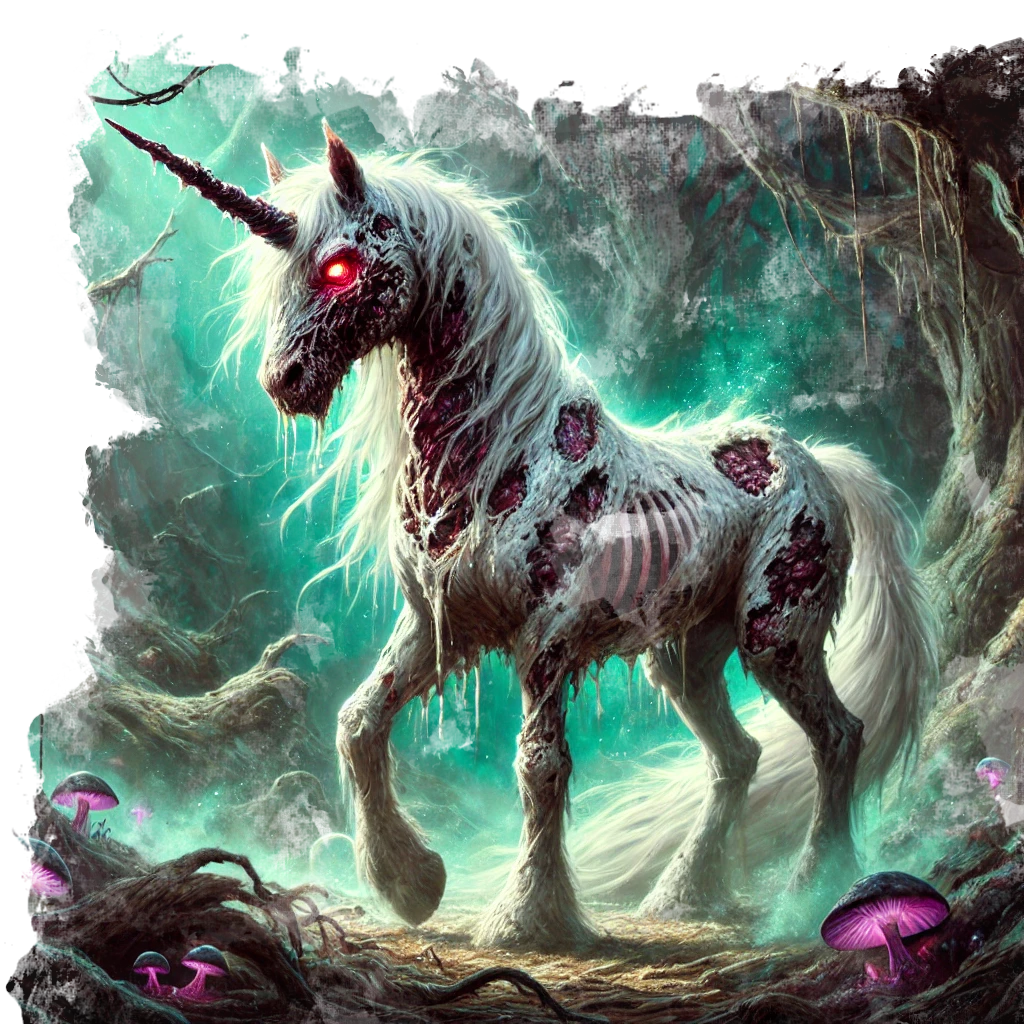
\includegraphics[width=0.55\paperwidth]{monsters/Corrupted_Unicorn}%
      	\end{minipage}%
	};%
\end{tikzpicture}%
\vfill\eject
\begin{DndMonster}[width=0.5\textwidth]{Undead Soldier}
	\DndMonsterType{Medium Undead, chaotic evil}
	
	% If you want to use commas in the key values, enclose the values in braces.
	\DndMonsterBasics[
		armor-class = {16 (Shield)},
		hit-points  = {\DndDice{5d8 + 5}},
		speed       = {30 ft.},
	]
	
	\renewcommand{\AbilityScoreSpacer}{~}
	\DndMonsterAbilityScores[
		str = 14,
		dex = 14,
		con = 12,
		int = 10,
		wis = 11,
		cha = 10,
	]
	
	\DndMonsterDetails[
		saving-throws = {CON +3, WIS +2},
		skills = {Athletics +4},
		%damage-vulnerabilities = {cold},
		damage-resistances = {necrotic},
		damage-immunities = {poison},
		senses = {Darkvision 60 ft., Passive Perception 10},
		condition-immunities = {Poisoned},
		languages = {Common},
		challenge = 1,
	]
	
	\DndMonsterSection{Traits}
    \DndMonsterAction{Martial Advantage}
	Once per turn, the soldier can deal an extra \DndDice{2d6} damage to a creature it hits with a weapon attack if that creature is within 5 feet of an ally of the soldier that isn't incapacitated.
	
	\DndMonsterAction{Undead Fortitude}
	If damage reduces the undead soldier to 0 hit points, it must make a Constitution saving throw with a DC of 5 + the damage taken, unless the damage is radiant or from a critical hit. On a success, the zombie drops to 1 hit point instead.
	
	\DndMonsterAction{Undead Nature}
	The undead doesn't require food, air, drink, or sleep.
	
	\DndMonsterSection{Actions}	
	\DndMonsterAttack[
		name=Longsword,
		distance=melee, % valid options are in the set {both,melee,ranged},
		%type=weapon, %valid options are in the set {weapon,spell}
		mod=+4,
		reach=5,
		%range=20/60,
		targets=one target,
		dmg=\DndDice{1d8 + 2},
		dmg-type=slashing,
		%plus-dmg=\DndDice{1d6},
		%plus-dmg-type=poison,
		or-dmg=\DndDice{1d10 + 2},
		or-dmg-when={ if used with two hands},
		%extra={},
	]
	
	\DndMonsterAttack[
		name=Longbow,
		distance=melee, % valid options are in the set {both,melee,ranged},
		%type=weapon, %valid options are in the set {weapon,spell}
		mod=+4,
		%reach=5,
		range=150/600,
		targets=one target,
		dmg=\DndDice{1d8 + 2},
		dmg-type=piercing,
		%plus-dmg=\DndDice{1d6},
		%plus-dmg-type=poison,
		%or-dmg=,
		%or-dmg-when=,
		%extra={},
	]
\end{DndMonster}
\vfill\eject
\begin{DndMonster}[width=0.5\textwidth]{Wight\phantomsection\addcontentsline{toc}{section}{Wight}\label{monster:Wight}}
	\DndMonsterType{Medium Undead, Chaotic Evil}
	
	% If you want to use commas in the key values, enclose the values in braces.
	\DndMonsterBasics[
		armor-class = {14},
		initiative	= +4,
		hit-points  = {\DndDice{11d8 + 33}},
		speed       = {30 ft.},
	]
	
	\renewcommand{\AbilityScoreSpacer}{~}
	\DndMonsterAbilityScores[
		str = 15,
		dex = 14,
		con = 16,
		int = 10,
		wis = 13,
		cha = 15,
	]
	
	\DndMonsterDetails[
%		saving-throws			= {CON +3, WIS +2},
		skills					= {Perception +3, Stealth +4},
%		damage-vulnerabilities	= {cold},
		damage-resistances		= {Necrotic},
		damage-immunities		= {Poison},
		condition-immunities	= {Exhaustion, Poisoned},
%		gear					= {Leather Armor, Light Crossbow, Scimitar},
		senses					= {Darkvision 60 ft., Passive Perception 13},
		languages				= {Common, Primordial},
		challenge				= 3,
%		proficiency-bonus		= +2,
	]
	
	\DndMonsterSection{Traits}
    \DndMonsterAction{Sunlight Sensitivity}
	While in sunlight, the wight has Disadvantage on ability checks and attack rolls.
	
	\DndMonsterAction{Undead Nature}
	The wight doesn't require food, air, drink, or sleep.
	
	\DndMonsterSection{Actions}	
	\DndMonsterAction{Multiattack}
	The wight makes two attacks, using Necrotic Sword or Necrotic Bow in any combination. It can replace one attack with a use of Life Drain.
	
	\DndMonsterAttack[
		name			= Necrotic Sword,
		distance		= melee,	% valid options are in the set {both,melee,ranged}
%		type			= weapon,	% valid options are in the set {weapon,spell}
		mod				= +4,
		reach			= 5,
%		range			= 20/60,
		targets			= one target,
		dmg				= \DndDice{1d8 + 2},
		dmg-type		= Slashing,
		plus-dmg		= \DndDice{1d8},
		plus-dmg-type	= Necrotic,
%		or-dmg			= \DndDice{1d10 + 2},
%		or-dmg-when		= {},
%		extra			= {},
	]
	
	\DndMonsterAttack[
		name			= Necrotic Bow,
		distance		= ranged,	% valid options are in the set {both,melee,ranged}
%		type			= weapon,	% valid options are in the set {weapon,spell}
		mod				= +4,
%		reach			= 5,
		range			= 150/600,
		targets			= one target,
		dmg				= \DndDice{1d8 + 2},
		dmg-type		= Piercing,
		plus-dmg		= \DndDice{1d8},
		plus-dmg-type	= Necrotic,
%		or-dmg			= \DndDice{1d20},
%		or-dmg-when		= {},
%		extra			= {},
	]
	
	\DndMonsterSpell[
		name		= Life Drain,
		save_skill	= Constitution,
		save_dc		= 13,
		targets		= {one creature within 5 feet},
		failure		= {\DndDice{1d8 + 2} Necrotic damage, and the target's Hit Point maximum decreases by an amount equal to the damage taken.},
%		success		= {},
		extra		= {A Humanoid slain by this attack rises 24 hours later as a Zombie under the wight's control, unless the Humanoid is restored to life or its body is destroyed. The wight can have no more than twelve zombies under its control at a time},
	]
\end{DndMonster}
\vfill\eject
\begin{DndMonster}[width=0.5\textwidth]{Bone Naga\phantomsection\addcontentsline{toc}{section}{Bone Naga}\label{monster:BoneNaga}}
	\DndMonsterType{Large Undead, Neutral Evil}
	
	% If you want to use commas in the key values, enclose the values in braces.
	\DndMonsterBasics[
		armor-class = {15},
		initiative	= +3,
		hit-points  = {\DndDice{10d10 + 10}},
		speed       = {40 ft.},
	]
	
	\renewcommand{\AbilityScoreSpacer}{~}
	\DndMonsterAbilityScores[
		str = 15,
		dex = 16,
		con = 12,
		int = 16,
		wis = 15,
		cha = 15,
	]
	
	\DndMonsterDetails[
%		saving-throws			= {CON +3, WIS +2},
%		skills					= {Athletics +4},
%		damage-vulnerabilities	= {cold},
%		damage-resistances		= {Necrotic},
		damage-immunities		= {Poison},
		condition-immunities	= {Charmed, Exhaustion, Paralyzed, Poisoned},
%		gear					= {Leather Armor, Light Crossbow, Scimitar},
		senses					= {Darkvision 60 ft., Passive Perception 12},
		languages				= {Common, Primordial},
		challenge				= 4,
%		proficiency-bonus		= +2,
	]
	
	\DndMonsterSection{Actions}
    \DndMonsterAction{Martial Advantage}
    The naga makes two Bite attacks. It can replace any attack with a use of Serpentine Gaze.
    
	\DndMonsterAttack[
		name			= Bite,
		distance		= melee,	% valid options are in the set {both,melee,ranged}
%		type			= weapon,	% valid options are in the set {weapon,spell}
		mod				= +5,
		reach			= 10,
%		range			= 20/60,
		targets			= one target,
		dmg				= \DndDice{2d6 + 3},
		dmg-type		= Piercing,
		plus-dmg		= \DndDice{2d6},
		plus-dmg-type	= Necrotic,
%		or-dmg			= \DndDice{1d10 + 2},
%		or-dmg-when		= {},
%		extra			= {},
	]
	
	\DndMonsterSpell[
		name		= Serpentine Gaze,
		save_skill	= Wisdom,
		save_dc		= 13,
		targets		= {one creature the naga can see within 60 feet},
		failure		= {\DndDice{3d6 + 3} Psychic damage, and the target has the Charmed condition until the start of the naga's next turn.},
%		success		= {},
	]
	
	\DndMonsterSection{Spells}
	\begin{DndMonsterSpells}
		\item[Innate Spellcasting] The naga casts one of the following spells, requiring no Material components and using Intelligence as the spellcasting ability (Spell Save DC 13):
		\DndInnateSpellLevel{Mage Hand, Thaumaturgy}
		\DndInnateSpellLevel[1]{Command, Detect Thoughts, Lightning Bolt}
	\end{DndMonsterSpells}
	
\end{DndMonster}

\part*{Test Part}
	
	%https://www.reddit.com/r/Gloryhammer/comments/17srxqi/gloryhammer_dnd_guide_setting_version_1/
	
	
%	\renewcommand\labelitemi{\textbf{\textbullet}}
\end{document}
